% !TEX TS-Program = pdflatex

\documentclass[12pt]{article}
\newcommand{\course}{MA441}
\usepackage{geometry}
\geometry{
    letterpaper,
    left=0.8in,
    top=0.8in,
    headsep=\baselineskip,
    textwidth=26pc,
    marginparsep=2pc,
    marginparwidth=12pc,
    textheight=38\baselineskip,
    headheight=2\baselineskip,
    includemp,
    reversemarginpar,
    bindingoffset=1cm,
    twoside,
    asymmetric
}

\usepackage{amsmath, amsthm}

\usepackage{libertine}  %%%%%The Linux Libertine font family
\usepackage[libertine]{newtxmath}

\usepackage{datetime}
\newdateformat{mydate}{\monthname[\THEMONTH], \THEYEAR}
\newdateformat{lastupdated}{\monthname[\THEMONTH] \THEDAY, \THEYEAR}

\newdateformat{semester}{
  \ifthenelse{\THEMONTH=1}{Winter \THEYEAR}{
    \ifthenelse{\THEMONTH<6}{Spring \THEYEAR}{
      \ifthenelse{\THEMONTH>8}{Fall \THEYEAR}{
        Summer \THEYEAR
      }
    }
  }
}

\usepackage{titling}

\renewcommand{\sectionmark}[1]{ \markright{#1}{} }

\usepackage{fancyhdr}
\pagestyle{fancy}

\fancyhf{}
\fancyhfoffset[L]{14pc}

\renewcommand{\headrulewidth}{1pt}
\renewcommand{\footrulewidth}{1pt}
\fancyhead[RE,LO]{\bf \course}
% \fancyhead[RO,LE]{\thepage}
\fancyhead[C]{\large\bf \leftmark}
\fancyfoot[RE, LO]{\raisebox{-10\baselineskip}{\semester{\thedate}}}
\fancyfoot[RO, LE]{\raisebox{-10\baselineskip}{\hfill \sffamily \theauthor}\hspace{-1ex}}
\fancyfoot[C]{\raisebox{-10\baselineskip}{\thepage}}

\usepackage{ifthen}
\usepackage{xparse}
\usepackage{ifoddpage}

\usepackage{eso-pic}

\NewDocumentCommand{\addBG}{}{
  \AddToShipoutPicture{
    \AtTextLowerLeft{
      \put(-1pc,\LenToUnit{-\baselineskip}){
        \rule[0em]{1.5pt}{\dimexpr \textheight+2\baselineskip}
      }
    }
  }
}

\NewDocumentCommand{\newlecture}{}{
  \newpage
  \checkoddpage
  \ifoddpage
  \else
    \clearpage
    \thispagestyle{empty}
    \ClearShipoutPictureBG
    \cleardoublepage
    \newpage
    \addBG
  \fi
}


\usepackage[
  breaklinks = true,
  colorlinks = true,
  pdftitle = "Calculus I Worksheets",
  pdfauthor = "Dr. Ye"
]{hyperref}
\usepackage{bookmark}
\usepackage{longtable}
\usepackage{calc}
\usepackage{booktabs}
\usepackage{array}
\usepackage{multirow}
\usepackage{multicol}
\usepackage{float}
\usepackage{colortbl}
\usepackage{pdflscape}
\usepackage{tabu}
\usepackage{threeparttable}
\usepackage{threeparttablex}
\usepackage[normalem]{ulem}
\usepackage{makecell}
\usepackage{xcolor}

\usepackage{changepage}
\newenvironment{fullwidth}{%
  \begin{adjustwidth}{-14pc}{}%
  \hsize=\linewidth%
}{\end{adjustwidth}}

\usepackage[inline]{enumitem}
\setenumerate{
	label=\textup{(\arabic*)},
	% afterlabel={\quad},
	%%vertical
	topsep=0pt,
	partopsep=0pt,
	itemsep=5\baselineskip,
	parsep=2pt,
  after=\vspace*{\dimexpr 5\baselineskip},
	% labelindent=0em,
	% itemindent = *,
	itemindent=1ex,
	wide,
	itemjoin={\hspace{\fill}},
	%%Horizontal
}
\setitemize{
	%%vertical
	topsep=0pt,
	partopsep=0pt,
	itemsep=0pt,
	parsep=0pt,
	%%Horizontal
	labelindent=0em,
	leftmargin =!,
	itemindent = 0pt,
	labelsep= 2pt,
	labelwidth=1em,
}
\setlist{topsep=0pt}

\SetEnumitemKey{sepno}{nosep, after=\vspace*{0pt}}

\SetEnumitemKey{twocol}{
itemsep = 1\itemsep,
parsep = 1\parsep,
before = \raggedcolumns\begin{multicols}{2},
after = \end{multicols}}

\usepackage{tikz}
\usepackage{pgfplots}
\pgfplotsset{compat=newest}
\usepackage{pgfmath}
\usepackage{tikz-cd}
\usepackage{pgffor}
\usepackage{tkz-euclide}
\usepgfplotslibrary{fillbetween}
\usetikzlibrary{
	calc,
	angles,
	quotes,
	arrows.meta,
	math,
	backgrounds,
	pgfplots.statistics,
	matrix,
	patterns,
	shapes.geometric,
	spy,
    intersections,
    decorations.markings,
    decorations.pathmorphing,
    decorations.pathreplacing,
    decorations.shapes
}
\pgfdeclarelayer{ft}
\pgfdeclarelayer{bg}
\pgfsetlayers{bg,main,ft}
%%%%%%%%%%%%%%%%%%%%%%%%%%%%%%%%%%%%%%%%%%%%%%%%%%%%%%%%%%%%%%%%%%%%

%%%%%%%%%%%%%%%%% Setup the Coordinate System %%%%%%%%%%%%%%%%%%%%%%
\pgfplotsset{every axis/.style={
			%		 axis equal image,
			axis x line=middle,    % put the x axis in the middle
			axis y line=middle,    % put the y axis in the middle
			axis line style={-latex,very thick}, % arrows on the axis
			xlabel={$x$},          % default put x on x-axis
			ylabel={$y$},          % default put y on y-axis
			xlabel style = {font=\tiny, at={(xticklabel* cs:1)}, anchor=south},
			ylabel style = {font=\tiny, at={(yticklabel* cs:1)}, anchor=west},
			scaled ticks=true,
			x tick label style={font=\tiny, yshift=0.25ex, inner xsep=0pt},
			y tick label style={font=\tiny, xshift=0.25ex, inner ysep=0pt},
			grid style={black},
			% set layers=standard,
		}
}

%%%%%%%%%%%%%%% include files/Figure %%%%%%%%%%%%%%%%%%%%%%%%%%%%%%%%%
\usepackage{import}
% \usepackage{subfiles}
\usepackage[verbose]{wrapfig}
%%%%%%%%%%%%%%%%%%%%%%%%%%%%%%%%%%%%%%%%%%%%%%%%%%%%%%%%%%%%%%%%%

%%%%%%%%%%%%%%%% Cancel common factors in Math %%%%%%%%%%%%%%%%%%%%
\usepackage[makeroom]{cancel}
%%%%%%%%%%%%%%%%%%%%%%%%%%%%%%%%%%%%%%%%%%%%%%%%%%%%%%%%%%%%%%%%%%%

%%%%%%%%%%%%%% Math mode without vertical spacing %%%%%%%%%%%%%%%%%
\makeatletter
\g@addto@macro\normalsize{%
	\setlength\abovedisplayskip{1pt plus 2pt minus 2pt}%
	\setlength\belowdisplayskip{1pt plus 2pt minus 2pt}%
	\setlength\abovedisplayshortskip{1pt plus 2pt minus 2pt}%
	\setlength\belowdisplayshortskip{1pt plus 2pt minus 2pt}%
}
\makeatother
%%%%%%%%%%%%%%%%%%%%%%%%%%%%%%%%%%%%%%%%%%%%%%%%%%%%%%%%%%%%%%%%

\newcommand{\ZZ}{\mathbf{Z}}
\newcommand{\RR}{\mathbf{R}}
\newcommand{\NN}{\mathbf{N}}
\newcommand{\QQ}{\mathbf{Q}}
\newcommand{\abs}[1]{\lvert #1\rvert}
\newcommand{\ii}{\mathbf{i}}
\newcommand{\parll}{ {\mathbin{\parallel}} }
\newcommand{\prll}{{\mathbin{\!/\mkern-5mu/\!}}}

\makeatletter
\renewcommand*\rel@kern[1]{\kern#1\dimexpr\macc@kerna}
\renewcommand*\widebar[1]{%
\begingroup
\def\mathaccent##1##2{%
\rel@kern{0.8}%
\overline{\rel@kern{-0.8}\macc@nucleus\rel@kern{0.2}}%
\rel@kern{-0.2}%
}%
\macc@depth\@ne
\let\math@bgroup\@empty \let\math@egroup\macc@set@skewchar
\mathsurround\z@ \frozen@everymath{\mathgroup\macc@group\relax}%
\macc@set@skewchar\relax
\let\mathaccentV\macc@nested@a
\macc@nested@a\relax111{#1}%
\endgroup
}
\renewcommand{\bar}{\widebar}
\newcommand*\centermath[1]{\omit\hfil~$\displaystyle#1$~\hfil\ignorespaces}
\newcommand{\cmc}{\centermath}
\newcommand*\ctc[1]{\omit\hfil\quad~ #1 ~\quad\hfil\ignorespaces}
\newcommand{\dfn}[1]{\textit{\textbf{#1}}}


\theoremstyle{plain}% default
\newtheorem{theorem}{Theorem}[section]
\newtheorem{lemma}[theorem]{Lemma}
\newtheorem{proposition}[theorem]{Proposition}
\newtheorem{corollary}[theorem]{Corollary}
\theoremstyle{definition}
\newtheorem{definition}[theorem]{Definition}
\newtheorem{example}{Example}[section]
\newtheorem{exercise}{Exercise}[section]
\theoremstyle{remark}
\newtheorem*{remark}{Remark}
\newtheorem*{note}{Note}
\newtheorem{case}{Case}


\title{\course~Worksheets}
\author{Dr. Ye}
\date{\semester{\today}}


\begin{document}
\newgeometry{margin=1in}
\clearpage
\ClearShipoutPictureBG

\begin{titlepage}
  \vspace{2\baselineskip}
  \maketitle
  \thispagestyle{empty}
  \vfill
  \centering{
  \small
  Last updated on \lastupdated{\today}\\
  
  License: \href{CC BY-NC-SA}{https://creativecommons.org/licenses/by-nc-sa/4.0/}
  } 
  \vspace{3\baselineskip}
\end{titlepage}

\newpage
\addBG

\restoregeometry

\newlecture
% !TeX root = main.tex

\hypertarget{limits-of-functions}{%
\section{Limits of Functions}\label{limits-of-functions}}

\hypertarget{intuitive-definition}{%
\subsection{Intuitive definition}\label{intuitive-definition}}

\noindent\textbf{Limits:}

We say that the limit of \(f(x)\) as \(x\) approaches \(a\) is \(L\) if $f(x)$ can get arbitrarily close to $L$ when \(x\) approaches to \(a\). 

\[\lim\limits_{x \to a} f(x)=L\]

\noindent\textbf{Limit from the left:}

We say that \(L\) is the left limit of \(f(x)\) if $f(x)$ can get arbitrarily close to $L$ when \(x\) approaches to \(a\) from the left.

\[\lim\limits_{x \to a^{-} }f(x)=L.\]

\textbf{Limit from the right:}

We say that \(L\) is the right limit of \(f(x)\) if $f(x)$ can get arbitrarily close to $L$ when \(x\) approaches to \(a\) from the right.

\[\lim\limits_{x \to a^+}f(x)=L.\]

\hypertarget{determine-limits-from-graphs}{%
\subsection{Determine limits from
graphs}\label{determine-limits-from-graphs}}

\begin{example}
  Using the graph of the function \(f\) shown below to
  determine the limit \(\lim\limits_{x\to -4}f(x)\) and the limit
  \(\lim\limits_{x\to 2} f(x)\).
  
  \begin{figure}[h]
    \centering
  \href{https://www.geogebra.org/m/Ktr9uqYu}{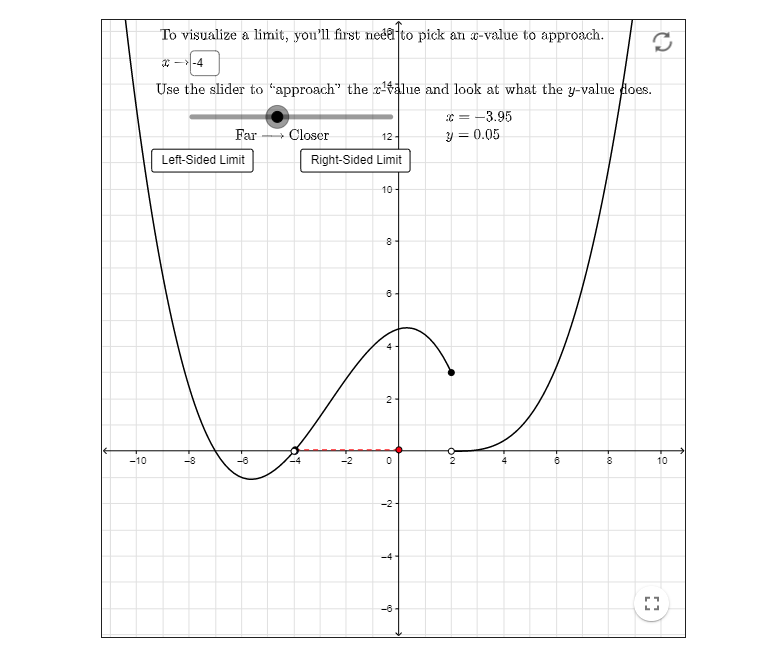
\includegraphics[height=0.3\textheight]{img/clip_image001.png}}
  \end{figure}
\end{example}
\vspace*{2\baselineskip}

\begin{example}
  Using the graph of the function \(g\) to evaluate the
  limit \(\lim\limits_{x\to -1}g(x)\).
  
  \begin{figure}[h]
  \centering
  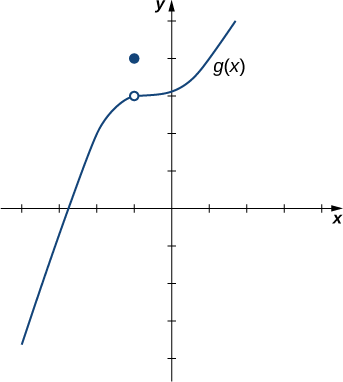
\includegraphics[scale=0.8]{img/imageedit_9_2225331012.png}
  \end{figure}
\end{example}
\vspace*{2\baselineskip}

\hypertarget{determine-limits-numerically-using-tables}{%
\subsection{Determine limits numerically using
tables}\label{determine-limits-numerically-using-tables}}

Numerically, we say that
\(\lim\limits_{x\to a}f(x)=L\) if for any \(\varepsilon>0\) there exists
a number \(\delta>0\) such that \(|f(x)-L|<\varepsilon\) whenever
\(|x-a|<\delta\).

\begin{example}
  Use a table to determine the limit
  \(\lim\limits_{x\to 1}x\).
\end{example}
\vspace*{6\baselineskip}

\begin{example}
  Use a table to determine the limit
  \(\lim\limits_{x\to 1}c\), where \(c\) is a constant number.
\end{example}
\vspace*{6\baselineskip}

\begin{example}
  Use a table to determine the limit
  \(\lim\limits_{x\to 0}\dfrac{\sin x}{x}\).
\end{example}
\vspace*{6\baselineskip}

\begin{example}
  Use a table to determine the limit
  \(\lim\limits_{x\to 0}\sin\left(\frac1x\right)\).
\end{example}
\vspace*{6\baselineskip}

\subsection{One-sided limits}

\begin{example}
  For the function
  \(f(x)=\begin{cases}x+1, & \text{if }x<2\\ x^2-4, & \text{if }x\ge 2\end{cases}\),
  determine each of the following limits.
  
  \begin{enumerate}
  \item
    \(\lim\limits_{x \to 2^-}f(x)\)
  \item
    \(\lim\limits_{x \to 2^+}f(x)\)
  \item
    \(\lim\limits_{x\to 2}f(x)\)
  \end{enumerate}
\end{example}

\begin{example}
  For the function
  \(f(x)=\begin{cases}x^2+1, & \text{if }x<1\\ 3x-1, & \text{if }x\ge 1\end{cases}\),
  determine each of the following limits.
  
  \begin{enumerate}
  \item
    \(\lim\limits_{x \to 1^-}f(x)\)
  \item
    \(\lim\limits_{x \to 1^+}f(x)\)
  \item
    \(\lim\limits_{x\to 1}f(x)\)
  \end{enumerate}
\end{example}

\begin{theorem}
  Let \(f(x)\) be a function defined at all values in an
  open interval containing \(a\), with the possible exception of \(a\)
  itself, and let \(L\) be a real number. Then,
  \[\lim\limits_{x \to a}f(x)=L\]
  if and only if \(\lim\limits_{x \to a^-}f(x)=L\) and
  \(\lim\limits_{x \to a^+} f(x)=L\).
\end{theorem}

\hypertarget{infinite-limits}{%
\subsection{Infinite limits}\label{infinite-limits}}

\textbf{Infinite limits from the left:} Let \(f(x)\) be a function
defined at all values in an open interval of the form \((b,a)\).

\begin{enumerate}[sepno]
\item
  If the values of \(f(x)\) can be arbitrarily large as the values of
  \(x\) (where \(x<a\)) approach the number \(a\), then we say that the
  limit as \(x\) approaches \(a\) from the left is positive infinity and
  we write \[\lim\limits_{x \to a^-}f(x)=+\infty.\]
\item
  If the values of \(f(x)\) can be arbitrarily large as the values of
  \(x\) (where \(x<a\)) approach the number \(a\), then we say that the
  limit as \(x\) approaches \(a\) from the left is negative infinity and
  we write \[\lim\limits_{x \to a^-}f(x)=-\infty.\]
\end{enumerate}

\textbf{Infinite limits from the right:} Let \(f(x)\) be a function
defined at all values in an open interval of the form \((a,c)\).

\begin{enumerate}[sepno]
\item
  If the values of \(f(x)\) can be arbitrarily large as the values of
  \(x\) (where \(x>a\)) approach the number \(a\), then we say that the
  limit as \(x\) approaches \(a\) from the left is positive infinity and
  we write \[\lim\limits_{x \to a^+}f(x)=+\infty.\]
\item
  If the values of \(-f(x)\) can be arbitrarily large as the values of
  \(x\) (where \(x>a\)) approach the number \(a\), then we say that the
  limit as \(x\) approaches \(a\) from the left is negative infinity and
  we write \[\lim\limits_{x \to a^+}f(x)=-\infty.\]
\end{enumerate}

\textbf{Two-sided infinite limit:} Let \(f(x)\) be defined for all
\(x\neq a\) in an open interval containing \(a\)

\begin{enumerate}[parsep=0pt,after=\vspace{0pt}]
\item
  If the values of \(f(x)\) can be arbitrarily large as the values of
  \(x\) (where \(x\neq a\)) approach the number \(a\), then we say that the
  limit as \(x\) approaches \(a\) is positive infinity and we write
  \[\lim\limits_{x \to a} f(x)=+\infty.\]
\item
  If the values of \(-f(x)\) can be arbitrarily large as the values of
  \(x\) (where \(x\neq a\)) approach the number \(a\), then we say that the
  limit as \(x\) approaches \(a\) is negative infinity and we write
  \[\lim\limits_{x \to a}f(x)=-\infty.\]
\end{enumerate}

\begin{example}
  Evaluate each of the following limits, if possible.
  
  \begin{enumerate}
  \item
    \(\lim\limits_{x \to 0^-} \frac{1}{x}\)
  \item
    \(\lim\limits_{x \to 0^+} \frac{1}{x}\)
  \item
    \(\lim\limits_{x \to 0}\frac{1}{x}\)
  \end{enumerate}
\end{example}

\subsection{Practice}


\begin{exercise}
  Use the graph of \(h(x)\) shown below to determine
  the limit \(\lim\limits_{x \to 2}h(x)\).
  
  \begin{figure}[h!]
  \centering
  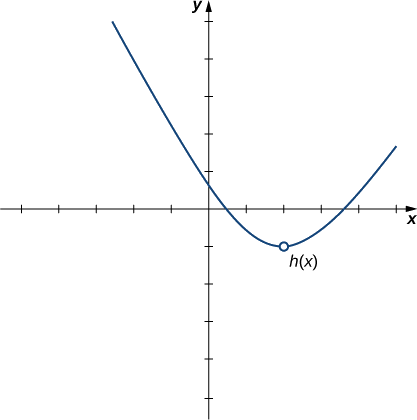
\includegraphics[scale=0.8]{img/imageedit_13_2727890618.png}
  \end{figure}
\end{exercise}
\vspace*{\baselineskip}


\begin{exercise}
  Determine the limit
  \(\lim\limits_{x\to 1}\dfrac{\frac1x-1}{x-1}\).
\end{exercise}
\vspace*{6\baselineskip}

\begin{exercise}
  Determine the limit
  \(\lim\limits_{x\to 0}x\sin\left(\frac1x\right)\).
\end{exercise}
\vspace*{6\baselineskip}

\begin{exercise}
  Determine the limits
  
  \begin{enumerate}
  \item
    \(\lim\limits_{x\to 1^-}\dfrac{|x-1|}{x-1}\).
  \item
    \(\lim\limits_{x\to 1^+}\dfrac{|x-1|}{x-1}\).
  \item
    \(\lim\limits_{x\to 1^+}\dfrac{|x-1|}{x-1}\).
  \end{enumerate}
\end{exercise}

\begin{exercise}
  Evaluate each of the following limits, if possible.
  
  \begin{enumerate}
  \item
    \(\lim\limits_{x \to 0^-}\frac{1}{x^2}\)
  \item
    \(\lim\limits_{x \to 0^+}\frac{1}{x^2}\)
  \item
    \(\lim\limits_{x \to 0}\frac{1}{x^2}\)
  \end{enumerate}
\end{exercise}


\newlecture
% !TeX root = main.tex

\section{Limit Laws}

\hypertarget{limits-under-arithmetical-operations}{%
\subsection{Limits under arithmetical
operations}\label{limits-under-arithmetical-operations}}

\noindent\textbf{Basic Limit Results}

For any real number \(a\) and any constant \(c\),

\begin{enumerate}[sepno]
\item
  \(\lim\limits_{x\to a}x=a\)
\item
  \(\lim\limits_{x\to a}c=c\)
\end{enumerate}

Let \(f(x)\) and \(g(x)\) be defined for all \(x\neq a\) over some open
interval containing \(a\). Assume that \(L\) and \(M\) are real numbers
such that \(\lim\limits_{x\to a}f(x)=L\) and
\(\lim\limits_{x\to a}g(x)=M\). Let \(c\) be a constant. Then, each of
the following statements holds:

\begin{itemize}[parsep=0pt, after=\vspace{0pt}]
\item
  \textbf{Sum law for limits}:

\[\lim\limits_{x\to a}(f(x)+g(x))=\lim\limits_{x\to a}f(x)+\lim\limits_{x\to a}g(x)=L+M\]

\item
  \textbf{Difference law for limits}:

\[\lim\limits_{x\to a}(f(x)-g(x))=\lim\limits_{x\to a}f(x)-\lim\limits_{x\to a}g(x)=L-M\]

\item
  \textbf{Constant multiple law for limits}:

\[\lim\limits_{x\to a}cf(x)=c\cdot \lim\limits_{x\to a}f(x)=cL\]

\item
  \textbf{Product law for limits}:

\[\lim\limits_{x\to a}(f(x)\cdot g(x))=\lim\limits_{x\to a}f(x)\cdot \lim\limits_{x\to a}g(x)=L\cdot M\]

\item
  \textbf{Quotient law for limits}:

\[\lim\limits_{x\to a}\frac{f(x)}{g(x)}=\frac{\lim\limits_{x\to a}f(x)}{\lim\limits_{x\to a}g(x)}=\frac{L}{M}\]

for \(M\neq 0\).

\item
  \textbf{Power law for limits}:

\[\lim\limits_{x\to a}\big(f(x)\big)^n=\big(\lim\limits_{x\to a}f(x)\big)^n=L^n\]

for every positive integer \(n\).

\item
  \textbf{Root law for limits}:
  
  \[\lim\limits_{x\to a}\sqrt[n]{f(x)}=\sqrt[n]{\lim\limits_{x\to a} f(x)}=\sqrt[n]{L}\]
  
  for all \(L\) if \(n\) is odd and for \(L\geq 0\) if \(n\) is even.
  
\end{itemize}



\begin{theorem}
  Let \(p(x)\) and \(q(x)\) be polynomial functions. Let \(a\) be a real
  number. Then,
  
  \[\lim\limits_{x\to a}\frac{p(x)}{q(x)}=\frac{p(a)}{q(a)}\] when
  \(q(a)\neq 0\).
\end{theorem}


\begin{example}
Evaluate
\(\lim\limits_{x\to 2}\frac{2x^2-3x+1}{x^3+4}\)
\end{example}
\vspace*{6\baselineskip}

\begin{example}
Evaluate
\(\lim\limits_{x\to 1}\sqrt{\frac{5x^2-1}{x^3+1}}\)
\end{example}
\vspace*{6\baselineskip}

The following observation allows us to evaluate many limits of the type
that the function \(f\) is undefined at \(a\) but a function \(g\)
equivalent to \(f\) away from \(a\) is well defined at \(a\).

\begin{theorem}
  If for all \(x\neq a,\;f(x)=g(x)\) over some open interval
  containing \(a\), then
  
  \[\lim\limits_{x\to a}f(x)=\lim\limits_{x\to a}g(x).\]
\end{theorem}

\begin{example}
Evaluate
\(\lim\limits_{x\to-3}\dfrac{\dfrac{1}{x+2}+1}{x+3}\).
\end{example}
\vspace*{6\baselineskip}

\begin{example}
Evaluate
\(\lim\limits_{x\to-1}\dfrac{\sqrt{x+2}-1}{x+1}\).
\end{example}
\vspace*{6\baselineskip}

\begin{example}
Evaluate
\(\lim\limits_{x\to3}\left(\dfrac{1}{x-3}-\dfrac{4}{x^2-2x-3}\right)\).
\end{example}
\vspace*{6\baselineskip}

\begin{theorem}[Squeeze Theorem]
  Let \(f(x),g(x)\), and \(h(x)\) be defined for all \(x\neq a\) over an open
  interval containing \(a\). If
  
  \[f(x)\le g(x)\le h(x)\]
  
  for all \(x\neq a\) in an open interval containing \(a\) and
  
  \[\lim\limits_{x\to a}f(x)=L=\lim\limits_{x\to a}h(x)\]
  
  where \(L\) is a real number, then \(\lim\limits_{x\to a}g(x)=L.\)
\end{theorem}
\marginpar{
  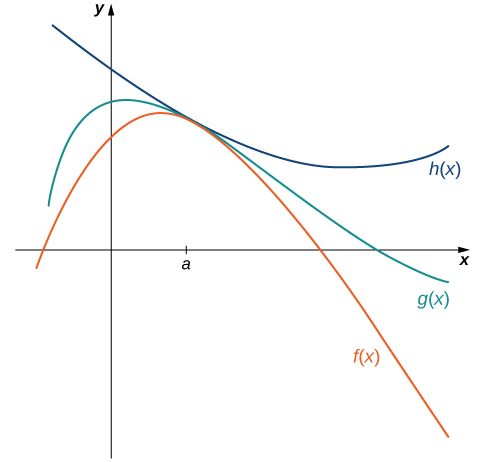
\includegraphics[scale=0.5]{img/CNX_Calc_Figure_02_03_005.jpeg}
}


\begin{example}
  Evaluate the limit
  \(\lim\limits_{x\to 0}\dfrac{\sin x}{x}\)
  
\begin{fullwidth}
  \begin{figure}[h!]
  \centering
  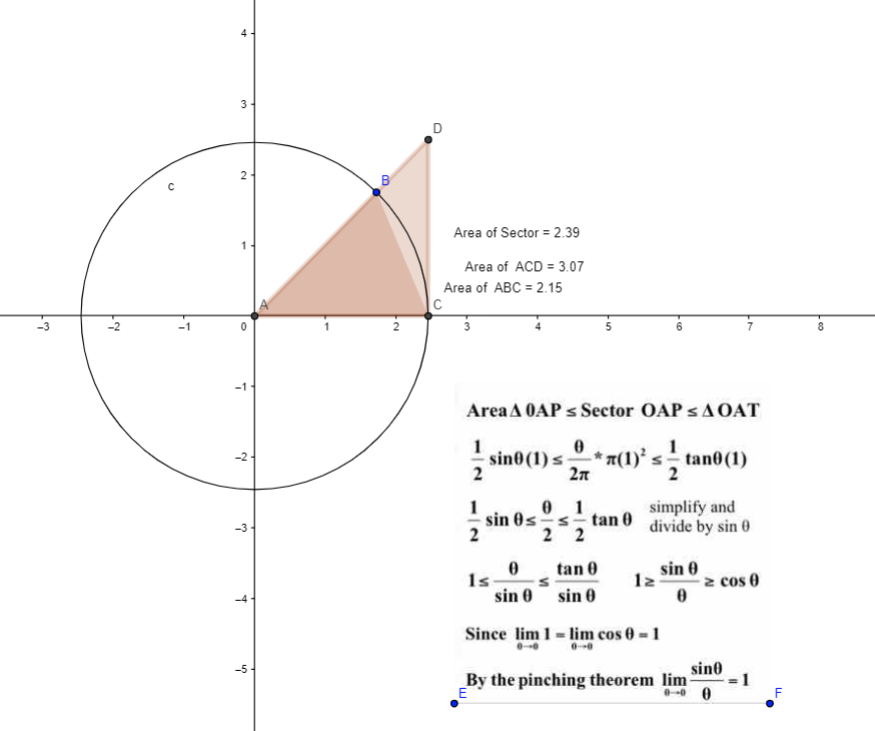
\includegraphics[width=0.8\linewidth]{img/image-20200830170927969.png}
  \end{figure}
\end{fullwidth}
\end{example}
\vspace*{6\baselineskip}

  
\begin{example}
Use the squeeze theorem to evaluate
\(\lim\limits_{x\to0}x^2\sin\dfrac{1}{x}\).

\href{https://www.geogebra.org/m/gb9uqf9u}{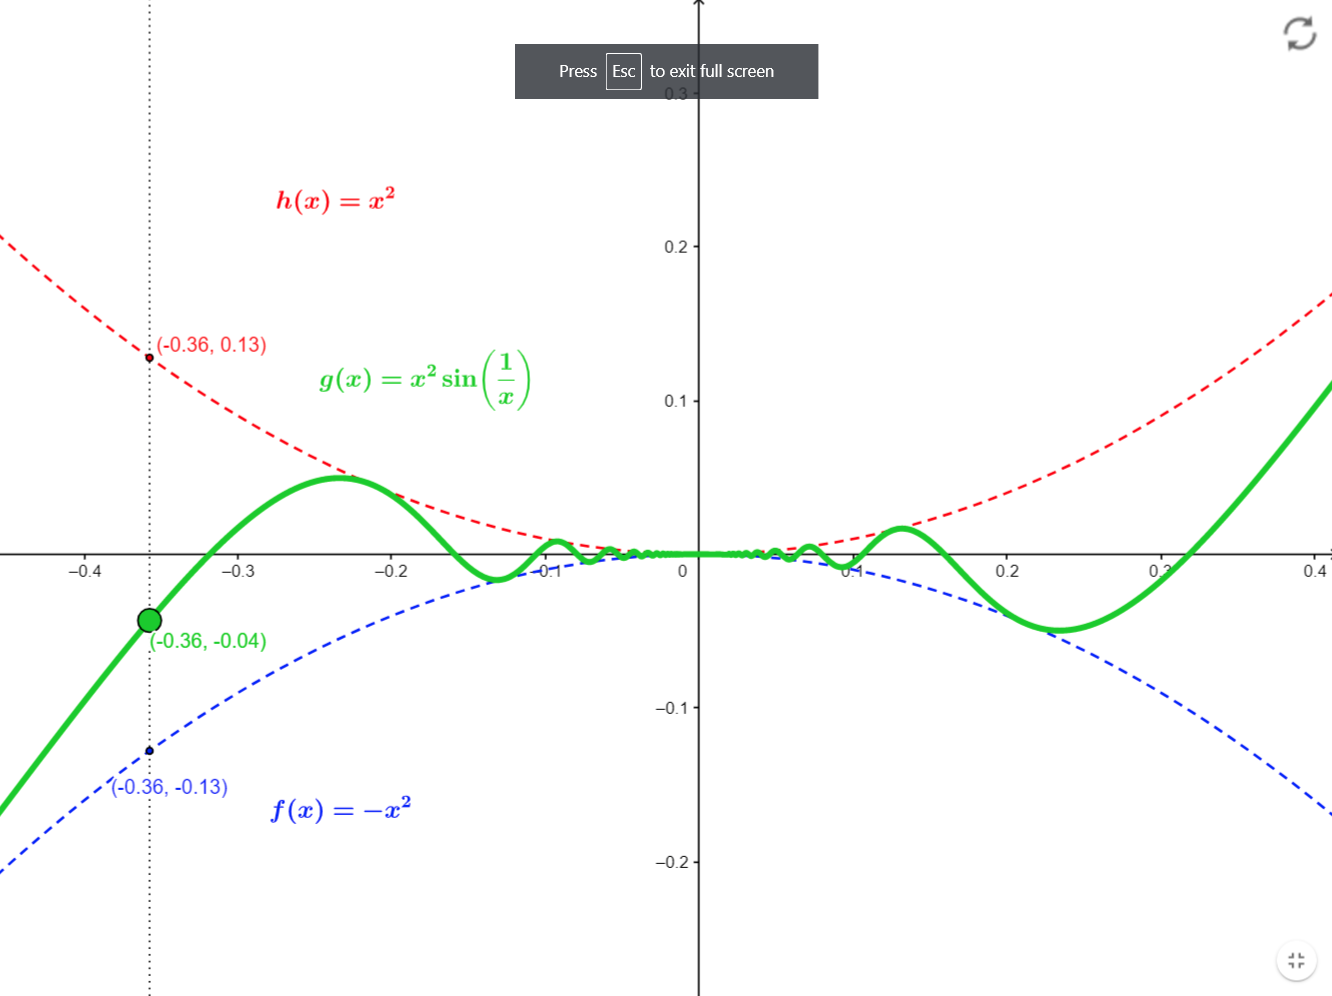
\includegraphics[width=0.9\textwidth]{img/image-20200830161044604.png}}
\end{example}
\vspace*{6\baselineskip}

\begin{example}
Suppose that
\(\lim\limits_{x\to a}\lvert f(x)-2\rvert =0\). Evaluate the limit
\(\lim\limits_{x\to a}f(x)\).
\end{example}
\vspace*{6\baselineskip}

\hypertarget{limits-of-indeterminate-forms}{%
\subsection{Limits of indeterminate
forms}\label{limits-of-indeterminate-forms}}

Some limits of indeterminate forms, such as \(\frac00\),
\(\frac{\infty}{\infty}\), \(0\cdot \infty\), and \(\infty-\infty\), can
be evaluated using algebraic methods. Here are some examples.

\begin{example}
Evaluate the limit
\(\lim\limits_{x\to 0}\dfrac{1-\cos x}{x}\)
\end{example}
\vspace*{6\baselineskip}

\begin{proposition}
  Let \(f\) be function defined near \(0\) and \(b\)
  be number. If \(\lim\limits_{x\to 0}\dfrac{f(x)}{x}=L\) and
  \(b \neq 0,\) then \(\lim\limits_{x \to 0}\dfrac{f(bx)}{x}=bL\).
\end{proposition}

\begin{example}
Evaluate the limit
\(\lim\limits_{\theta\to 0}\frac{\sin(3\theta)}{5\theta}\)
\end{example}
\vspace*{6\baselineskip}

\begin{example}
Evaluate
\(\lim\limits_{x\to 2}\left(\dfrac1{x^2-2x}-\dfrac{1}{2x-4}\right)\).
\end{example}
\vspace*{6\baselineskip}

\subsection{Apply limit laws to infinite
limits}

Limit laws mostly work for infinite limits. However, one should be very
careful when apply a limit laws with infinite limits.

\begin{example}
Evaluate \(\lim\limits_{x\to2^-}\dfrac{x-3}{x^2-2x}\).
\end{example}
\vspace*{6\baselineskip}

\subsection{Practice}

\begin{exercise}
  Evaluate
  \(\lim\limits_{x\to -1}\sqrt{\frac{8x^2-9x+10}{x^2+2}}\)
  \end{exercise}
  \vspace*{6\baselineskip}

\begin{exercise}
Evaluate \(\lim\limits_{x\to 3}\dfrac{x^2-9}{x-3}\).
\end{exercise}
\vspace*{6\baselineskip}

\begin{exercise}
Evaluate
\(\lim\limits_{x\to 49}\dfrac{\sqrt{x}-7}{x-49}\).
\end{exercise}
\vspace*{6\baselineskip}

\begin{exercise}
Evaluate
\(\lim\limits_{x\to 0}\lvert x\rvert \sin\left(\frac{1}{x}\right)\)
\end{exercise}
\vspace*{6\baselineskip}

\begin{exercise}
Evaluate
\(\lim\limits_{x\to 1}\left(\dfrac1{x^2-x}-\dfrac{1}{2x^2-3x+1}\right)\).
\end{exercise}
\vspace*{6\baselineskip}

\begin{exercise}
Evaluate the limit
\(\lim\limits_{t\to 0}\dfrac{\cos(3t)-1}{\sin t}\)
\end{exercise}
\vspace*{6\baselineskip}

\begin{exercise}
Evaluate
\(\lim\limits_{x\to 1}\dfrac{x+2}{(x-1)^2}\).
\end{exercise}
\vspace*{6\baselineskip}


\newlecture
% !TeX root = main.tex

\hypertarget{continuity}{%
\section{Continuity}\label{continuity}}

\hypertarget{continuous-at-a-point}{%
\subsection{Continuous at a point}\label{continuous-at-a-point}}

\begin{definition}

A function \(f(x)\) is continuous at a point \(a\) if and only if the
following three conditions are satisfied:

\begin{enumerate}[sepno]
\item
  \(f(a)\) is defined
\item
  \(\lim\limits_{x\to a}f(x)\) exists
\item
  \(\lim\limits_{x\to a}f(x)=f(a)\)
\end{enumerate}

A function is discontinuous at a point \(a\) if it fails to be
continuous at \(a\).

\end{definition}

\begin{example}
Using the definition,
determine whether the function \(f(x)=\dfrac{x^2-4}{x-2}\) is continuous
at \(x=2\). Justify the conclusion.

\end{example}
\vspace*{6\baselineskip}

\begin{example}

Determining Continuity at a Point, Condition 2 Using the definition,
determine whether the function
\(f(x)=\begin{cases}-x^2+4, & \mathrm{if} \; x\le 3 \\ 4x-8, & \mathrm{if} \; x>3\end{cases}\)
is continuous at \(x=3\). Justify the conclusion.

\end{example}
\vspace*{6\baselineskip}

\begin{example}

Determining Continuity at a Point, Condition 3**\\
Using the definition, determine whether the function
\(f(x)=\begin{cases}\frac{\sin x}{x}, & \text{if } x\ne 0\\1, & \text{if } x=0\end{cases}\)
is continuous at \(x=0\).

\end{example}
\vspace*{6\baselineskip}

\hypertarget{discontinuities}{%
\subsection{Discontinuities}\label{discontinuities}}

\begin{definition}

If \(f(x)\) is discontinuous at \(a\), then

\begin{enumerate}[sepno]
\item
  \(f\) has a removable discontinuity at \(a\) if
  \(\lim\limits_{x\to a}f(x)\) exists. (Note: When we state that
  \(\lim\limits_{x\to a}f(x)\) exists, we mean that
  \(\lim\limits_{x\to a}f(x)=L\), where L is a real number.)
\item
  \(f\) has a jump discontinuity at \(a\) if
  \(\lim\limits_{x\to a^-}f(x)\) and \(\lim\limits_{x\to a^+}f(x)\) both
  exist, but
  \(\lim\limits_{x\to a^-}f(x)\neq \lim\limits_{x\to a^+}f(x)\). (Note:
  When we state that \(\lim\limits_{x\to a^-}f(x)\) and
  \(\lim\limits_{x\to a^+}f(x)\) both exist, we mean that both are
  real-valued and that neither take on the values \(\pm\infty\).)
\item
  \(f\) has an infinite discontinuity at \(a\) if
  \(\lim\limits_{x\to a^-}f(x)=\pm\infty\) or
  \(\lim\limits_{x\to a^+}f(x)=\pm\infty\).
\end{enumerate}

\end{definition}

\begin{fullwidth}
  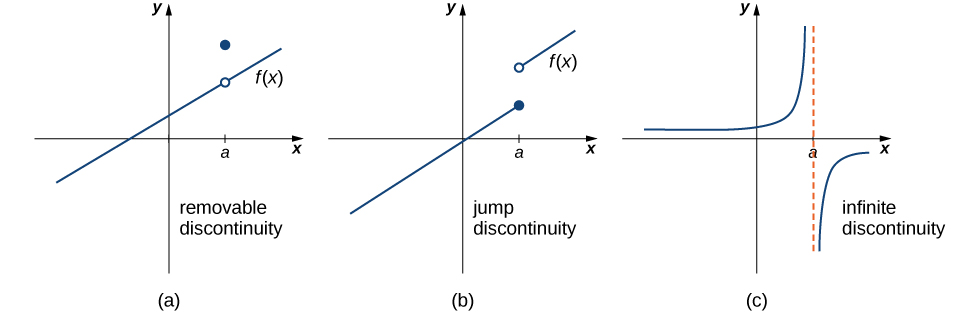
\includegraphics[width=1.2\textwidth]{img/2020-09-02-22-17-09.png}
\end{fullwidth}

\begin{example}

In Example, we showed that \(f(x)=\dfrac{x^2-4}{x-2}\) is discontinuous
at \(x=2\). Classify this discontinuity as removable, jump, or infinite.

\end{example}
\vspace*{6\baselineskip}

\hypertarget{continuity-from-the-right-and-from-the-left}{%
\subsection{Continuity from the right and from the
left}\label{continuity-from-the-right-and-from-the-left}}

\begin{definition}

  A function \(f(x)\) is said to be continuous from the right at a if
  \(\lim\limits_{x\to a^+}f(x)=f(a)\).
  
  A function \(f(x)\) is said to be continuous from the left at a if
  \(\lim\limits_{x\to a^-}f(x)=f(a)\)

\end{definition}

\hypertarget{continuity-over-an-interval}{%
\subsection{Continuity over an
interval}\label{continuity-over-an-interval}}

\begin{definition}

A function is continuous over an open interval if it is continuous at
every point in the interval. A function \(f(x)\) is continuous over a
closed interval of the form \([a,b]\) if it is continuous at every point
in \((a,b)\) and is continuous from the right at a and is continuous
from the left at b. Analogously, a function \(f(x)\) is continuous over
an interval of the form \((a,b]\) if it is continuous over \((a,b)\) and
is continuous from the left at b. Continuity over other types of
intervals are defined in a similar fashion.

\end{definition}

\begin{theorem}[Rules of continuity]

  Let \(f\) and \(g\) be two
functions continuous over an interval \(I\). Then

\begin{enumerate}[sepno]
\item
  the linear combination \(af+bg\) is continuous over the interval
  \(I\);
\item
  the multiplication \(f\cdot g\) is continuous over the interval \(I\);
\item
  the quotient \(\dfrac{f}{g}\) is continuous over the intersection of
  \(I\) and domain of \(g\).
\end{enumerate}
\end{theorem}

\begin{corollary}

Polynomials and rational functions are continuous over their domains.

\end{corollary}


\begin{example}

State the interval(s) over which the function
\(f(x)=\dfrac{x-1}{x^2+2x}\) is continuous.

\end{example}
\vspace*{6\baselineskip}

\begin{example}

State the interval(s) over which the function \(f(x)=\sqrt{4-x^2}\) is
continuous.

\end{example}
\vspace*{6\baselineskip}

\hypertarget{continuity-of-composite-functions}{%
\subsection{Continuity of Composite
Functions}\label{continuity-of-composite-functions}}

\begin{theorem}

If \(f(x)\) is continuous at \(L\) and \(\lim\limits_{x\to a}g(x)=L\),
then
\(\lim\limits_{x\to a}f\big(g(x)\big)=f\big(\lim\limits_{x\to a}g(x)\big)=f(L).\)
In particular, if \(g\) is continuous at \(a\), then \(f\circ g\) is
continuous at \(a\).

\end{theorem}

\begin{example}

Evaluate the limit \(\lim\limits_{x\to 0}\frac{\sin^2x}{x^2}.\)

\end{example}
\vspace*{6\baselineskip}

\hypertarget{continuity-of-trigonometric-functions}{%
\subsection{Continuity of Trigonometric
Functions}\label{continuity-of-trigonometric-functions}}

\begin{theorem}

Trigonometric functions are continuous over their entire domains.

\end{theorem}

% \textbf{Sketch of proof:}

% \begin{enumerate}
% \item
%   Since \(-x<\sin x<x\), by squeeze theorem, we know \(\sin x\) is
%   continuous at \(x=0\).
% \item
%   By the sum angle formula
%   \(\cos x=\cos(x-\frac\pi2+\pi)=\cos(x-\frac\pi2)\cos(\frac\pi2)-\sin(x-\frac\pi2)\sin(\frac\pi2)\).
%   Apply the theorem of continuity of composite functions to
%   \(\sin(x-\frac\pi2)\), we know that \(\lim\limits_{x\to 0}\cos x=1\).
% \item
%   By the theorem of continuity of composite function again, we see that
%   \(\lim\limits_{x\to a}\sin(x-a)=0\) and
%   \(\lim\limits_{x\to a}\cos(x-a)=1\) for any real number \(a\).
% \item
%   For any real number \(a\), the limit \(\lim\limits_{x\to a}\sin x\)
%   can be calculate using the formula of sum of two angles
%   \[\sin((x-a)+a)=\sin(x-a)\cos a+\cos(x-a)\sin a.\]
% \end{enumerate}

\begin{example}

Evaluate the limit \(\lim\limits_{x\to 0}\cos(3x)\).

\end{example}
\vspace*{6\baselineskip}

\hypertarget{the-intermediate-value-theorem}{%
\subsection{The Intermediate Value
Theorem}\label{the-intermediate-value-theorem}}

\begin{theorem}[Intermediate Value Theorem]

  Let \(f\) be continuous over a closed, bounded interval \([a,b]\). If \(z\) is any real number between \(f(a)\)
and \(f(b)\), then there is a number c in \([a,b]\) satisfying
\(f(c)=z\).

\end{theorem}

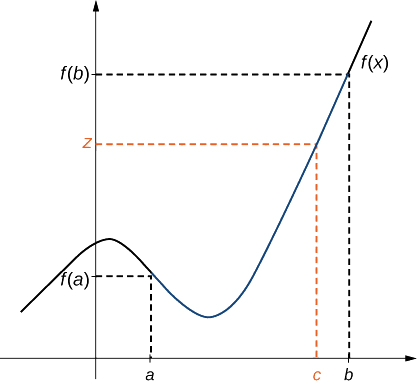
\includegraphics{img/2.4.3.png}

\begin{example}

Show that \(f(x)=x-\cos x\) has at least one zero.

\end{example}
\vspace*{6\baselineskip}

\subsection{Practice}





\begin{exercise}

  Using the definition, determine whether the function
  \(f(x)=\begin{cases}2x+1, & \text{if }x<1\\2, & \text{if }x=1\\ -x+4, & \text{if }x>1\end{cases}\)
  is continuous at \(x=1\). If the function is not continuous at 1,
  indicate the condition for continuity at a point that fails to hold.
  
  \end{exercise}
  \vspace*{6\baselineskip}
  
\begin{exercise}

Classify this discontinuity as removable, jump, or infinite.

\begin{enumerate}
\item
  Determine whether \(f(x)=\dfrac{x+2}{x+1}\) is continuous at \(-1\).
  If the function is discontinuous at \(-1\), classify the discontinuity
  as removable, jump, or infinite.
\item
  Determine whether
  \(f(x)=\begin{cases}x^2, &\text{if }x\ne 1\\3, & \text{if }x=1\end{cases}\)
  is continuous at \(1\). If \(f\) is not continuous at \(1\), classify
  the discontinuity as removable, jump, or infinite.
\item
  Determine whether the function
  \(f(x)=\begin{cases}-x+1, & \mathrm{if} \; x\le 2 \\ x^2-3, & \mathrm{if} \; x>2\end{cases}\)
  is continuous at \(x=2\). If \(f\) is not continuous at \(1\),
  classify the discontinuity as removable, jump, or infinite.
\end{enumerate}

\end{exercise}

\begin{exercise}

State the interval(s) over which the function
\(f(x)=\frac{x-1}{\sqrt{x+3}}\) is continuous.

\end{exercise}
\vspace*{6\baselineskip}

\begin{exercise}

Evaluate the limit \(\lim\limits_{x\to \frac\pi3}\tan(2\pi-3x)\).

\end{exercise}
\vspace*{6\baselineskip}

\begin{exercise}

Show that \(f(x)=x^3-x^2-3x+1\) has a zero over the interval \([0,1]\).

\end{exercise}
\vspace*{6\baselineskip}

\begin{exercise}

For \(f(x)=1/x,f(-1)=-1<0\) and \(f(1)=1>0\). Can we conclude that
\(f(x)\) has a zero in the interval \([-1,1]\)?

\end{exercise}


\newlecture
% !TeX root = main.tex

\hypertarget{defining-the-derivative}{%
\section{Defining the Derivative}\label{defining-the-derivative}}

\hypertarget{difference-quotient}{%
\subsection{Difference Quotient}\label{difference-quotient}}

Let \(f\) be a function defined on an interval \(I\) containing \(a\).
If \(x\neq a\) is in \(I\), then the \emph{difference quotient.} is \[
Q=\frac{f(x)-f(a)}{x-a}.
\] If \(h\neq 0\) is chosen so that \(a+h\) is in \(I\), then \[
Q=\frac{f(a+h)-f(a)}{a+h-a}=\frac{f(a+h)-f(a)}{h}
\] is a difference quotient with increment \(h\).

The slope of a tangent line is the limit of a difference quotient \[
m_{t a n}=\lim\limits_{x \to a} \frac{f(x)-f(a)}{x-a} .
\] Equivalently, \[
m_{\tan }=\lim\limits_{h \to 0} \frac{f(a+h)-f(a)}{h}
\]

\begin{figure}[h!]
\centering
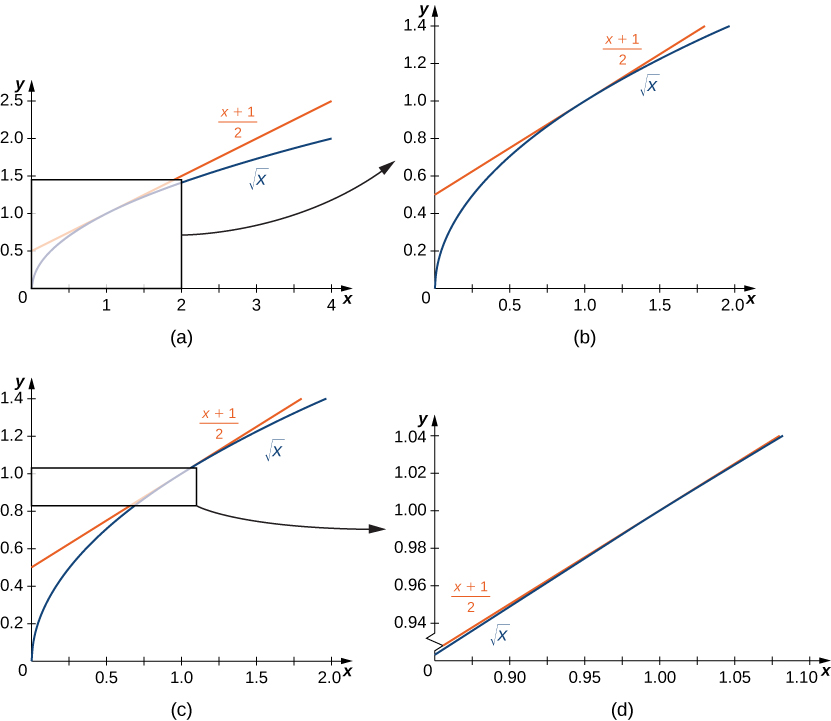
\includegraphics[width=\textwidth]{img/locally-linear.jpeg}
\par Smooth curves are locally linear
\end{figure}

\begin{example}
  Find the equation of the line tangent to the graph of  $f(x)=x^2$  at $x=3$.
\end{example}
\vspace*{6\baselineskip}

\hypertarget{derivative}{%
\subsection{Derivative}\label{derivative}}

\begin{definition}
  Let \(f\) be a function defined in an open interval
  containing \(a\). The \textbf{derivative of the function \(f(x)\) at
  \(a\)}, denoted by \(f'(a)\), is defined by \[
  f^{\prime}(a)=\lim\limits_{x \to a} \frac{f(x)-f(a)}{x-a}
  \] provided this limit exists.
  
  Alternatively, we may also define the derivative of \(f(x)\) at \(a\) as
  \[
  f^{\prime}(a)=\lim\limits_{h \to 0} \frac{f(a+h)-f(a)}{h}.
  \]
  
  The function \(f\) is said \textbf{differentiable} at \(a\) if the limit
  \(\lim\limits_{x \to a} \frac{f(x)-f(a)}{x-a}\) exists.  
\end{definition}

\begin{example}
For \(f(x)=x^2+3x+2\), find \(f'(1)\) using the definition of
derivative.
\end{example}
\vspace*{6\baselineskip}

\begin{example}
Find the line tangent to \(f(x)=\sqrt{x}\) at \(x=4\).
\end{example}
\vspace*{6\baselineskip}

\begin{example}
The following limit defines the derivative of a
function \(f\) at some number \(a\). Find the function \(f\) and
\(a\).\\
\[\lim\limits_{h\to 0}\dfrac{2(2+h)^2-8}{h}\]
\end{example}
\vspace*{6\baselineskip}

\begin{example}
Find the derivative of the following function at \(x=0\) if it exists.
\[
f(x)=\begin{cases}x^{2}\sin(1/x)&{\text{if }}x\neq 0\\0&{\text{if }}x=0\end{cases}
\]
\end{example}
\vspace*{6\baselineskip}

\hypertarget{instantaneous-rate-of-change}{%
\subsection{Instantaneous Rate of
Change}\label{instantaneous-rate-of-change}}

\begin{definition}
The \textbf{instantaneous rate of change} of a function \(f(x)\) at a
value \(a\) is its derivative \(f'(a)\).
\end{definition}

The \textbf{average velocity} is a rate of change \[
v_{ave}=\frac{s(t)-s(a)}{t-a}.
\] The \textbf{instantaneous velocity} is the limit of the average
velocity \[
v(a)=s^{\prime}(a)=\lim\limits_{t \to a} \frac{s(t)-s(a)}{t-a}
\]

\begin{example}
A rock is dropped from a height of 64 feet. Its height above ground at
time \(t\) seconds later is given by \(s(t)=-16t^2+64\),
\(0\le t\le 3\). Find its instantaneous velocity \(1\) second after it
dropped.
\end{example}
\vspace*{6\baselineskip}

\subsection{Practice}




\begin{exercise}
  Find the slope of the line tangent to the graph of  $f(x)=\sqrt{x}$ at $x=4$.
\end{exercise}
\vspace*{6\baselineskip}

\begin{exercise}
Find the tangent line to \(f(x)=\sin(x)\) at \(x=0\).
\end{exercise}
\vspace*{6\baselineskip}

\begin{exercise}
The following limit defines the derivative of a function \(f\) at some
number \(a\). Find the function \(f\) and \(a\).
\[\lim\limits_{h\to 0}\dfrac{4\sqrt[3]{8+h}-8}{h}\]
\end{exercise}
\vspace*{6\baselineskip}

\begin{exercise}
Determine whether the derivative of the following function at \(x=0\)
exists. \[
f(x)=\begin{cases}x\sin(1/x)&{\text{if }}x\neq 0\\0&{\text{if }}x=0\end{cases}
\]
\end{exercise}
\vspace*{6\baselineskip}

\begin{exercise}
  A coffee shop determines that the daily profit on scones obtained by charging s dollars per scone is  $P(s)=-20s^2+150s-10$. The coffee shop currently charges  \$3.25  per scone. Find  $P'(3.25)$, the rate of change of profit when the price is  \$3.25  and decide whether or not the coffee shop should consider raising or lowering its prices on scones.
\end{exercise}
\vspace*{6\baselineskip}

\begin{exercise}
Two particles traveling along straight lines side by side from start at
the same time. The graphs of their position functions \(f(t)\) and
\(g(t)\) are given below.

At time \(t=4\), which particle travels slower? Why?

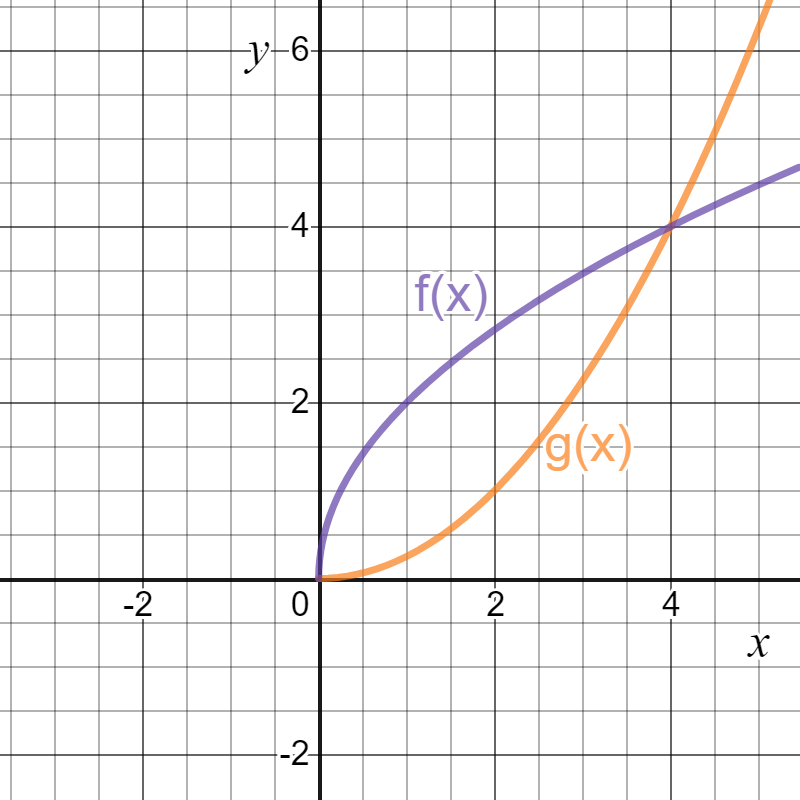
\includegraphics[width=0.8\textwidth]{img/desmos-two-functions.png}

\end{exercise}



\newlecture
% !TeX root = main.tex

\hypertarget{derivative-functions}{%
\section{Derivative Functions}\label{derivative-functions}}

\hypertarget{derivative-function---definition}{%
\subsection{Derivative Function -
Definition}\label{derivative-function---definition}}

\begin{definition}
Let \(f\) be a function. The \textbf{derivative function}, denoted by
\(f'\), is the function whose domain consists of those values of \(x\)
such that the following limit exists:
\[f'(x)=\lim_{h\to 0}\frac{f(x+h)-f(x)}{h}.\]

A function is said to be \textbf{differentiable over an open set} \(U\)
if it is differentiable at every point in $U$.

A function is called a \textbf{differential function} if it is
differentiable over its domain. At boundary points of the domain, the
differentiability is taken to be the left or right differentiability.
\end{definition}

\begin{example}
Determine whether the function \(f(x)=x^3\) is differentiable and find
the derivative function if it is differentiable.
\end{example}
\vspace*{6\baselineskip}

\begin{example}
Determine whether the function \(f(x)=\sqrt{x}\) is differentiable and
find the derivative function if it is differentiable.
\end{example}
\vspace*{6\baselineskip}

\hypertarget{notations-for-derivatives-and-differentiation}{%
\subsection{Notations for Derivatives and
Differentiation}\label{notations-for-derivatives-and-differentiation}}

When a function is given in the form \(y=f(x)\), we also use \(y'\) to
denote the derivative function. The notations \(f'\) and \(y'\) are
known as Lagrange's ``prime'' notation.

As the derivative function is essentially (the limit) a difference
quotient, we also use \(\frac{\mathrm{d}y}{\mathrm{d x}}\) (or
\(\mathrm{d}y/\mathrm{d x}\)) to denote the derivative functions. The
notation \(\frac{\mathrm{d}y}{\mathrm{d x}}\) was introduced by Leibniz
and called
\href{https://en.wikipedia.org/wiki/Leibniz\%27s_notation}{Leibniz's
notation}.

\begin{remark}
The notation \(\mathrm{d} x\) and \(\mathrm{d} y\) may be considered as
variables and are called \textbf{differentials}. Indeed,
\(\mathrm{d} x=x-a\) is the difference, by \(\mathrm{d}y = f'(a)(x-a)\)
is only an approximation of \(f(x)-f(a)\).
\end{remark}

The process of calculating a derivative is known as
\textbf{differentiation}. We view the prime \('\) or better the notation
\(\frac{\mathrm{d}}{\mathrm{d}x}\) as an operator and call it the
\textbf{differential operator}.

Sometimes, a differential operator is also denoted as \(D\) or \(D_x\)
to indicate the independent variable \(x\). Those notations are known as
Euler's notation.

\hypertarget{differentiability-implies-continuity}{%
\subsection{Differentiability implies
continuity}\label{differentiability-implies-continuity}}

\begin{theorem}
If the function \(f\) is differentiable at \(a\), then \(f\) is
continuous at \(a\).
\end{theorem}

\begin{remark}
\begin{enumerate}[sepno]
\item
  If a function is not continuous, it cannot be differentiable.
\item
  Not every continuous function is differentiable.
\end{enumerate}
\end{remark}

\begin{example}
(Continuous but not differentiable functions)

\begin{enumerate}
\item
  The function \(f(x)=|x|\) is continuous but failed to be
  differentiable at \(0\). Its graph has a sharp corner at \(0.\).
\item
  The function \(f(x)=\sqrt[3]{x}\) also fails to be differentiable at
  \(0\). Because it has a vertical tangent line at \(0\).
\item
  The function
\[f(x)=\begin{cases}x\sin\left(\frac{1}{x}\right),& \text{ if } x\ne 0\\0, & \text{ if } x=\end{cases}\]
is continuous but fails to be differentiable at a point in more
complicated ways.
\end{enumerate}
\end{example}
\vspace*{6\baselineskip}

\begin{example}
Find values of \(a\) and \(b\) that make the following function
differential. \[
f(x)=
\begin{cases}
    ax+ & x\ge 1\\
    x^2-3 & x<1\end{cases}
\]
\end{example}
\vspace*{6\baselineskip}

\hypertarget{higher-derivatives}{%
\subsection{Higher derivatives}\label{higher-derivatives}}

Higher derivatives are defined as repeated differentiations of
functions.

The \textbf{second derivative} \(f''(x)=(f'(x))'\) is defined the
derivative of the first derivative of \(f\).

The \textbf{third derivative} is defined as \(f'''(x)=(f''(x))'\).

The \textbf{\(n\)-th derivative} is defined recursively as
\(f^{(n)}(x)=(f^{(n-1)}(x))'\).

\begin{example}
Find the second derivative \(f''\) of the function \(f(x)=2x^2-3x+1\).
\end{example}
\vspace*{6\baselineskip}

\begin{example}
The position of a particle along a coordinate axis at time \(t\) (in
seconds) is given by \(s(t)=3t^2-4t+1\) (in meters). Find the function
that describes its acceleration at time \(t\).
\end{example}
\vspace*{6\baselineskip}

\subsection{Practice}

\begin{exercise}
  Determine whether the function \(f(x)=x^2-3x\) is differentiable and
  find the derivative function if it is differentiable.
  \end{exercise}
  \vspace*{6\baselineskip}
  
  \begin{exercise}
  Determine whether the function \(f(x)=\sqrt[3]{x}\) is differentiable
  and find the derivative function if it is differentiable.
  \end{exercise}
  \vspace*{6\baselineskip}
  
  \begin{exercise}
  Determine whether the function \(f(x)=\frac{1}{x+1}\) is differentiable
  and find the derivative function if it is differentiable.
  \end{exercise}
  \vspace*{6\baselineskip}
  
\begin{exercise}
Find values of \(a\) and \(b\) that make the following function
differentiable at \(x=3\).
\[f(x)=\begin{cases}ax+b, & \text{ if } x<3\\x^2,& \text{ if } x\ge \end{cases}\]
\end{exercise}
\vspace*{6\baselineskip}

\begin{exercise}
The position of a particle along a coordinate axis at time \(t\) (in
seconds) is given by \(s(t)=2t^3-3t^2+t\) (in meters). Find the function
that describes its acceleration at time \(t\).
\end{exercise}
\vspace*{6\baselineskip}



\newlecture
% !TeX root = main.tex

\hypertarget{rules-of-derivatives}{%
\section{Rules of Derivatives}\label{rules-of-derivatives}}

\hypertarget{basic-rules}{%
\subsection{Basic Rules}\label{basic-rules}}

\textbf{The Constant Rule:} Let \(c\) be a constant number. Then
\[\frac{\mathrm{d}}{\mathrm{d}\,x}(c)=0.\]

\textbf{The Power Rule:} Let \(n\) be a positive integer. Then
\[\dfrac{\mathrm{d}}{\mathrm{d}\,x}\left(x^n\right)=nx^{n-1}.\]

\begin{example}
Let \(f(x)=x^4\). Find \(f'(x)\).
\end{example}
\vspace*{6\baselineskip}

\hypertarget{linear-combination-rules}{%
\subsection{Linear Combination Rules}\label{linear-combination-rules}}

Let \(f\) and \(g\) be differentiable functions. Let \(a\) and \(b\) be
two constant numbers. Then \[\big(af+bg\big)'(x)=af'(x)+bg'(x).\]

\begin{example}
Let \(f(x)=4x^5-3x^2+7\). Find \(f'(x)\)
\end{example}
\vspace*{6\baselineskip}

\hypertarget{the-product-and-quotient-rules}{%
\subsection{The Product and Quotient
Rules}\label{the-product-and-quotient-rules}}

\textbf{Product Rule:} Let \(f\) and \(g\) be differentiable
functions. Then \[
(f\cdot g)'(x)=f'(x)g(x)+f(x)g'(x).
\]


\begin{example}
Find the derivative of the function \(f(x)=(x^3-2x+1)(x^2-3x+5)\).
\end{example}
\vspace*{6\baselineskip}

\begin{example}
For \(p(x)=f(x)g(x)\), use the product rule to find \(p'(2)\) if
\(f(2)=3,\; f'(2)=-4,\; g(2)=1\), and \(g'(2)=6\).
\end{example}
\vspace*{6\baselineskip}

\textbf{The Quotient Rule:} Let \(f\) and \(g\) be differentiable
functions. Then
\[\left(\dfrac{f}{g}\right)'(x)=\dfrac{f'(x)g(x)-f(x)g'(x)}{(g(x))^2}.\]

\begin{example}
Find the derivative of the function \(f(x)=\dfrac{x^2-3x}{3x-5}\).
\end{example}
\vspace*{6\baselineskip}

\begin{example}
Let \(f=\dfrac{g}{x^2+1}\) where the graph of the function \(g\) is
given below. Find \(f'(2)\).\\
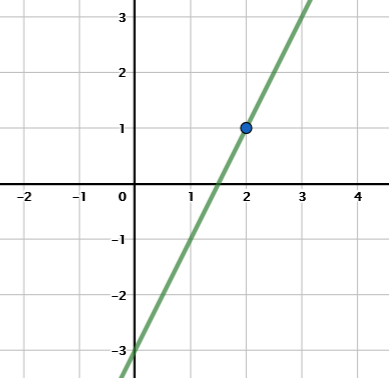
\includegraphics[width=0.8\textwidth]{img/quotientRuleLinear.png}
\end{example}
\vspace*{6\baselineskip}

\hypertarget{extended-power-rule}{%
\subsection{Extended Power Rule}\label{extended-power-rule}}

Let \(k\) is a real number. Then
\[\dfrac{\mathrm{d}}{\mathrm{d}\,x}(x^k)=kx^{k-1}.\]

If \(k\) is a negative integer, the formula follows from the quotient
rule. The proof of the general cases has to be postponed after
logarithmic and exponential functions in Calculus II.

\begin{example}
Find \(\dfrac{\mathrm{d}}{\mathrm{d}\,x}(x^{-5})\).
\end{example}
\vspace*{6\baselineskip}

\begin{example}
Find \(\dfrac{\mathrm{d}}{\mathrm{d}\,x}\dfrac{1}{\sqrt[3]{x}}\).
\end{example}
\vspace*{6\baselineskip}

\hypertarget{example-and-practice-on-differentiation-rules}{%
\subsection{More Examples and Practice}\label{example-and-practice-on-differentiation-rules}}

\begin{example}
Let \(f(x)=3x^2h(x)+\dfrac{g(x)}{x}\). Find \(f'(x)\) in terms of \(h\),
\(g\), \(h'\) and \(g'\).
\end{example}
\vspace*{6\baselineskip}

\begin{example}
Determine the values of \(x\) for which \(f(x)=x^3-7x^2+8x+1\) has a
horizontal tangent line.
\end{example}
\vspace*{6\baselineskip}

\begin{example}
Find equations of the normal line to the curve \(y=4\sqrt{x}-x\) at
\((1,3)\).
\end{example}
\vspace*{6\baselineskip}

\subsection{Practice}

\begin{exercise}
  Let \(f(x)=x^{11}\). Find \(f'(x)\).
  \end{exercise}
  \vspace*{6\baselineskip}
  
\begin{exercise}
Let \(g(x)=5x^{10}-5x^3-9\). Find \(g'(x)\).
\end{exercise}
\vspace*{6\baselineskip}

\begin{exercise}
Find the equation of the line tangent to the graph of \(f(x)=x^2-4x+6\)
at \(x=1\).
\end{exercise}
\vspace*{6\baselineskip}

\begin{exercise}
Let \(h(x)=f(x)(x^3-3x^2-2x)\) where \(f\) is differentiable, \(f(1)=2\)
and \(f'(1)=3\). Find \(h'(1)\).
\end{exercise}
\vspace*{6\baselineskip}

\begin{exercise}
Find \(h'(x)\) for \(h(x)=\dfrac{1}{x^5}\).
\end{exercise}
\vspace*{6\baselineskip}

\begin{exercise}
Let \(f\) and \(g\) be differentiable functions such that \(f(3)=2\),
\(f'(3)=-1\), \(g(3)=-2\) and \(g'(3)=1\). Find the \(h'(3)\) where
\(h(x)=\dfrac{f(x)-2}{g(x)}\).
\end{exercise}
\vspace*{6\baselineskip}

\begin{exercise}
Find the derivative of the function \(f(x)=\dfrac{1}{\sqrt[7]{x^3}}\).
\end{exercise}
\vspace*{6\baselineskip}

\begin{exercise}
  Find \(g'(x)\) for
  \(g(x)=\frac{3x^2+5x-7}{\sqrt{x}}\).
\end{exercise}
\vspace*{6\baselineskip}

\begin{exercise}
Let \(h(x)=\dfrac{2x^3f(x)}{3x+g(x)}\). Find \(h'(x)\) in terms of
\(f\), \(g\), \(f'\) and \(g'\).
\end{exercise}
\vspace*{6\baselineskip}

\begin{exercise}
Determine the values of \(x\) for which \(f(x)=2x^3-5x^2-x+7\) has a
tangent line parallel to \(y=3x-1\).
\end{exercise}
\vspace*{6\baselineskip}

\begin{exercise}
Suppose that \(f\) and \(g\) are both differentiable functions with
\(f(4)=3\), \(g(4)=2\), \(f'(4)=9\) and \(g'(4)=5\). Find \(h'(4)\)
where \[
h(x)=\frac{2}{\sqrt{x}}-\frac{f(x)-1}{g(x)}.
\]
\end{exercise}



\newlecture
% !TeX root = main.tex

\hypertarget{derivatives-of-trigonometric-functions}{%
\section{Derivatives of Trigonometric
Functions}\label{derivatives-of-trigonometric-functions}}

\hypertarget{the-derivative-of-the-sine-function}{%
\subsection{The Derivative of the Sine
Function}\label{the-derivative-of-the-sine-function}}

Recall the formula of sum of angles 
\[
\begin{aligned}
  \sin(x+h)=&\sin x\cos h+\cos x\sin h\\[0.5em]
  \cos(x+h)=&\cos x\cos h-\sin x\sin h.
\end{aligned}
\] Then for any \(x\), we have \[
\begin{aligned}
  \dfrac{\mathrm{d}}{\mathrm{d} x}(\sin x)=&\lim\limits_{h\to 0}\dfrac{\sin(x+h)-\sin x}{h}\\
  =&\lim\limits_{h\to 0}\dfrac{\sin x\cos h+\cos x\sin h-\sin x}{h}\\
  =&\lim\limits_{h\to 0}\dfrac{\sin x(\cos h-1)}{h}+\lim\limits_{h\to 0}\dfrac{\cos x\sin h}{h}\\
  =&\sin x\lim\limits_{h\to 0}\dfrac{\cos h-1}{h}+\cos x\lim\limits_{h\to 0}\dfrac{\sin h}{h}\\
  =&\sin x\cdot 0 +\cos x\cdot 1\\
  =&\cos x.
\end{aligned}
\]

\begin{example}

Find the derivative of \(f(x)=x^2\sin x\).

\end{example}
\vspace*{6\baselineskip}

\hypertarget{derivatives-of-other-trigonometric-functions}{%
\subsection{Derivatives of Other Trigonometric
Functions}\label{derivatives-of-other-trigonometric-functions}}

Using the sum angle formula for cosine and limit laws of quotients, we
obtain the following formulas of derivative of trigonometric functions.
\[
\begin{aligned}
\dfrac{\mathrm{d}}{\mathrm{d} x}\sin x &= \cos x \\
\dfrac{\mathrm{d}}{\mathrm{d} x}\cos x &= -\sin x\\
\dfrac{\mathrm{d}}{\mathrm{d} x}\tan x &= \sec^2x\\
\end{aligned}
\qquad
\begin{aligned}
\dfrac{\mathrm{d}}{\mathrm{d} x}\csc x &= -\csc x \cot x \\
\dfrac{\mathrm{d}}{\mathrm{d} x}\sec x &= \sec x\tan x\\
\dfrac{\mathrm{d}}{\mathrm{d} x}\cot x &= -\csc^2x\\
\end{aligned}
\]

\begin{example}

Find the derivative of \(f(x)=\cos x\sin x\).

\end{example}
\vspace*{6\baselineskip}

\begin{example}

Find the derivative of \(f(x)=\dfrac{\cos x-1}{\sin x+1}\).

\end{example}
\vspace*{6\baselineskip}

\begin{example}

Find the derivative of \(f(x)=2x\tan x-3\cot x\).

\end{example}
\vspace*{6\baselineskip}

\begin{example}

Find the derivative of \(f(x)=\sec^2x-x\csc x\).

\end{example}
\vspace*{6\baselineskip}

\begin{example}

Find the 59-th derivative
\(\dfrac{\mathrm{d}^{59}}{\mathrm{d}x^{59}}(\sin x)\).

\end{example}
\vspace*{6\baselineskip}

\subsection{Practice}

\begin{exercise}

  Find the derivative of \(f(x)=\dfrac{x^3+x}{\sin x}\).
  
  \end{exercise}
  \vspace*{6\baselineskip}
  
\begin{exercise}

Find the derivative of \(f(x)=\dfrac{\sin x+\cos x}{\sin x-\cos x}\).

\end{exercise}
\vspace*{6\baselineskip}

\begin{exercise}

Find the derivatives of the function \(f(x)=3\tan x+\sqrt{x^5}\).

\end{exercise}
\vspace*{6\baselineskip}

\begin{exercise}

Find the derivative of \(f(x)=(x+\tan x)(\sec x + x^2)\).

\end{exercise}
\vspace*{6\baselineskip}

\begin{exercise}

Find the 3-th derivative
\(\dfrac{\mathrm{d}^{3}}{\mathrm{d}x^{3}}(\tan x)\).

\end{exercise}
\vspace*{6\baselineskip}



\newlecture
% !TeX root = main.tex

\hypertarget{the-chain-rule}{%
\section{The Chain Rule}\label{the-chain-rule}}

If \(y=f(u)\) and \(u=g(x)\) are differentiable functions, intuitively,
using Leibniz's notation, you may find \[
\frac{\mathrm{d} y}{\mathrm{d} x}=\frac{\mathrm{d} y}{\mathrm{d} u}\cdot\frac{\mathrm{d} u}{\mathrm{d} x}.
\]

This identity is indeed true and called the Chain Rule which is one of
the most important of the differentiation rules.

\begin{theorem}

If \(g\) is differentiable at \(x\) and \(f\) is differentiable at
\(g(x)\), then the composite function \(F=f\circ g\) defined by
\(F(x)=f(g(x))\) is differentiable at \(x\) and \[
F'(x)=f'(g(x))\cdot g'(x).
\]

\end{theorem}

In the chain rule, \(f'(g(x))\) mean the ``output'' of the derivative
function \(f'\) for the ``input'' \(g(x)\).

The theorem can be proved using the error function of an estimation. Let
\(\varepsilon(t)=\frac{f(u+t)-f(u)}{t}-f'(u)\) and \(k=g(x+h)-g(x)\).
Then \[
\begin{aligned}
  \dfrac{f(g(x+h))-f(g(x))}{h}
  =&\dfrac{f(g(x)+k)-f(g(x))}{h}\\
  =&\frac{k(\varepsilon(k)+f'(g(x))}{h}.
\end{aligned}
\] Taking limits will give the chain rule formula.

\begin{example}

\textbf{(General Power Rule):} Let \(f\) be a function differentiable at
\(x\) and \(h(x)=(f(x))^n\). Find \(h'(x)\).

\end{example}
\vspace*{6\baselineskip}

\begin{example}

Find the derivative of \(f(x)=\dfrac{1}{(x+1)^3}\).

\end{example}
\vspace*{6\baselineskip}

\begin{example}

Find the derivative of \(f(x)=\sin(\dfrac{\pi}{2}-x)\).

\end{example}
\vspace*{6\baselineskip}

\begin{example}

Find the derivative of \(f(x)=\tan(\cos x+1)\).

\end{example}
\vspace*{6\baselineskip}

\begin{example}

Find the derivative of \(f(x)=\dfrac{x}{(2x+1)^3}\).

\end{example}
\vspace*{6\baselineskip}

\begin{example}
  Find the derivative
  \(\dfrac{\mathrm{d}}{\mathrm{d}x}\left(\dfrac{1}{\sqrt{1+\sin(x^2+1)}}\right)\).
\end{example}
\vspace*{6\baselineskip}

\begin{example}

Find all points on the curve \(y=\cos x-\cos^2x\) at which the tangent
line is horizontal.

\end{example}
\vspace*{6\baselineskip}

\subsection{Practice}

\begin{exercise}

Find the derivative of \(y=\sqrt{x^2+5}\).

\end{exercise}
\vspace*{6\baselineskip}

\begin{exercise}

Find the derivative \(\dfrac{\mathrm{d}}{\mathrm{d}x}\cos(u+1)\) where
\(u=x^3\).

\end{exercise}
\vspace*{6\baselineskip}

\begin{exercise}

Find the derivatives of the function
\(f(x)=\sqrt{\frac{(x+1)(x-2)}{(x-1)(x+2)}}\).

\end{exercise}
\vspace*{6\baselineskip}

\begin{exercise}

Find all points on the curve \(y=\sqrt{4x+1}\) at which the tangent line
is parallel to the line \(2x-y=1\).

\end{exercise}
\vspace*{6\baselineskip}



\newlecture
% !TeX root = main.tex

\hypertarget{implicit-differentiation}{%
\section{Implicit Differentiation}\label{implicit-differentiation}}

As an application of the chain rule, the technique of \textbf{implicit
differentiation} allows us to find the derivative of an implicitly
defined function without ever solving for the function explicitly.

\textbf{Problem-Solving Strategy: Implicit Differentiation}

\begin{enumerate}[sepno]
\item
  Take the derivative of (or differentiate)both sides of the equation.
  Keep in mind that \(y\) is a function of \(x\).
\item
  Solve for \(y'\) (or \(\dfrac{\mathrm{d}y}{\mathrm{d}x}\)) from the
  resulting equation.
\end{enumerate}

\begin{example}

Find \(\dfrac{\mathrm{d}y}{\mathrm{d}x}\) where \(y\) is a function of
\(x\) defined by the equation \(x^3+y^2=1\).

\end{example}
\vspace*{6\baselineskip}

\begin{example}

Find \(\dfrac{\mathrm{d}y}{\mathrm{d}x}\) where \(y\) is a function of
\(x\) defined by the equation \(2\sin x-1=\cos y\).

\end{example}
\vspace*{6\baselineskip}

\begin{example}

Find \(\dfrac{\mathrm{d}y}{\mathrm{d}x}\) for the function \(y\)
implicitly defined by the equation \(x^3\sin y+\tan y=3x+2\).

\end{example}
\vspace*{6\baselineskip}

\begin{example}

Find \(\dfrac{\mathrm{d}^2y}{\mathrm{d}x^2}\) given that \(y\) is
implicitly defined by \(x^2-y^2=15\).

\end{example}
\vspace*{6\baselineskip}

\begin{example}

Find the equations of lines tangent to the curve
\(2xy=\dfrac xy+\dfrac yx\) at the point (1,1).

\end{example}
\vspace*{6\baselineskip}

\begin{example}

The number of cars produced when \(x\) dollars is spent on labor and
\(y\) dollars is spent on capital invested by a manufacturer can be
modeled by the equation \(\displaystyle 40x^{\frac13} y^{\frac23}=480\).

\begin{enumerate}
\item
  Find a formula in terms of \(x\) and \(y\) for
  \(\displaystyle \frac{\mathrm{d}{y}}{\mathrm{d}{x}}\). \hspace{0pt}
\item
  Find the value of of
  \(\displaystyle \frac{\mathrm{d}{y}}{\mathrm{d}{x}}\) at the point
  (27,8).
\end{enumerate}

\end{example}

\begin{example}

Find all points \((x,y)\) on the graph of the equation
\(2x^2 + 8y^2= x + 4 y\) such that \(x>0\), \(y>0\) and at where the
tangent line is

\begin{enumerate}
\item
  horizontal
\item
  vertical
\end{enumerate}

\end{example}

\subsection{Practice}

\begin{exercise}

Find \(y'\) where \(y\) is a function of \(x\) defined implicitly by the
equation \(x^2-xy+y^2=1\).

\end{exercise}
\vspace*{6\baselineskip}

\begin{exercise}

Find \(\dfrac{\mathrm{d}y}{\mathrm{d}x}\) for \(y\) defined implicitly
by the equation \(x^2\cos y+y^2=3x+1\).

\end{exercise}
\vspace*{6\baselineskip}

\begin{exercise}

Find the \(\dfrac{\mathrm{d}^2y}{\mathrm{d}x^2}\) where \(y\) is a
function defined implicitly by the equation \(x^3+y^2=3x+1\).

\end{exercise}
\vspace*{6\baselineskip}

\begin{exercise}

Find the equation of the line tangent to the graph of \(y^3+x^3 - 3xy=0\)
at the point \((\frac32,\frac32)\).

\end{exercise}
\vspace*{6\baselineskip}

\begin{exercise}

Find all points \((x,y)\) on the graph of the equation
\(2x^2 + 8y^2= x + 4 y\) such that \(x>0\), \(y>0\) and at where the
tangent line is

\begin{enumerate}
\item
  horizontal
\item
  vertical
\end{enumerate}

\end{exercise}



\newlecture
% !TeX root = main.tex

\hypertarget{derivatives-as-rates-of-change}{%
\section{Derivatives as Rates of
Change}\label{derivatives-as-rates-of-change}}

If \(f(x)\) is a function defined on a small interval \([a, a+h]\), then
the amount of change of \(f(x)\) over the interval \(f(a+h)-f(a)\) is
approximately \(f'(a)h\) if \(f\) is differentiable at \(a\). This is
because
\[\lim\limits_{h\to 0}h\cdot\left(\dfrac{f(a+h)-f(a)}{h}-f'(a)\right)=0\]
which means \(f(a+h)-f(a)-f'(a)h\) can be arbitrarily small as long as
\(h\) is small enough.

\begin{fullwidth}
  \centering
  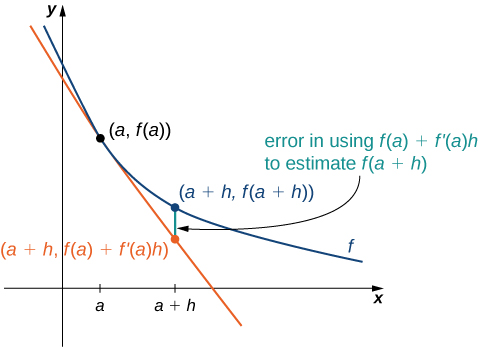
\includegraphics{img/DerivativeRateChange.png}
\end{fullwidth}

\hypertarget{motion-along-a-line}{%
\subsection{Motion Along a Line}\label{motion-along-a-line}}

\textbf{Definition:} Suppose an object is moving along a coordinate
line. Let \(s(t)\) be a function giving the position of the object at
time \(t\).

\begin{itemize}
\item
  The \textbf{displacement} of the object over the time interval from
  \(t\) to \(t+\Delta t\) is \(\Delta s=s(t+\Delta t)+s(t)\), where
  \(\Delta t\) is an increment of time.
\item
  The \textbf{average velocity} of the object over a time interval from
  \(t\) to \(t+\Delta t\) is \(v_{ave}=\dfrac{\Delta s}{\Delta t}\).
\item
  The \textbf{velocity (instantaneous velocity)} of the object at time
  \(t\) is given by
  \(v(t)=\lim\limits_{\Delta t\to 0}\dfrac{\Delta s}{\Delta t}=s'(t)\).
\item
  The \textbf{speed} of the object at time \(t\) is given by \(|v(t)|\).
\item
  The \textbf{acceleration} of the object at \(t\) is given by
  \(a(t)=v'(t)=s''(t)\).
\end{itemize}

\begin{example}

A ball is dropped from a height of 64 feet. Its height above ground (in
feet) \(t\) seconds later is given by \(s(t)=-16t^2+64\).

\begin{enumerate}
\item
  What is the velocity of the ball when it hits the ground?
\item
  When is the object at rest?
\end{enumerate}

\end{example}
% \vspace*{6\baselineskip}

\begin{example}

A particle moves along a coordinate axis. Its position at time \(t\) is given by
\(s(t)=t^3-9t^2+24t+4\).

\begin{enumerate}
\item
  Find \(v(t)\) and \(a(t)\) and use these values to answer the
  following questions.
\item
  On what time intervals is the particle moving from left to right?
\item
  On what time intervals is the particle moving from right to left?
\end{enumerate}

\end{example}
% \vspace*{6\baselineskip}

\hypertarget{population-change}{%
\subsection{Population Change}\label{population-change}}

\begin{definition}

If \(P(t)\) is the number of entities present in a population, then the
\textbf{population growth rate} of \(P(t)\) is defined to be \(P'(t)\).

\end{definition}

\begin{example}

The population of a city is tripling every 5 years. If its current
population is 10,000, what will be its approximate population 2 years
from now?

\end{example}
\vspace*{6\baselineskip}

\hypertarget{derivative-in-economics}{%
\subsection{Derivative in Economics}\label{derivative-in-economics}}

\begin{itemize}
\item
  If \(C(x)\) is the cost of producing \(x\) items, then the
  \textbf{marginal cost} \(MC(x)\) is \(MC(x)=C'(x)\).
\item
  If \(R(x)\) is the revenue obtained from selling \(x\) items, then the
  \textbf{marginal revenue} \(MR(x)\) is \(MR(x)=R'(x)\).
\item
  If \(P(x)=R(x)-C(x)\) is the profit obtained from selling \(x\) items,
  then the \textbf{marginal profit} \(MP(x)\) is defined to be
  \(MP(x)=P'(x)=MR(x)-MC(x)=R'(x)-C'(x)\).
\end{itemize}


\begin{example}

Suppose that the profit obtained from the sale of \(x\) fish-fry dinners is given by \(P(x)=-0.03x^2+8x-50\). Use the marginal profit function to estimate the profit from the sale of the 101st fish-fry dinner.

\end{example}
\vspace*{6\baselineskip}

\subsection{Practice}

\begin{exercise}
  A particle moves along a coordinate axis. Its position at time  t  is given by $s(t)=t^2-5t+1$ . Is the particle moving from right to left or from left to right at time  $t=3$?
\end{exercise}
\vspace*{6\baselineskip}

\begin{exercise}

  A particle moves along a coordinate axis. Its position at time \(t\) is given by
  \(s(t)=t^3-8t\).
  
  \begin{enumerate}
  \item
    Determine the direction the particle is traveling when $s(t)=0$.
  \item
    On what time intervals is the particle moving from right to left?
  \item
    Determine the direction the train is traveling when $a(t)=0$?
  \end{enumerate}
  
\end{exercise}


\begin{exercise}

The current population of a mosquito colony is known to be 3,000; that
is, \(P(0)=3,000\). If \(P'(0)=100\), estimate the size of the
population in 3 days, where \(t\) is measured in days.

\end{exercise}
\vspace*{6\baselineskip}

\begin{exercise}

The cost (in dollars) of producing \(x\) units of a certain commodity is
\(C(x) = 20 + 100\sqrt{x} + 0.01x^2\).

\begin{enumerate}
\item
  Find the marginal cost function.
\item
  Find \(C'(100)\) and explain it meaning.
\item
  What is the difference between \(C'(100)\) and the additional cost for
  producing the 1001st commodity?
\end{enumerate}

\end{exercise}



\newlecture
% !TeX root = main.tex

\hypertarget{related-rates}{%
\section{Related Rates}\label{related-rates}}

In many real-world applications, related variables are changing with
respect to a same variable. For example, the volume \(V\) and height
\(h\) of water in a cylindrical tank change with respect to time \(t\).
Such two rates of change, for example,
\(\dfrac{\mathrm{d}V}{\mathrm{d}t}\) and
\(\dfrac{\mathrm{d}h}{\mathrm{d}t}\) are called \textbf{related rates}.

To solve a related rate problem, the following strategy will be helpful.

\textbf{Problem-Solving Strategy: Solving a Related-Rates Problem}

\begin{enumerate}[sepno]
\item
  Assign symbols to all variables involved in the problem. Draw a figure
  if applicable.
\item
  State, in terms of the variables, the information that is given and
  the rate to be determined.
\item
  Find an equation relating the variables introduced in step 1.
\item
  Using the chain rule, differentiate both sides of the equation found
  in step 3 with respect to the independent variable. This new equation
  will relate the derivatives.
\item
  Substitute all known values into the equation from step 4, then solve
  for the unknown rate of change.
\end{enumerate}

\begin{example}

A \(13\)-ft ladder is leaning against a wall. If the bottom of the
ladder slides away from the wall at a rate \(2\) ft/min, how fast is the
top of the ladder slides down the wall when the bottom of the ladder is
\(12\) ft from the wall.

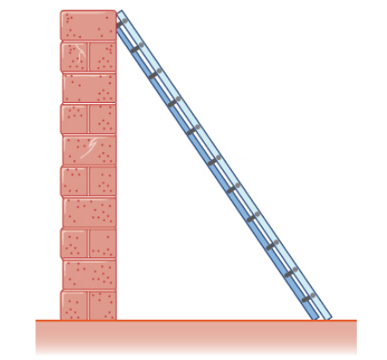
\includegraphics[scale=0.5]{img/image-20201007131231366.png}

\end{example}
\vspace*{6\baselineskip}

\begin{example}

A \(6\)-ft-tall person walks away from a \(10\)-ft lamppost at a
constant rate of \(3\) ft/sec.~What is the rate that the tip of the
shadow moves away from the pole when the person is \(10\) ft away from
the pole?

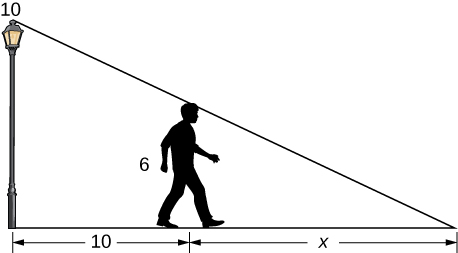
\includegraphics[scale=0.8]{img/CNX_Calc_Figure_04_01_203.jpeg}

\end{example}
\vspace*{6\baselineskip}

\begin{example}

A rocket is launched so that it rises vertically. A camera is positioned
\(5000\) ft from the launch pad. When the rocket is \(1000\) ft above the launch pad, 
its velocity is \(600\) ft/sec. Find the necessary rate of change of the camera's angle 
as a function of time so that it stays focused on the rocket.

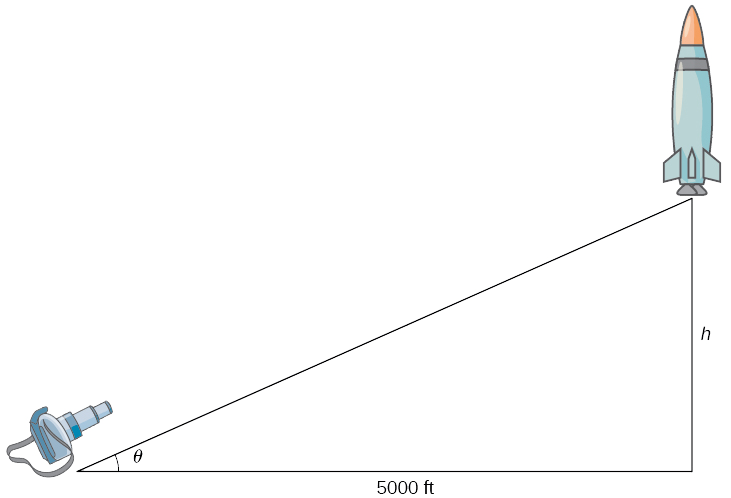
\includegraphics[scale=0.6]{img/4.1.3.png}

\end{example}
\vspace*{6\baselineskip}

\begin{example}

The altitude of a triangle is increasing at a rate of \(1.5\)
centimeters/minute while the area of the triangle is increasing at a
rate of \(5\) square centimeters/minute. At what rate is the base of the
triangle changing when the altitude is \(11\) centimeters and the area
is \(85\) square centimeters?

\end{example}
\vspace*{6\baselineskip}

\begin{example}

A trough has ends shaped like isosceles triangles, with width \(3\) m
and height \(4\) m, and the trough is \(10\) m long. Water is being
pumped into the trough at a rate of \(5\,\text{m}^3\text{/min}\). At
what rate does the height of the water change when the water is \(1\) m
deep?

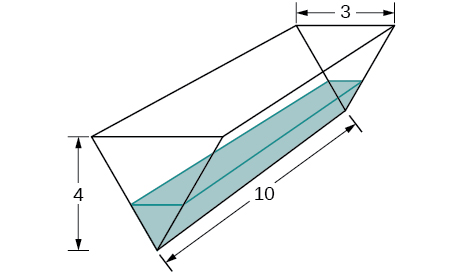
\includegraphics[scale=0.8]{img/CNX_Calc_Figure_04_01_204.jpeg}

\end{example}
\vspace*{6\baselineskip}

\begin{example}

Consider an inverted right cone that is leaking water. (Inverted means the cone's point is facing down, like a funnel.) The dimensions of the conical tank are a height of 16 ft and a radius of 5 ft.

Find the rate at which the surface area of the water changes when the
water is \(10\) ft high if the cone leaks water at a rate of
\(10 \,\text{ft}^3\text{/min}\).

\end{example}
\vspace*{6\baselineskip}

\subsection{Practice}

\begin{exercise}

The volume of a cube decreases at a rate of \(10\) m/sec. Find the rate
at which the side of the cube changes when the side of the cube is \(2\)
m.

\end{exercise}
\vspace*{6\baselineskip}

\begin{exercise}

An airplane is flying overhead at a constant elevation of \(4000\) ft. A
man is viewing the plane from a position \(3000\) ft from the base of a
radio tower. The airplane is flying horizontally away from the man. If
the plane is flying at the rate of \(600\) ft/sec, at what rate is the
distance between the man and the plane increasing when the plane passes
over the radio tower?

\end{exercise}
\vspace*{6\baselineskip}

\begin{exercise}

Two airplanes are flying in the air at the same height: airplane A is
flying east at \(250\) mi/h and airplane B is flying north at \(300\)
mi/h. If they are both heading to the same airport, located \(30\) miles
east of airplane A and \(40\) miles north of airplane B, at what rate is
the distance between the airplanes changing?

\end{exercise}
\vspace*{6\baselineskip}

\begin{exercise}

A circle is inside a square. The radius of the circle is decreasing at a
rate of \(4\) meters per minute and the sides of the square are
increasing at a rate of \(2\) meters per minute. When the radius is
\(4\) meters, and the sides are \(20\) meters, then how fast is the AREA
outside the circle but inside the square changing?

\end{exercise}
\vspace*{6\baselineskip}

\begin{exercise}

A rotating light is located \(14\) feet from a wall. The light completes
one rotation every \(5\) seconds. Find the rate at which the light
projected onto the wall is moving along the wall when the light's angle
is \(15\) degrees from perpendicular to the wall.

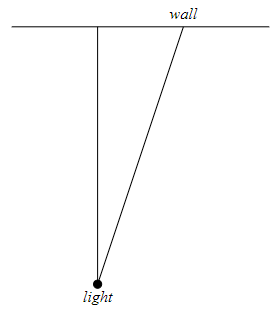
\includegraphics[scale=0.5]{img/image-20201007133107751.png}

\end{exercise}
\vspace*{6\baselineskip}

\begin{exercise}

A cylinder is leaking water but you are unable to determine at what
rate. The cylinder has a height of \(2\) m and a radius of \(2\) m. Find
the rate at which the water is leaking out of the cylinder if the rate
at which the height is decreasing is \(10\) cm/min when the height is
\(1\) m.

\end{exercise}



\newlecture
% !TeX root = main.tex

\hypertarget{linearization}{%
\section{Linearization}\label{linearization}}

Let \(f\) be a function differentiable at \(x=a\). Then for a number
\(x\) near \(a\), the value of the function \(f(x)\) can be approximated
using the tangent line \(y=f'(a)(x-a)+f(a)\).

That is \[f(x)\approx f'(a)(x-a)+f(a)\] We call the function
\(L(x):=f'(a)(x-a)+f(a)\) the \textbf{\emph{linearization}} or
\textbf{\emph{linear approximation}} of \(f\) at \(a\).

\begin{example}

Find the linearization of \(f(x)=\sqrt{x}\) at \(x=1\) and estimate
\(f(1.01)\). \url{https://www.desmos.com/calculator/urjragsxae}

\end{example}
\vspace*{6\baselineskip}

\begin{example}

Find the linearization of \(f(x)=\cos x\) at \(x=60^\circ\) and estimate
\(\cos(61^\circ)\).

\end{example}
\vspace*{6\baselineskip}

\begin{example}

Estimate the value of \(\sqrt[3]{0.98}\) using local linear
approximation for the function \(f(x)=\sqrt[3]{1+x}\).

\end{example}
\vspace*{6\baselineskip}

\hypertarget{differentials}{%
\subsection{Differentials}\label{differentials}}

Sometimes, we only need to know the relative change. The linear
approximation provides an estimate of the relative change in the
dependent variable \(y\) using the relative change of the independent
variable \(x\). Suppose that \(y=f(x)\). We denote by \(\mathrm{d}x\)
the change in \(x\) which can be assigned with any value, and define
\[\mathrm{d}y=f'(x)\mathrm{d}x.\] Then \(\mathrm{d}y\) can be viewed as
a function of \(\mathrm{d}x\). We call \(\mathrm{d}x\) and
\(\mathrm{d}y\) \textbf{\emph{differentials}}.

Given that \(f\) is differentiable at \(a\) and \(\mathrm{d}x\) is
small, the value \(f(a+\mathrm{d}x)\) is approximately

\[
f(a+\mathrm{d}x)\approx L(a+\mathrm{d}x)=f(a)+f'(a)(a+\mathrm{d}x - a).
\]

Then the actual change \(\Delta y=f(a+\mathrm{d}x)-f(a)\) is
approximately

\[
\Delta y=f(a+\mathrm{d}x) - f(a)\approx L(a+\mathrm{d}x) - f(a)=f'(a)\mathrm{d}x=dy.
\]

\begin{fullwidth}
  \centering
  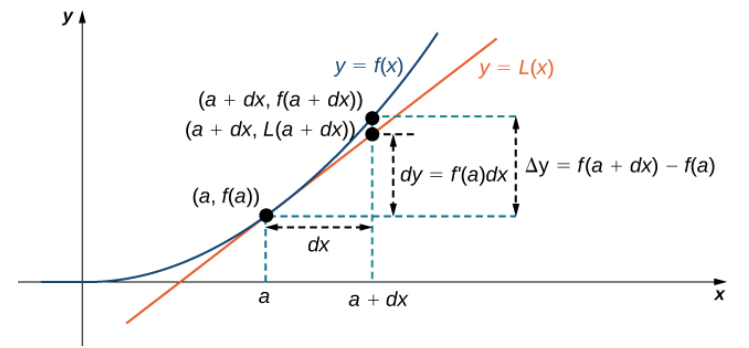
\includegraphics[scale=0.5]{img/image-20201017200202969.png}
\end{fullwidth}

\begin{example}

Find the differential \(\mathrm{d}y\) for the function \(y=x^3-\frac1x\)
and evaluate for \(x=1\) and \(\mathrm{d}x=0.01\).

\end{example}
\vspace*{6\baselineskip}

\begin{example}

Let \(y=tan(5x+2)\). Using the differential to estimate \(\Delta y\)
when \(x=1\) and \(\mathrm{d}x=0.4\).

\end{example}
\vspace*{6\baselineskip}

\hypertarget{applications-and-measurement-errors}{%
\subsection{Applications and Measurement
Errors}\label{applications-and-measurement-errors}}

In application, due errors in measurement, if a quantity is calculated
based on a measurement, it is likely subject to an error too. This type
of error is known as a \textbf{propagated error}. Suppose the quantity
is determined by a function \(f\) of the measurement \(x\). If the
measurement has an error \(\mathrm{d}x\), then the propagated error
\(f(a+\mathrm{d}x)-f(a)\) is approximately \[
\Delta y=f(a+\mathrm{d}x)-f(a)\approx f'(a)\mathrm{d}x=dy.
\]

\begin{remark}

\begin{remark}

When \(f'(x)\) is continuous, if we don't know \(a\), by continuity, we
may the measured value \(a+\mathrm{d}x,\) to estimate the propagated
error

\[
\Delta y\approx dy\approx f'(a+\mathrm{d}x)\mathrm{d}x.
\]

\end{remark}

\end{remark}

\begin{example}

Suppose the side length of a cube is measured to be 2 cm with an
accuracy of 0.1 cm.

\begin{enumerate}
\item
  Use differentials to estimate the error in the computed volume of the
  cube.
\item
  Compute the volume of the cube if the side length is (a) 1.9 cm and
  (b) 2.1 cm to compare the estimated error with the actual potential
  error.
\end{enumerate}

Given an absolute error \(\Delta q\) for a particular quantity, we
define the relative error as \(\frac{\Delta q}{q}\), where \(q\) is the
actual value of the quantity.

\end{example}

\begin{example}

An astronaut using a camera measures the radius of Earth as 4000 mi with
an error of \(\pm 80\) mi. Let's use differentials to estimate the relative
and percentage error of using this radius measurement to calculate the
volume of Earth, assuming the planet is a perfect sphere.

\end{example}
\vspace*{6\baselineskip}

\subsection{Practice}

\begin{exercise}

Find the linearization of \(f(x)=\sqrt[3]{x}\) at \(x=8\) and estimate
\(f(8.03)\).

\end{exercise}
\vspace*{6\baselineskip}

\begin{exercise}

Find the linearization of \(f(x)=\sec x\) at \(x= 45^\circ\) and
estimate \(f(44^\circ)\).

\end{exercise}
\vspace*{6\baselineskip}

\begin{exercise}

Find \(\mathrm{d}y\) for \(y=\sqrt[n]{x+1}\) and evaluate when \(x=0\)
and \(\mathrm{d}x=0. 01\), where \(n\) is a positive integer.

\end{exercise}
\vspace*{6\baselineskip}

\begin{exercise}

Find \(\mathrm{d}y\) for \(y=\sin\left(\dfrac{\pi x+\pi}{2}\right)\) and
evaluate it when \(x=0\) and \(\mathrm{d}x =0.01)\).

\end{exercise}
\vspace*{6\baselineskip}

\begin{exercise}

Estimate the value of \(\displaystyle \frac{6}{\sqrt{1-x}}\) at
\(x=0.01\) using linear approximation.

\end{exercise}
\vspace*{6\baselineskip}

\begin{exercise}

The circumference of a sphere was measured to be 73 cm with a possible
error of 0.5 cm.

\begin{enumerate}
\item
  Use linear approximation to estimate the maximum error in the
  calculated surface area.
\item
  Estimate the relative error in the calculated surface area.
\end{enumerate}

\end{exercise}

\begin{exercise}

Let \(y=\sin(5x)\).

\begin{enumerate}
\item
  Estimate \(\sin(0.5)\) using linear approximation.
\item
  Find the percentage error
\end{enumerate}

\end{exercise}

\begin{exercise}

Use linear approximation to estimate the amount of paint in cubic
centimeters needed to apply a coat of paint 0.05 cm thick to a
hemispherical dome with a diameter of 40 meters.

\end{exercise}



\newlecture
% !TeX root = main.tex

\hypertarget{maxima-and-minima}{%
\section{Maxima and Minima}\label{maxima-and-minima}}

\begin{definition}

Let \(f\) be a function defined over an interval \(I\) and \(c\) a
number in \(I\). We say \(f\) has an \textbf{\emph{absolute maximum}} on
\(I\) at \(c\) if \(f(c)\ge f(x)\) for all \(x\) in \(I\). We say \(f\) has
an \textbf{\emph{absolute minimum}} on \(I\) at \(c\) if \(f(c) \le f(x)\)
for all \(x\) in \(I\). If \(f\) has an absolute maximum on \(I\) at
\(c\) or an absolute minimum on \(I\) at \(c\), we say \(f\) has an
absolute extremum on \(I\) at \(c\).

\begin{fullwidth}
  \centering
  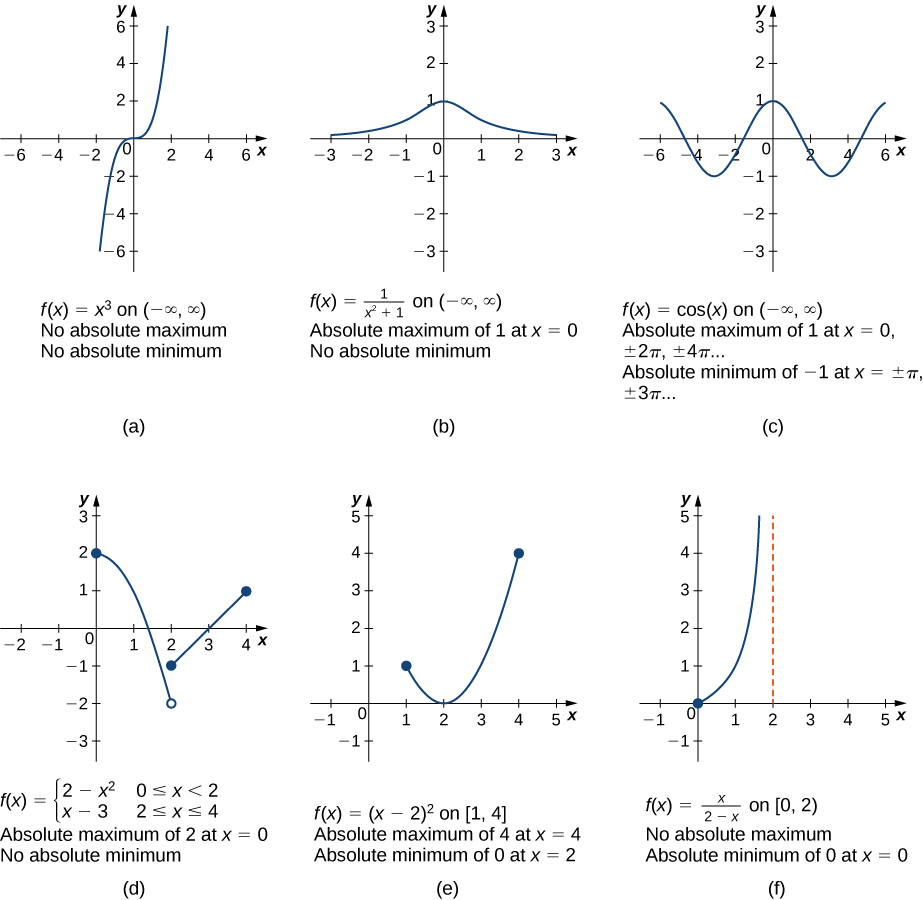
\includegraphics[width=0.8\linewidth]{img/CNX_Calc_Figure_04_03_010.jpeg}
\end{fullwidth}

\end{definition}

\begin{theorem}

\textbf{(Extreme Value Theorem):}

If \(f\) is a continuous function over the closed, bounded interval
\([a,b]\), then there is a point in \([a,b]\) at which \(f\) has an
absolute maximum over \([a,b]\) and there is a point in \([a,b]\) at
which \(f\) has an absolute minimum over \([a,b]\).

\end{theorem}

\begin{definition}

A function \(f\) has a \textbf{local maximum} at \(c\) if there exists
an open interval \(I\) containing \(c\) such that \(I\) is contained in
the domain of \(f\) and \(f(c)\ge f(x)\) for all \(x\) in \(I\). A function
\(f\) has a \textbf{local minimum} at \(c\) if there exists an open
interval \(I\) containing \(c\) such that \(I\) is contained in the
domain of \(f\) and \(f(c) \le f(x)\) for all \(x\) in \(I\). A function
\(f\) has a \textbf{local extremum} at \(c\) if \(f\) has a local
maximum at \(c\) or \(f\) has a local minimum at \(c\).

A local extremum is also known as a relative extremum.

\end{definition}

\begin{theorem}

\textbf{(Fermat's Theorem):} If \(f\) has a local extremum at \(c\) and
\(f\) is differentiable at \(c\), then \(f'(c)=0.\)

\end{theorem}

\begin{definition}

Let \(c\) be an interior point in the domain of \(f\). We say that \(c\)
is a critical point of \(f\) if \(f'(c)=0\) or \(f'(c)\) is undefined.

\begin{fullwidth}
  \centering
  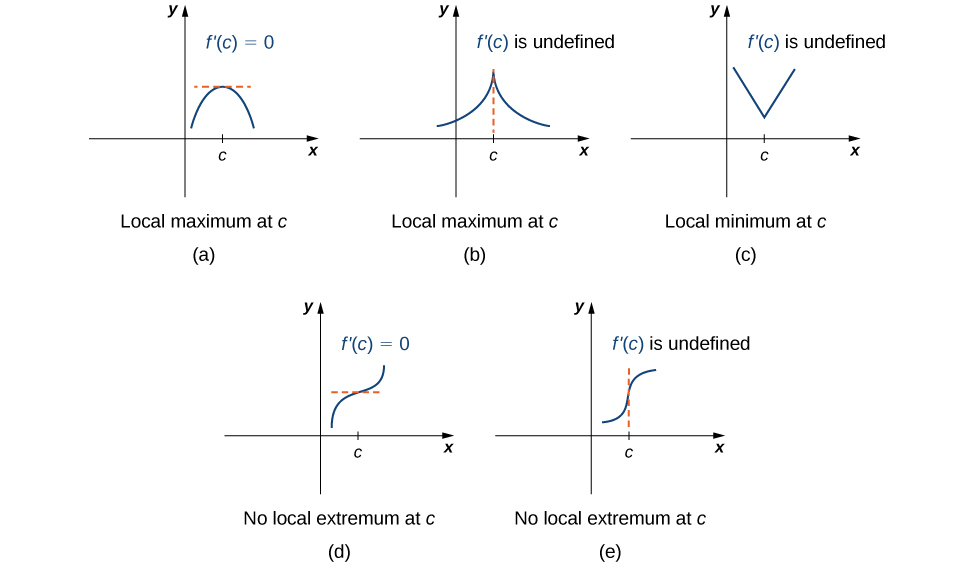
\includegraphics[width=0.8\linewidth]{img/CNX_Calc_Figure_04_03_004.jpeg}
\end{fullwidth}

\end{definition}

\begin{example}

For each of the following functions, find all critical points and
determine whether the function has a local extremum at each of the
critical points.

\begin{enumerate}
\item
  \(f(x)=\frac{1}{3}x^3 - \frac{3}{2}x^2-4x\)
\item
  \(f(x)=\frac{x}{x^2-1}\)
\end{enumerate}

\end{example}

\hypertarget{where-to-locate-absolute-extrema}{%
\subsection{Where to locate absolute
extrema}\label{where-to-locate-absolute-extrema}}

The absolute maximum of a function \(f\) over \(I\) and the absolute
minimum of \(f\) over a closed interval \(I\) must occur at endpoints of
\(I\) or at critical points of \(f\) in \(I\).

\begin{example}

For each of the following functions, find points where the function has
the absolute maximum or absolute minimum over the given interval.

\begin{enumerate}
\item
  \(f(x)= - x^2-2x - 3\) over \([0,4].\)
\item
  \(f(x)=x^2 - 3x^{2/3}\) 2. over \([0,2]\).
\end{enumerate}

\end{example}

\begin{example}

Find the absolute maximum and absolute minimum of the function
\(f(x)=\sin(x)+\cos(x)\).

\end{example}
\vspace*{6\baselineskip}

\begin{example}

Find the absolute maximum and absolute minimum of the function
\[f(x)=|x+1|+|x-1|\quad\text{over}\quad [-3,2].\]

\end{example}
\vspace*{6\baselineskip}

\begin{example}

Find the absolute maximum and absolute minimum of the function
\[f(x)=x\sqrt{4-x^2}.\]

\end{example}
\vspace*{6\baselineskip}

\subsection{Practice}

\begin{exercise}

Find the critical values of the function \[f(x)=3\sqrt{x}+x^2.\]

\end{exercise}
\vspace*{6\baselineskip}

\begin{exercise}

Find the critical values of the function \[f(x)=|x^2-2x-8|.\]

\end{exercise}
\vspace*{6\baselineskip}

\begin{exercise}

Find the absolute maximum and absolute minimum of the function
\[f(x)=4x-x^2\quad\text{over}\quad [-3,6].\]

\end{exercise}
\vspace*{6\baselineskip}

\begin{exercise}

Find the absolute maximum and absolute minimum of the function
\[g(x)=3x+6\sin x \quad\text{over}\quad [0,\pi].\]

\end{exercise}
\vspace*{6\baselineskip}

\begin{exercise}

Find the absolute maximum and absolute minimum of the function
\[h(x)=x^2\sqrt{9x-x^2}.\]

\end{exercise}



\newlecture
% !TeX root = main.tex

\hypertarget{mean-value-theorem}{%
\section{Mean Value Theorem}\label{mean-value-theorem}}

\hypertarget{rolles-theorem}{%
\subsection{Rolle's Theorem}\label{rolles-theorem}}

Let \(f\) be a function continuous over a closed interval \([a,b]\) and
differentiable over the open interval \((a,b)\). If \(f(a)=f(b)\), then
exists at least one value \(c\) in \((a,b)\) such that \(f'(c)=0\).

\begin{fullwidth}
  \centering
  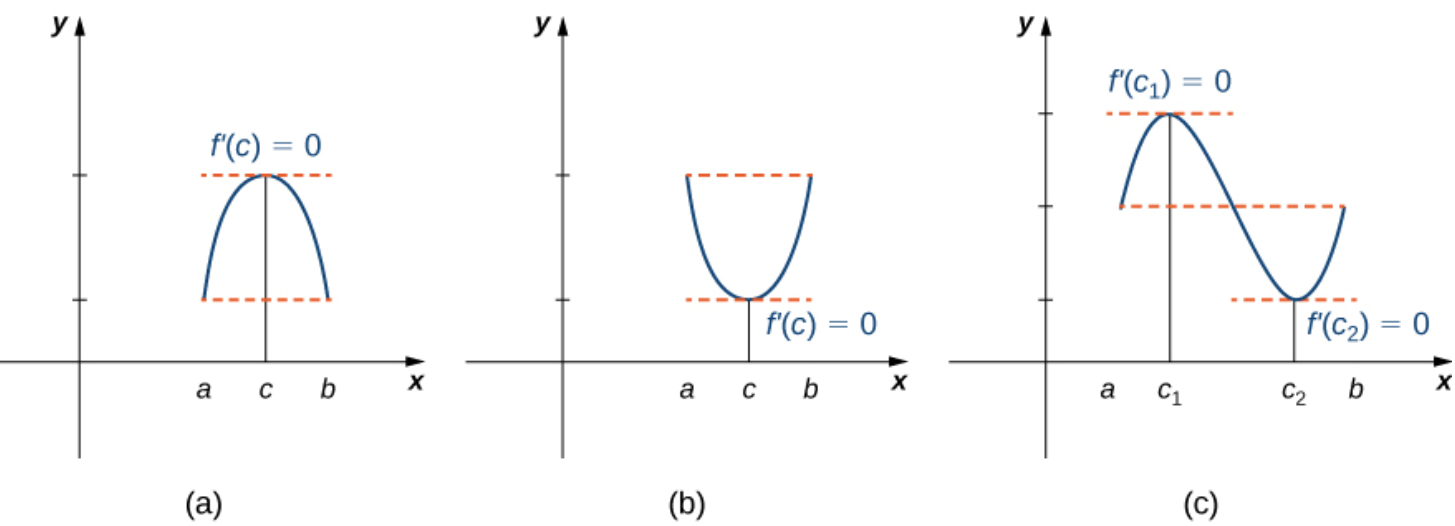
\includegraphics[scale=0.3]{img/image-20200323191523596.png}
\end{fullwidth}

\textbf{Warning:} Differentiability is important. The following is a
counter-example.

  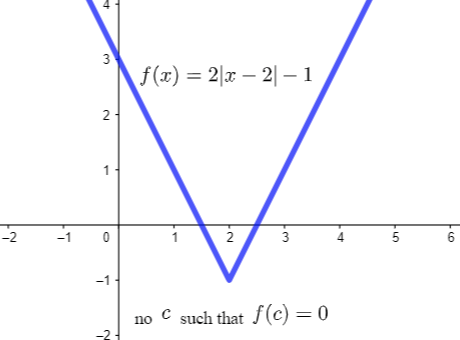
\includegraphics[scale=0.4]{img/image-20200323191152101.png}

\begin{example}

Verify that the function \(f(x)=x^2+4x-3\) satisfies the criteria stated
in Rolle's theorem and find all values \(c\) in the interval \((-3, 3)\)
at where \(f'(c)=0\).

\end{example}
\vspace*{6\baselineskip}

\begin{example}

Verify that the function \(f(x)=\sin x\) satisfies the criteria stated
in Rolle's theorem and find all values \(c\) in the interval
\((-\pi, \pi)\) at where \(f'(c)=0\).

\end{example}
\vspace*{6\baselineskip}

\hypertarget{mean-value-theorem-1}{%
\subsection{Mean Value Theorem}\label{mean-value-theorem-1}}

\begin{theorem}

Let \(f\) be a function continuous over a closed interval \([a,b]\) and
differentiable over the open interval \((a,b)\). Then exists at least
one value \(c\) in \((a,b)\) such that \[f'(c)=\frac{f(b)-f(a)}{b-a}.\]
\begin{fullwidth}
  \centering
  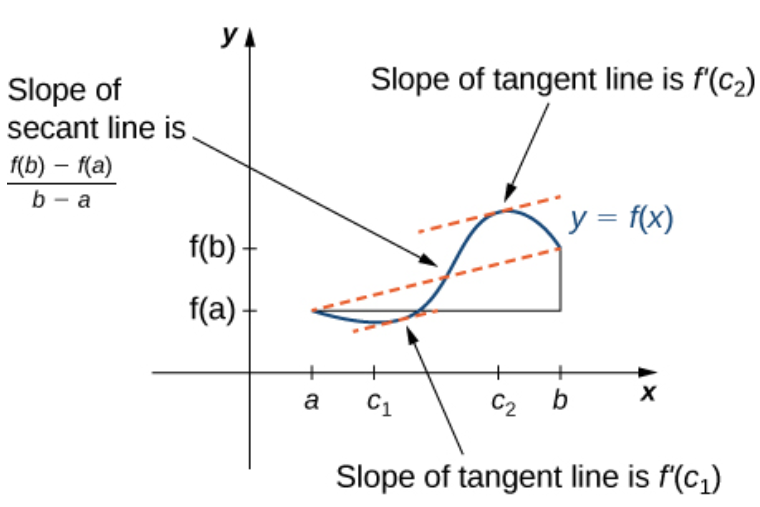
\includegraphics[scale=0.4]{img/image-20200323192552917.png}
\end{fullwidth}

\end{theorem}

To prove the theorem, let
\(g(x)=f(x) - [\frac{f(b) - f(a)}{b - a}(x - a)+f(a)]\), then apply Rolle's
theorem.

\begin{example}

Verify the function \(f(x)=\sqrt{x}\) defined over the interval
\([0,9]\) satisfies the condition of the Mean Value Theorem, and show
that there exists a value \(c\) in \((0,4)\) such that \(f'(c)\) is
equal to the slope of the secant line passing through \((0,f(0))\) and
\((9,f(9))\). Find these values \(c\) guaranteed by the Mean Value
Theorem.

\end{example}
\vspace*{6\baselineskip}

\begin{example}

Suppose that \(f(0)=-1\) and \(f'(x)>2\) for all values of \(x\) in
\([-2, 5]\). How large can \(f(x)\) possibly be?

\end{example}
\vspace*{6\baselineskip}

\hypertarget{corollaries-of-the-mean-value-theorem}{%
\subsection{Corollaries of the Mean Value
Theorem}\label{corollaries-of-the-mean-value-theorem}}

\begin{corollary}

Let \(f\) be a function differentiable over an interval \((a, b)\). If
\(f'(x)=0\) for all \(x\) in \((a, b)\), then \(f(x)=c\) for all \(x\)
in \((a, b)\), where \(c\) is a constant.

\end{corollary}

\begin{corollary}

Let \(f\) and \(g\) be two functions differentiable over an interval
\((a, b)\). If \(f'(x)=g'(x)\) for all \(x\) in \((a, b)\), then
\(f(x)=g(x)+c\) for all \(x\) in \((a, b)\), where \(c\) is a constant.

\end{corollary}

\begin{corollary}

Let \(f\) be a function continuous over the closed interval \([a,b]\)
and differentiable over the open interval \((a,b)\).

\begin{itemize}
\item
  If \(f'(x)>0\) for all \(x\) in \((a, b)\), then \(f\) is increasing
  over \((a, b)\).
\item
  If \(f'(x)<0\) for all \(x\) in \((a, b)\), then \(f\) is decreasing
  over \((a, b)\).
\end{itemize}

\end{corollary}

\begin{example}

Show that the equation \(2x-\sin x=0\) has exactly one real root.

\end{example}
\vspace*{6\baselineskip}

\subsection{Practice}

\begin{exercise}

Verify that the function \(f(x)=\cos^2x\) satisfies the criteria stated
in Rolle's theorem and find all values \(c\) in the interval
\((-\pi, \pi)\) at where \(f'(c)=0\).

\end{exercise}
\vspace*{6\baselineskip}

\begin{exercise}

Suppose that \(f(-1)=2\) and \(f'(x)<3\) for all values of \(x\) less
that 6. How small can \(f(x)\) possibly be?

\end{exercise}
\vspace*{6\baselineskip}

\begin{exercise}

Show that the equation \(x^2-2+\cos x=0\) has exactly one real root.

\end{exercise}



\newlecture
% !TeX root = main.tex

\hypertarget{monotonicity-and-concavity}{%
\section{Monotonicity and Concavity}\label{monotonicity-and-concavity}}

\hypertarget{monotonicity-test}{%
\subsection{Monotonicity Test}\label{monotonicity-test}}

\begin{proposition}

\textbf{(Increasing/Decreasing Test)} Let \(f\) be a function
differentiable on an interval \(I\).

\begin{enumerate}[sepno]
\item
  If \(f'(x)>0\) on an interval \(I\), then f is increasing on that
  interval \(I\).
\item
  If \(f'(x)<0\) on an interval \(I\), then f is decreasing on that
  interval \(I\).
\end{enumerate}

\end{proposition}

\begin{example}

Show that \(f(x)=x^2-2x\) is decreasing on \((-\infty, 1)\) and
increasing on \((1,\infty)\).

\end{example}
\vspace*{6\baselineskip}

\begin{example}

Find intervals where \(f(x)=x-2\cos x\) is increasing or decreasing.

\end{example}
\vspace*{6\baselineskip}

\begin{proposition}

\textbf{(First Derivative Test for a Local Extremum)} Let \(f\) be a
function continuous on \((a, b)\) and differentiable on
\((a, b)\setminus\{c\}\).

\begin{enumerate}[sepno]
\item
  If \(f'(x)\) chance from positive to negative when \(x\) moves to the
  right passing \(c\), then \(f\) has a local maximum at \(c\).
\item
  If \(f'(x)\) chance from negative to positive when \(x\) moves to the
  right passing \(c\), then \(f\) has a local minimum at \(c\).
\item
  If \(f'(x)\) has the same sign on both sides of \(c\), then \(f\) does
  not have a local extremum at \(c\).
\end{enumerate}

\begin{fullwidth}
  \centering
  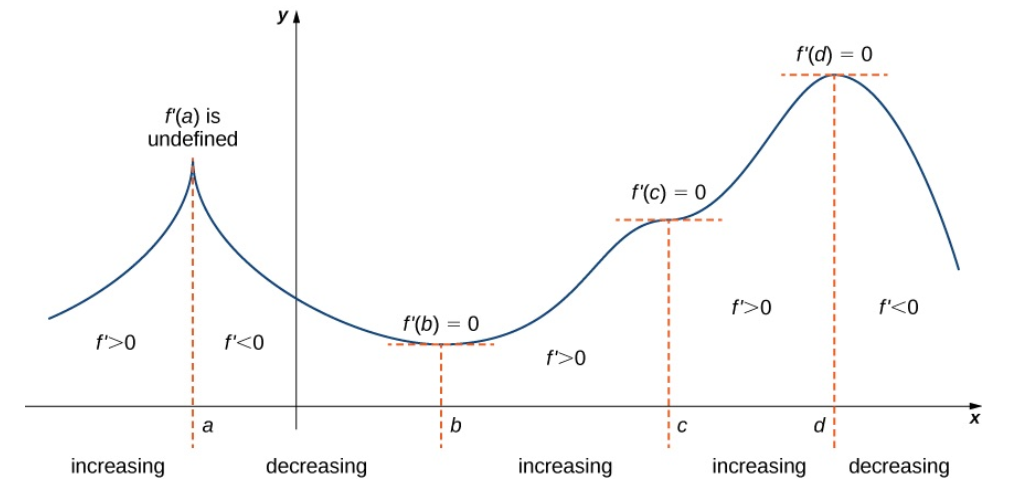
\includegraphics[scale=0.6]{img/image-20200413134520221.png}
\end{fullwidth}

\end{proposition}

\begin{example}

Use the first derivative test to find the location of all local extrema
for \(f(x)=x^3 - 3x^2 - 9x - 1\).

\end{example}
\vspace*{6\baselineskip}

\begin{example}

Use the first derivative test to find the location of all local extrema
for \(f(x)=5x^{1/3} - x^{5/3}\).

\end{example}
\vspace*{6\baselineskip}

\hypertarget{concavity-test}{%
\subsection{Concavity Test}\label{concavity-test}}

\begin{definition}

If the graph of \(f\) lies above all of its tangents on an interval
\(I\), then it is called \textbf{\emph{concave upward}} on \(I\). If the
graph of \(f\) lies below all of its tangents on \(I\), it is called
\textbf{\emph{concave downward}} on \(I\).

\begin{fullwidth}
  \centering
  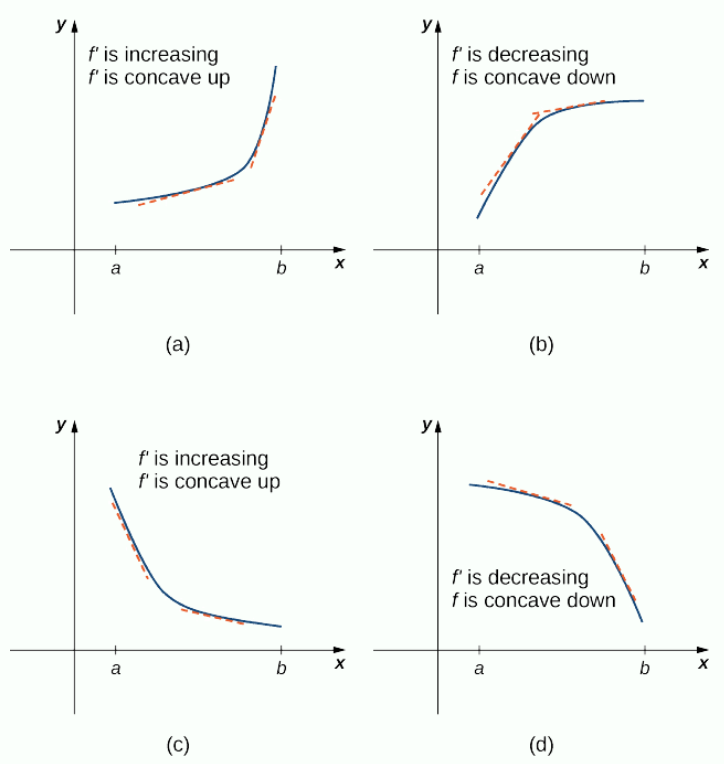
\includegraphics[scale=0.6]{img/image-20200413135215226.png}
\end{fullwidth}

A point \(P\) on a curve \(y=f(x)\) is called an
\textbf{\emph{inflection point}} if \(f\) is continuous at \(P\) and the
curve changes the direction of concavity at \(P\).

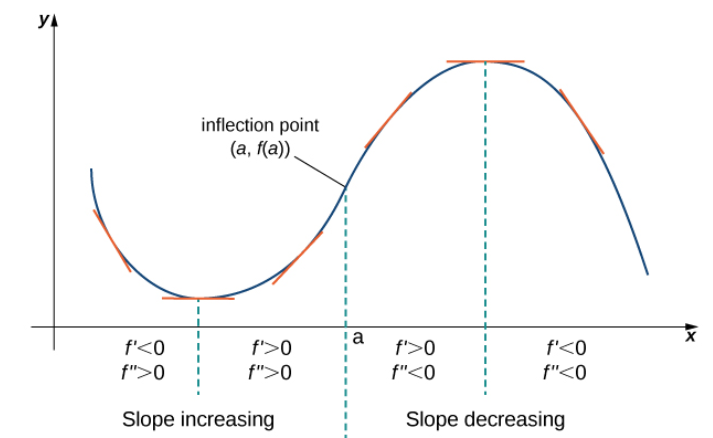
\includegraphics[scale=0.4]{img/image-20200413135252785.png}

\end{definition}

\begin{proposition}

\textbf{(Concavity Test)} Let \(f\) be a function on \((a, b)\).

\begin{enumerate}
\item
  If \(f''(x)>0\) on \((a, b)\), then \(f\) is concave upward on
  \((a, b)\).
\item
  If \(f''(x)<0\) on \((a, b)\), then \(f\) is concave downward on
  \((a, b)\).
\end{enumerate}

\end{proposition}

\begin{example}

For the function \(f(x)=x^3 - 6x^2+9x+30\), determine all intervals where
\(f\) is concave up and all intervals where \(f\) is concave down. List
all inflection points for \(f\).

\end{example}
\vspace*{6\baselineskip}

\begin{proposition}

\textbf{(Second Derivative Test)} Let \(f\) be a function defined on
\((a, b)\). Assume that there is a number \(c\) in \((a, b)\) such that
\(f'(c)=0\) and \(f''(c)\) exists.

\begin{enumerate}
\item
  If \(f''(c)<0\), then \(f\) has local maximum value at \(c\).
\item
  If \(f''(c)>0\), then \(f\) has local minimum value at \(c\).
\end{enumerate}

\end{proposition}

\begin{example}

Consider the function \(f(x)=x^3 - \frac{3x^2}{2} - 18x\). Use the second
derivative test to determine local extrema of \(f\).

\end{example}
\vspace*{6\baselineskip}

\begin{example}

Let \(f(x)=x^3-6x^2\).

\begin{enumerate}
\item
  Find the intervals where \(f\) is increasing and where it is
  decreasing.
\item
  Find the local extrema if they exists.
\item
  Find the interval where \(f\) is concave upward and where it is
  concave downward.
\item
  Find the inflection points if they exits.
\end{enumerate}

\end{example}

\subsection{Practice}

\begin{exercise}

Determine intervals where \(f(x)=\sin x+\sin^3x\), where \(0<x<\pi\), is
increasing or decreasing.

\end{exercise}
\vspace*{6\baselineskip}

\begin{exercise}

Use the first derivative test to find the location of all local extrema
for \(f(x)=x+x^2 - x^3\).

\end{exercise}
\vspace*{6\baselineskip}

\begin{exercise}

For the function \(f(x)=x+\sin(2x)\) over
\([\frac{\pi}{2},\frac{\pi}{2}]\),

\begin{enumerate}
\item
  determine all intervals where \(f\) is concave up or concave down;
\item
  list all inflection points for \(f\).
\end{enumerate}

\end{exercise}

\begin{exercise}

Consider the function \(f(x)=\sin(\pi x)-\cos(\pi x)\) over
\(x=[-1,1]\). Determine

\begin{enumerate}
\item
  intervals where \(f\) is increasing or decreasing,
\item
  local minima and maxima of \(f\),
\item
  intervals where \(f\) is concave up and concave down, and
\item
  the inflection points of \(f\).
\end{enumerate}

\end{exercise}

\begin{exercise}

Consider the function \(f(x)=\frac{1}{1 - x}\), where \(x\neq 1\).
Determine

\begin{enumerate}
\item
  intervals where \(f\) is increasing or decreasing,
\item
  local minima and maxima of \(f\),
\item
  intervals where \(f\) is concave up and concave down, and
\item
  the inflection points of \(f\).
\end{enumerate}

\end{exercise}



\newlecture
% !TeX root = main.tex

\hypertarget{curve-sketching}{%
\section{Curve Sketching}\label{curve-sketching}}

\hypertarget{limits-at-infinity}{%
\subsection{Limits at Infinity}\label{limits-at-infinity}}

\begin{definition}

Let \(f\) be a function defined on an interval \((a, \infty)\). If the
values of \(f(x)\) becomes arbitrarily close to \(L\) as \(x\) becomes
sufficiently large, we say the function \(f\) has a \textbf{limit at
infinity} and write \(\lim\limits_{x\to \infty}f(x)=L.\)

Let \(f\) be a function defined on an interval \((-\infty, a)\). If the
value of \(f(x)\) becomes arbitrarily close to \(L\) for as \(-x\)
becomes sufficiently large, we say that the function \(f\) has a
\textbf{limit at negative infinity} and write
\(\lim\limits_{x\to -\infty}f(x)=L.\)

\end{definition}


\begin{remark}

For limits at infinity, limit laws still work.

\end{remark}

\begin{example}

Consider the function \(f(x)=2+\frac1x\). Find
\(\lim\limits_{x\to -\infty}f(x)\) and
\(\lim\limits_{x\to \infty}f(x)\).

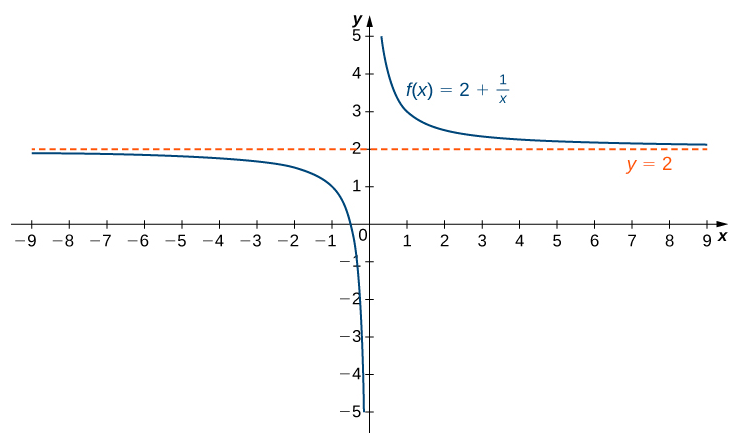
\includegraphics[width=0.9\textwidth]{img/image-20200415101551680.png}

\end{example}
\vspace*{2\baselineskip}

\begin{theorem}

Let \(p(x)=a_nx^n+a_{n-1}x^{n-1}+\cdots + a_{1}x+a_0\) and
\(q(x)=b_m x^m+b_{m-1}x^{m-1}+\cdots + b_1x+b_0\) are two polynomials.
Then \[
\lim\limits_{x\to \pm\infty}\frac{p(x)}{q(x)}=
\begin{cases}
0 & \text{if}~ n<m\\
\frac{a_n}{b_m} & \text{if}~ n=m\\
\end{cases}
\] When \(n>m\), the limit at infinity is an infinite limit.

\end{theorem}

\textbf{Recall:} A function \(f\) has an infinite limit at \(a\) if
\(\lim\limits_{x\to a}f(x)=\infty ~\text{or}~-\infty\), where \(a\) can
be a finite number, infinity or negative infinity.

\begin{example}

Find the limits
\(\lim\limits_{x\to \infty} \frac{x^4 - 4x^3+1}{2 - 2x^2 - 7x^4}\).

\end{example}
\vspace*{6\baselineskip}

\begin{example}

Find the limit
\(\lim\limits_{x\to -\infty} =\frac{x^2+\cos(x^3)}{2 - 2x^3}\).

\end{example}
\vspace*{6\baselineskip}

\hypertarget{asymptotes}{%
\subsection{Asymptotes}\label{asymptotes}}

\begin{definition}

Let \(f\) be a function defined for \(x\) or \(-x\) sufficiently large.
If \(\lim\limits_{x\to \infty}f(x)=L\) or
\(\lim\limits_{x\to -\infty}f(x)=L\), we say the line \(y=L\) is a
\emph{horizontal asymptote} of \(f\).

Let \(f\) be a function defined near \(x=a\). If
\(\lim\limits_{x\to a^-}f(x)=\infty~\text{or}~-\infty\) or
\(\lim\limits_{x\to a^+}f(x)=\infty ~\text{or}~-\infty\), we say the
line \(x=a\) is a \emph{vertical asymptote} of \(f\).

\end{definition}

\begin{example}

Consider the function \(f(x)=1-\frac1{x-1}\). Find all horizontal and
vertical asymptotes.

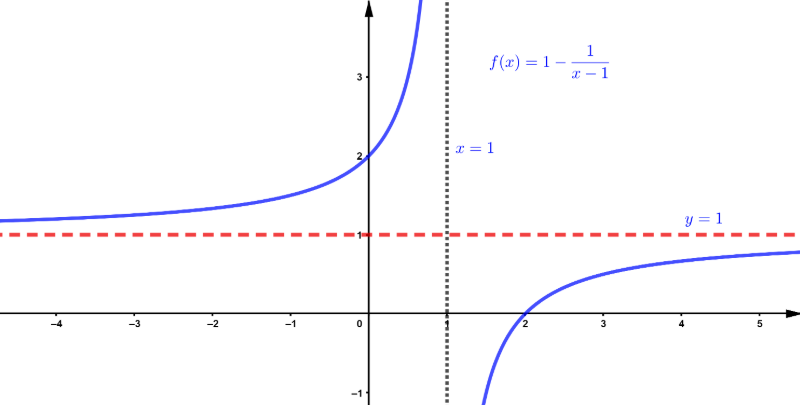
\includegraphics[width=0.9\textwidth]{img/image-20200415104515572.png}

\end{example}
\vspace*{6\baselineskip}

\begin{example}

Determine the horizontal asymptote(s) and the vertical asymptote(s) for
the function \(f\) if they exist.

\begin{enumerate}
\item
  \(f(x)=3-\frac{5}{x^2}\)
\item
  \(f(x)=\frac{\sin x}{x}\)
\end{enumerate}

\end{example}

\hypertarget{slant-asymptote}{%
\subsection{Slant Asymptote}\label{slant-asymptote}}

\begin{definition}

A line \(y=mx+b\) is a \textbf{slant asymptote} of a function \(f\) if

\[\lim\limits_{x\to \infty}[f(x)-(mx+b)]=0  ~ \text{or} ~ \lim\limits_{x\to \infty}[f(x)-(mx+b)]=0.\]

\end{definition}


\begin{example}

Determine if the function \(f(x)=\frac{x^2-2}{2x+4}\) has a slant
asymptote. If so, find it.

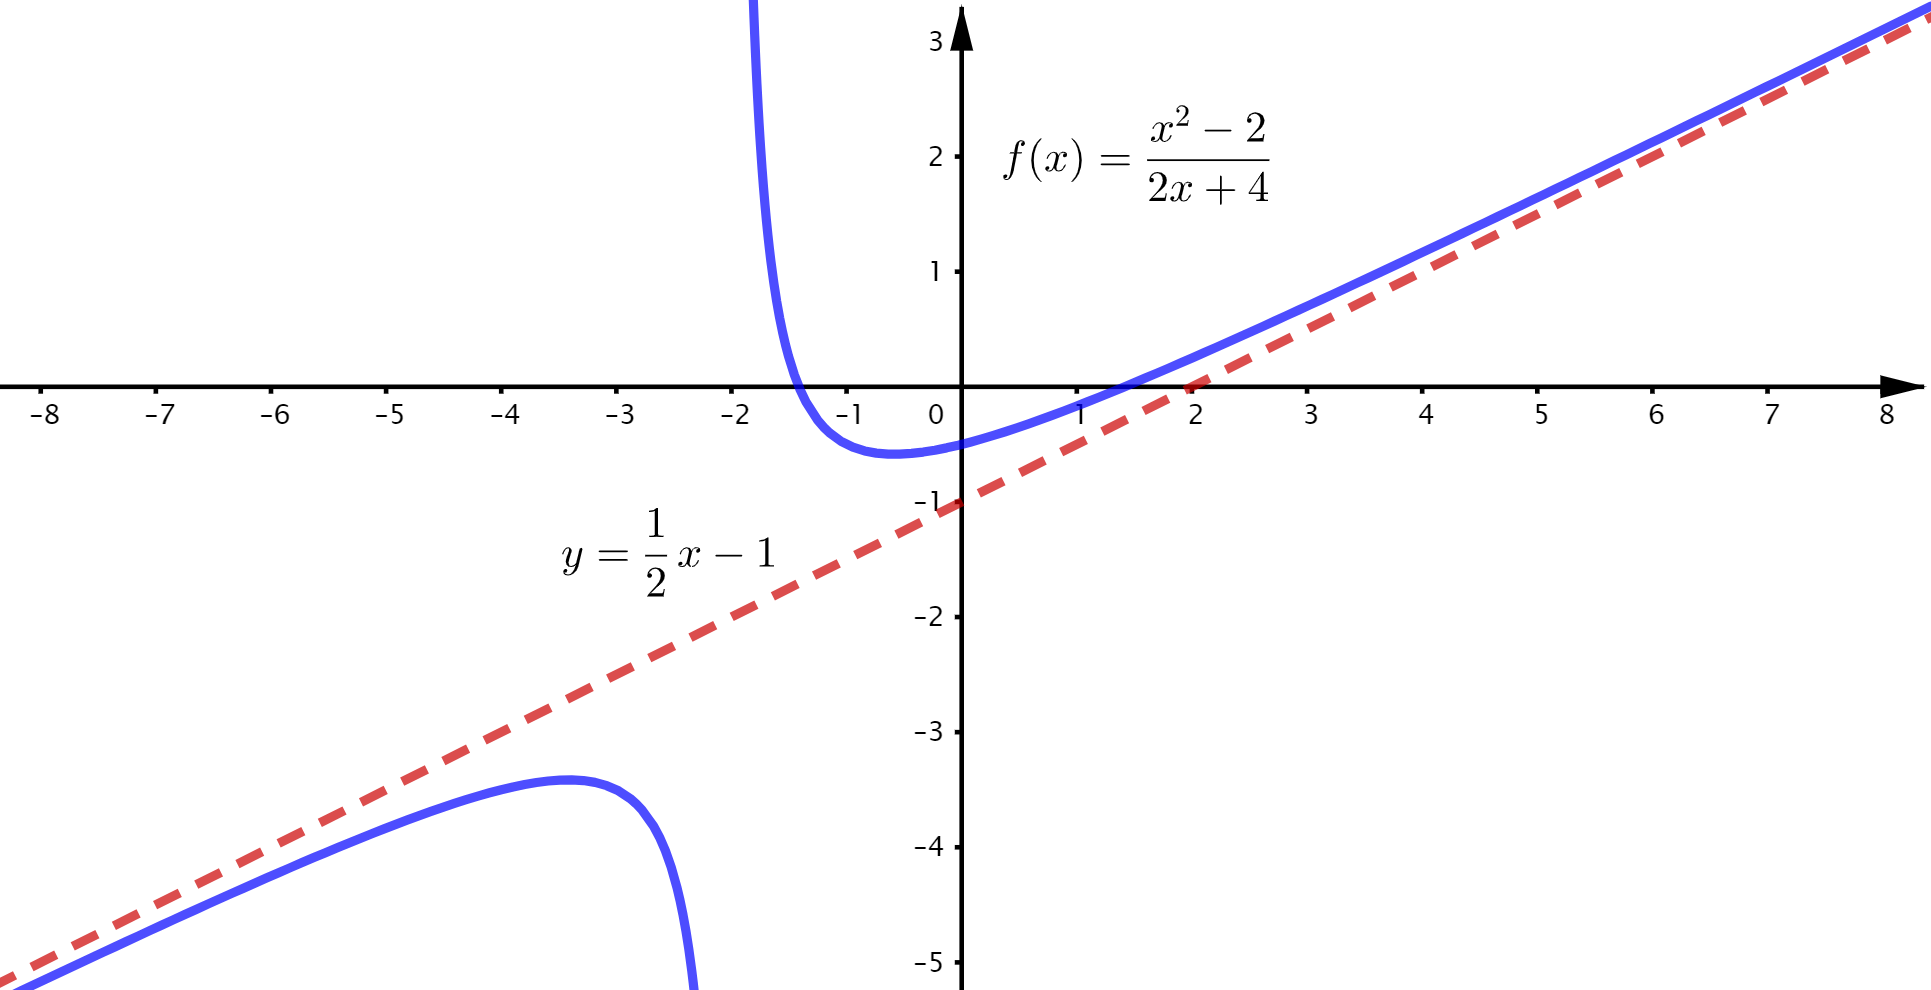
\includegraphics[width=0.9\textwidth]{img/Slant-Asymptote.png}

\end{example}
\vspace*{6\baselineskip}

\hypertarget{a-guideline-to-curve-sketching}{%
\subsection{A guideline to curve
sketching}\label{a-guideline-to-curve-sketching}}

\begin{enumerate}[sepno]
\item
  Find the domain of \(f\).
\item
  Solve for \(x\) from \(f(x)=0\) to find the \(x\)-intercepts and find
  the \(y\)-intercept \((0, f(0))\).
\item
  Determine if the function has any symmetry:

  \begin{enumerate}
  \def\labelenumii{(\alph{enumii})}
  \item
    Is \(f\) an even function, i.e.~\(f(-x)=f(x)\) for all \(x\)?
  \item
    Is \(f\) an odd function, i.e.~\(f(-x)=-f(x)\) for all \(x\)?
  \item
    Is \(f\) a periodic function, i.e.~there is a constant \(p\) such
    that \(f(x+p)=f(x)\) for all \(x\)?
  \end{enumerate}
\item
  Evaluate \(\lim\limits_{x\to -\infty} f(x)\) and
  \(\lim\limits_{x\to \infty} f(x)\) to determine the end behavior of
  \(f\). Find horizontal asymptotes if they exist.
\item
  Find vertical asymptotes if they exist.
\item
  Find slant asymptotes, i.e.~\(y=mx+b\) such that
  \(\lim\limits_{x\to \pm\infty}(f(x)-(mx+b))=0\). Note that
  \(m=\lim\limits_{x\to \infty}\frac{f(x)}{x}\) and
  \(b=\lim\limits_{x\to \infty}(f(x)-mx)\).
\item
  Calculate \(f'\) and find all critical values if they exist. Determine
  the intervals of increasing and decreasing.
\item
  Determine local extrema if they exist.
\item
  Calculate \(f''\). Determine the intervals of concave up and concave
  down. Determine inflection points if they exist.
\item
  Sketch the curve using the above information.
\end{enumerate}

\begin{example}
  
Sketch a graph of \(f(x)=(x - 1)^2(x+1).\)

\end{example}
\vspace*{10\baselineskip}


\begin{example}
  
Sketch the graph of \(f(x)=\frac{x+2}{x^2+5x+4}\).

\end{example}
\vspace*{10\baselineskip}

\subsection{Practice}

\begin{exercise}

Find the limits \(\lim\limits_{x\to -\infty}\frac{x}{x - 2}\).

\end{exercise}
\vspace*{6\baselineskip}

\begin{exercise}

Find the limit \(\lim\limits_{x\to -\infty}\frac{\sqrt{4x^2 - 1}}{x+2}\).

\end{exercise}
\vspace*{6\baselineskip}

\begin{exercise}

Find the limit
\(\lim\limits_{x\to \infty}\frac{\sqrt{x^5+1}}{x^2 - \sqrt{x}+1}\).

\end{exercise}
\vspace*{6\baselineskip}

\begin{exercise}

Determine the horizontal asymptote(s) and the vertical asymptote(s) for
the function \(f\) if they exist.

\begin{enumerate}
\item
  \(f(x)=\frac{x}{1 - x^2}\)
\item
  \(f(x)=\frac{x\sin x}{x^2 - 1}\)
\end{enumerate}

\end{exercise}

\begin{exercise}

Determine if the function \(f(x)=\frac{x^2+7x+6}{x+2}\) has a slant
asymptote. If so, find it.

\end{exercise}
\vspace*{6\baselineskip}

\begin{exercise}

Sketch the graph of \(f(x)=x^3 - 3x^2+4\).

\end{exercise}
\vspace*{10\baselineskip}

\begin{exercise}

Sketch the graph of \(f(x)=\frac{2x+3}{x^{2}+8x+12}\).

\end{exercise}
\vspace*{10\baselineskip}

\begin{exercise}

Sketch the graph of \(f(x)=\sqrt{x^2 - 5x+4}\).

\end{exercise}



\newlecture
% !TeX root = main.tex

\hypertarget{optimization-problems}{%
\section{Optimization Problems}\label{optimization-problems}}

\hypertarget{optimization-problem-solving-strategy}{%
\subsection{Optimization Problem Solving
Strategy}\label{optimization-problem-solving-strategy}}

\begin{enumerate}
\item
  Understand the Problem and represent known and unknown quantities
  using variables and expressions. In this step, it is useful to draw a
  diagram and identify variables and expressions on the diagram.
\item
  Write equations relating the variables.
\item
  Determine which quantity is to be maximized or minimized. Find the
  range of values of the other variables if possible.
\item
  Express the quantity to be maximized or minimized as an explicitly
  define function of other variables.
\item
  Locate the maximum or minimum value of the function.
\end{enumerate}

\begin{example}

A rectangular garden is to be constructed using a rock wall as one side
of the garden and wire fencing for the other three sides. Given \(100\)
ft of wire fencing, determine the dimensions that would create a garden
of maximum area. What is the maximum area?

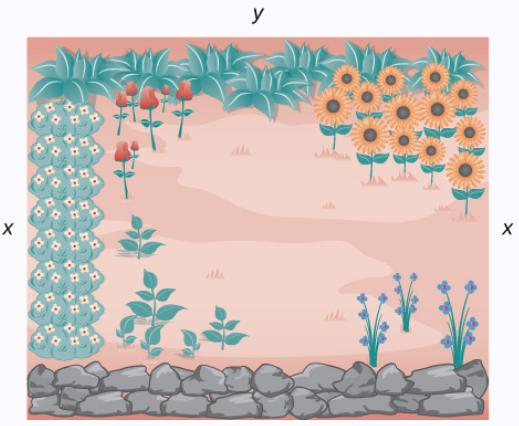
\includegraphics[width=0.9\textwidth]{img/image-20200420233408884.png}

\end{example}
\vspace*{6\baselineskip}

\begin{example}

An open-top box is to be made from a \(24\) in. by \(36\) in. piece of
cardboard by removing a square from each corner of the box and folding
up the flaps on each side. What size square should be cut out of each
corner to get a box with the maximum volume?

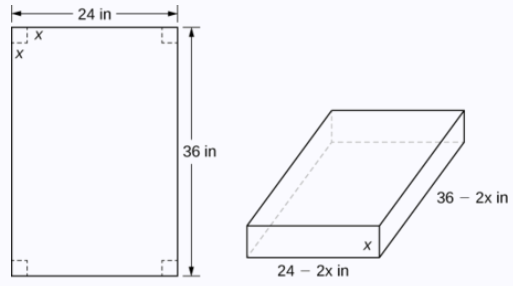
\includegraphics[width=0.9\textwidth]{img/image-20200420233831196.png}

\end{example}
\vspace*{6\baselineskip}

\begin{example}

An island is \(2\,mi\) due north of its closest point along a straight
shoreline. A visitor is staying at a cabin on the shore that is
\(6\,mi\) west of that point. The visitor is planning to go from the
cabin to the island. Suppose the visitor runs at a rate of \(8\,mph\)
and swims at a rate of \(3\,mph\). How far should the visitor run before
swimming to minimize the time it takes to reach the island?

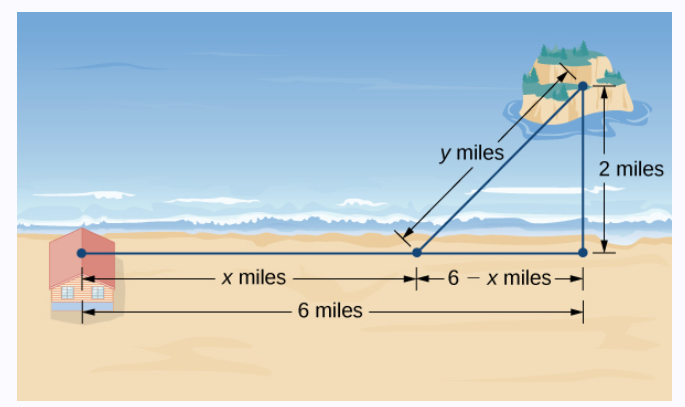
\includegraphics[width=0.9\textwidth]{img/image-20200420234008040.png}

\end{example}
\vspace*{6\baselineskip}

\begin{example}

Owners of a car rental company have determined that if they charge
customers \(p\) dollars per day to rent a car, where \(50 \le p \le 200\), the
number of cars \(n\) they rent per day can be modeled by the linear
function \(n(p)=1000 - 5p\). If they charge \(\$50\) per day or less, they
will rent all their cars. If they charge \(\$200\) per day or more, they
will not rent any cars. Assuming the owners plan to charge customers
between \(\$50\) per day and \(200\) per day to rent a car, how much
should they charge to maximize their revenue?

\end{example}
\vspace*{6\baselineskip}

\begin{example}

A rectangle is to be inscribed in the ellipse \[\dfrac{x^2}{4}+y^2=1\]
What should the dimensions of the rectangle be to maximize its area?
What is the maximum area?

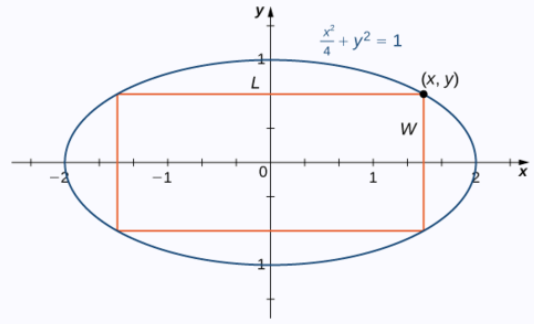
\includegraphics[width=0.9\textwidth]{img/image-20200420234107555.png}

\end{example}
\vspace*{6\baselineskip}

\hypertarget{first-derivative-test-for-absolute-extreme-values}{%
\subsection{First Derivative Test for Absolute Extreme
Values}\label{first-derivative-test-for-absolute-extreme-values}}

\begin{theorem}

Suppose that \(c\) is a critical number of a continuous function \(f\)
defined on an interval.

\begin{enumerate}
\item
  If \(f^{\prime}(x)>0\) for all \(x<c\) and \(f^{\prime}(x)<0\) for all
  \(x>c,\) then \(f(c)\) is the absolute maximum value of \(f\).
\item
  If \(f^{\prime}(x)<0\) for all \(x<c\) and \(f^{\prime}(x)>0\) for all
  \(x>c,\) then \(f(c)\) is the absolute minimum value of \(f\).
\end{enumerate}

\end{theorem}

\begin{example}

A closed box with a square base is to contain 180 cubic feet. The bottom
costs \$4 per square foot, the top costs \$1 per square foot, and the
sides cost \$3 per square foot. Find the dimensions that will minimize
the cost.

\end{example}
\vspace*{6\baselineskip}

\begin{example}

A cylindrical can is to be made to hold 1 L of tomato sauce. Find the
dimensions that will minimize the cost of the metal to manufacture the
can.

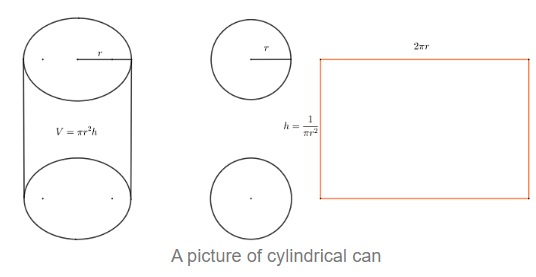
\includegraphics[width=0.9\textwidth]{img/image-20200420234447905.png}

\end{example}
\vspace*{6\baselineskip}

\subsection{Practice}

\begin{exercise}

To carry a suitcase on an airplane, the
\(\text{length} + \text{width} + \text{height}\) of the box must be less
than or equal to 62 in.

\begin{enumerate}
\item
  Assuming the height is fixed, show that the maximum volume is
  \(V=h(31 - (\frac{1}{2})h)^2.\)
\item
  What height allows you to have the largest volume?
\end{enumerate}

\end{exercise}

\begin{exercise}

Two poles are connected by a wire that is also connected to the ground.
The first pole is 20 ft tall and the second pole is 10 ft tall. There is
a distance of 30 ft between the two poles. Where should the wire be
anchored to the ground to minimize the amount of wire needed?

\end{exercise}
\vspace*{6\baselineskip}

\begin{exercise}

For every \(x\) pizzas sold, a pizzeria would make a revenue of
\(R(x)=12x\). It is known that the cost of the pizzeria to make \(x\)
pizzas is \(C(x)=2x+x^2\). How many pizzas sold would maximize the
profit?

\end{exercise}
\vspace*{6\baselineskip}

\begin{exercise}

At where is the parabola \(y=x^2\) closest to point \((0,3)\)?

\end{exercise}
\vspace*{6\baselineskip}

\begin{exercise}

A top-opened cylinder has the volume \(16\pi\). Find the dimensions of
the cylinder that has the least amount of surface area.

\end{exercise}



\newlecture
% !TeX root = main.tex

\hypertarget{antiderivatives}{%
\section{Antiderivatives}\label{antiderivatives}}

\begin{definition}

A function \(F\) is an antiderivative of the function \(f\) if
\[F'(x)=f(x)\] for all \(x\) in the domain of \(f\).

\end{definition}

\hypertarget{the-most-general-form-of-an-antiderivative}{%
\subsection{The most general form of an
antiderivative}\label{the-most-general-form-of-an-antiderivative}}

Let \(F\) be an antiderivative of \(f\) over an interval \(I\). Then, by
the mean value theorem, for each constant \(C\), the function \(F(x)+C\)
is also an antiderivative of \(f\) over \(I\); if \(G\) is an
antiderivative of \(f\) over \(I\), there is a constant \(C\) for which
\(G(x)=F(x)+C\) over \(I\). In other words, the most general form of the
antiderivative of \(f\) over \(I\) is \(F(x)+C\).

\begin{example}

For each of the following functions, find all antiderivatives.

\begin{enumerate}
\item
  \(f(x)=3x^2\)
\item
  \(f(x)=\dfrac{1}{x}\)
\item
  \(f(x)=\cos x\)
\end{enumerate}

\end{example}

\hypertarget{rules-of-antiderivatives}{%
\subsection{Rules of Antiderivatives}\label{rules-of-antiderivatives}}

\begin{longtable}[]{@{}cc@{}}
\toprule()
Function & An antiderivative \\
\midrule()
\endhead
\(af+bg\) & \(aF+bG\) \\
\(x^n\), \(n\neq -1\) & \(\frac{x^{n+1}}{n+1}\) \\
\(\sin x\) & \(-\cos x\) \\
\(\cos x\) & \(\sin x\) \\
\(\sec^2x\) & \(\tan x\) \\
\(\sec x\tan x\) & \(\sec x\) \\
\bottomrule()
\end{longtable}

In the above table, \(F\) and \(G\) are antiderivative of \(f\) and
\(g\) respectively, \(a\) and \(b\) are arbitrary constants.

\begin{example}

Find the most general antiderivative for each functions.

\begin{enumerate}
\item
  \((5x^3-7x^2+3x+4)\)
\item
  \(\dfrac{x^2+4\sqrt[3]{x}}{x}\)
\item
  \(\dfrac{4}{1+x^2}\)
\item
  \(\tan x\cos x\)
\end{enumerate}

\end{example}

\hypertarget{antiderivative-with-initial-value}{%
\subsection{Antiderivative with initial
value}\label{antiderivative-with-initial-value}}

The most general antiderivative defines a family of curves. If a point
is given, then there will be specific antiderivative. The problem of
finding a function \(y\) that satisfies a differential equation
\(\dfrac{dy}{dx}=f(x)\) with the additional condition \(y(x_0)=y_0\) is
known as an initial-value problem. The condition \$ y(x\_0)=y\_0\$ is
known as an initial condition.

\begin{example}

Solve the initial-value problem
\[\dfrac{dy}{dx}=\sin x,\quad\text{with}\quad y(0)=5.\]

\end{example}
\vspace*{6\baselineskip}

\begin{example}

Find an equation for the function \(y\) that satisfies the following
conditions \[\dfrac{dy}{dx}=3x^{-2},\quad\text{and}\quad y(1)=2.\]

\end{example}
\vspace*{6\baselineskip}

\begin{example}

Find an equation for the function \(f\) that satisfies the following
conditions \[f''(x)=\sin x,\quad f'(0)=1, \text{and}\quad f(\pi)=0.\]

\end{example}
\vspace*{6\baselineskip}

\hypertarget{application}{%
\subsection{Application}\label{application}}

\begin{example}

A car is traveling at the rate of \(88 \text{ ft}/\text{s}\) when the
brakes are applied. The car begins decelerating at a constant rate of
\(15 \text{ ft}/\text{s}^2.\)

\begin{enumerate}
\item
  How many seconds elapse before the car stops?
\item
  How far does the car travel during that time?
\end{enumerate}

\end{example}

\hypertarget{practice}{%
\subsection{Practice}\label{practice}}

\begin{exercise}

Find the antiderivative \(F(x)\) of each function \(f(x).\)

\begin{enumerate}
\item
  \(f(x)=5x^4+4x^5\)
\item
  \(f(x)=sec^2(x)+1\)
\item
  \(f(x)=2\sin x-\cos x\)
\item
  \(f(x)=\frac{x+1}{\sqrt{x}}\)
\end{enumerate}

\end{exercise}

\begin{exercise}

Solve the initial value problem.

\begin{enumerate}
\item
  \(f'(x)=x^{-3},\quad f(1)=1\)
\item
  \(f'(x)=\sqrt{x}+x^2,\quad f(0)=2\)
\item
  \(f''(x)=x^2+2,\quad f'(0)=1,\quad f(1)=2\)
\end{enumerate}

\end{exercise}

\begin{exercise}

A car is being driven at a rate of \(40\) mph when the brakes are
applied. The car decelerates at a constant rate of \(10\) ft/sec2. How
long before the car stops?

\end{exercise}



\newlecture
% !TeX root = main.tex

\hypertarget{approximating-area}{%
\section{Approximating Area}\label{approximating-area}}

\hypertarget{what-is-an-area-and-how-to-measure-it}{%
\subsection{What is an area and how to measure
it}\label{what-is-an-area-and-how-to-measure-it}}

The area of a shape can be measured by comparing the shape to squares of
a fixed size, say \(1\times1\) sized square. For a regular shape such as
a rectangle, the area can be easily measured by dividing the rectangle
into squares and taking the sum. This simple idea can be generalized to
measure irregular areas approximately. The accurate measurement of an
irregular shape needs the limit.

For areas under curve \(f\), we take the following approach.

\begin{enumerate}[sepno]
\item
  Dividing the interval \([a,b]\) into n subintervals of equal width,
  \(\Delta x=\dfrac{b - a}{n}\). Let \(x_0,x_1,x_2, \dots ,x_n\) with
  \(x_0=a,x_n=b,\) and \(x_i=x_0+i\Delta x\) be the boundary points of
  those subintervals.
\item
  The area under the curve over a subinterval \([x_{i-1}, x_i]\) can by
  estimated by \(f(x_i^*)\Delta x\), where \(x_i^*\) is a point in the
  interval \([x_{i-1}, x_i]\), and \(i=1,2,\dots, n\).
\item
  The area under the curve over \([a, b]\) is then approximately
  \[ f(x_1^*)\Delta x+f(x_2^*)+\cdots +f(x_{n-1}^*)\Delta x+f(x_n^*)\Delta x.\]
\end{enumerate}

% 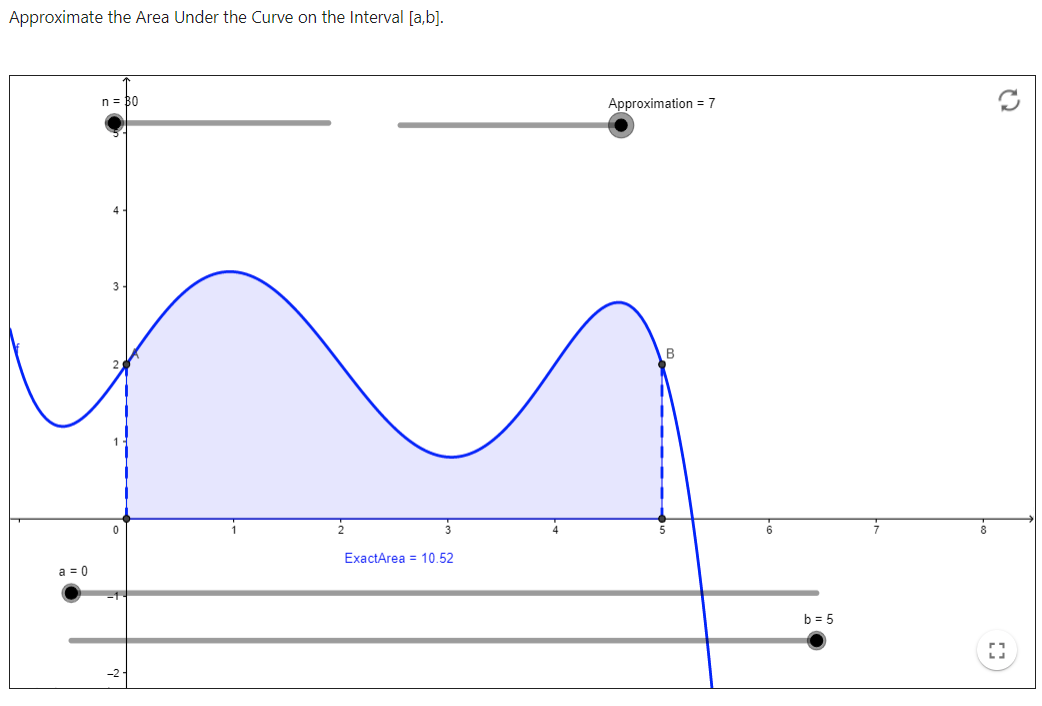
\includegraphics[width=0.9\textwidth]{img/image-20200422234011771.png}


\hypertarget{sigma-notation}{%
\subsection{Sigma Notation}\label{sigma-notation}}

For convenience, we use sigma notation \(\sum\limits_{i=1}^n s_n\) to
write sums of a sequence of \(n\) values \(s_1\),\(s_2\),\(\dots\),
\(s_n\). In the sigma notation, the letter \(i\) is called \textbf{the
index}, \(1\) is the starting value and \(n\) is the ending value in the
sequence.

For example,

\[\sum\limits_{i=1}^nf(x_i^*)\Delta x:=f(x_1^*)\Delta x+f(x_2^*)+\cdots +f(x_{n-1}^*)\Delta x+f(x_n^*)\Delta x.\]

\[\sum\limits_{n=1}^{100}n:=1+2+3+\cdots+100.\]

\hypertarget{properties-of-sigma-notation}{%
\subsection{Properties of Sigma
Notation}\label{properties-of-sigma-notation}}

Let \(a_1,a_2, \dots ,a_n\) and \(b_1,b_2, \dots ,b_n\) represent two sequences of
terms and let \(c\) be a constant. The following properties hold for all
positive integers \(n\) and for integers \(m\), with \(1 \le m \le n.\)

\begin{enumerate}[sepno]
\item
  \(\displaystyle \sum_{i=1}^n c=nc\)
\item
  \(\displaystyle \sum_{i=1}^n ca_i=c\sum_{i=1}^na_i\)
\item
  \(\displaystyle \sum_{i=1}^n(a_i+b_i)=\sum_{i=1}^na_i+\sum_{i=1}^nb_i\)
\item
  \(\displaystyle \sum_{i=1}^n(a_i - b_i)=\sum_{i=1}^na_i - \sum_{i=1}^nb_i\)
\item
  \(\displaystyle \sum_{i=1}^na_i=\sum_{i=1}^ma_i+\sum_{i=m+1}^na_i\)
\end{enumerate}

\hypertarget{sum-of-powers-of-a-sequence-of-integers}{%
\subsection{Sum of powers of a sequence of
integers}\label{sum-of-powers-of-a-sequence-of-integers}}

\[\sum_{i=1}^n i=1+2+ \cdots +n=\dfrac{n(n+1)}{2}\]

\[\sum_{i=1}^n i^2=1^2+2^2+ \cdots +n^2=\dfrac{n(n+1)(2n+1)}{6}\]

\[\sum_{i=1}^n i^3=1^3+2^3+ \cdots +n^3=\dfrac{n^2(n+1)^2}{4} \]

\begin{example}

Find the sum of the values of \(2n-1\) for \(n=1,2, \dots ,100\).

\end{example}
\vspace*{6\baselineskip}

\begin{example}

Find the sum of the values of \(n^2-n+1\) for \(n=1,2, \dots ,100\).

\end{example}
\vspace*{6\baselineskip}

\hypertarget{approximating-areas}{%
\subsection{Approximating Areas}\label{approximating-areas}}

\begin{definition}

A set of points \(P={x_i}\) for \(i=0,1,2, \dots ,n\) with
\(a=x_0<x_1<x_2< \cdots <x_n=b\), which divides the interval \([a,b]\) into
subintervals of the form
\([x_0,x_1]\),\([x_1,x_2]\),\ldots,\([x_{n - 1},x_n]\) is called a
\textbf{partition} of \([a,b]\). If the subintervals all have the same
width, the set of points forms a \textbf{regular partition} of the
interval \([a,b]\).

\end{definition}

\begin{definition}

Let \(f\) be a continuous function. The sum
\[L_n=\sum\limits_{i=1}^nf(x_{i - 1})\Delta x=f(x_0)\Delta x+f(x_1)\Delta x+\cdots+f(x_{n - 1})\Delta x,\]
where \(x_0=a\), \(\Delta=\frac{b-a}{n}\) and \(x_i=a+(i-1)\Delta x\),
is called a \textbf{left-endpoint approximation} of the area under \(f\)
over the interval \([a,b]\).

Let \(f\) be a continuous function. The sum
\[R_n=\sum\limits_{i=1}^nf(x_{i})\Delta x=f(x_1)\Delta x+f(x_1)\Delta x+\cdots+f(x_{n})\Delta x,\]
where \(x_0=a\), \(\Delta=\frac{b-a}{n}\) and \(x_i=a+(i-1)\Delta x\),
is called a \textbf{right-endpoint approximation} of the area under
\(f\) over the interval \([a,b]\).

\href{https://www.geogebra.org/m/kajgu9Yu}{Definite Integral Approximations by jeromeawhite}
% {\centering 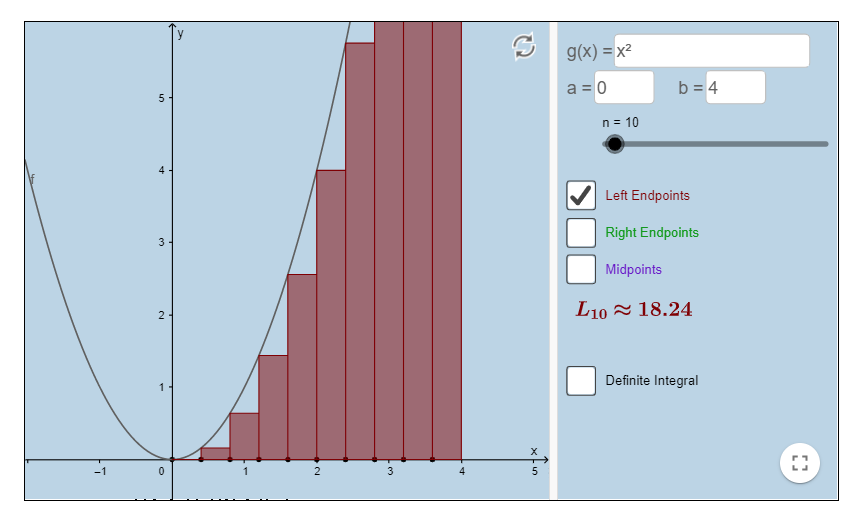
\includegraphics[scale=0.3]{img/image-20200422234746363.png}}

\end{definition}

\begin{example}

Find the left-endpoint and right-endpoint approximation of the area
under the curve \(f(x)=x^2\) over the interval \([0, 2]\) using a
partition of \(n=10\) subintervals.

\end{example}
\vspace*{6\baselineskip}

\hypertarget{riemann-sum}{%
\subsection{Riemann Sum}\label{riemann-sum}}

\begin{definition}

Let \(f(x)\) be defined on a closed interval \([a,b]\) and let \(P\) be
a regular partition of \([a,b]\). Let \(\Delta x\) be the width of each
subinterval \([x_{i - 1},x_i]\) and for each \(i\), let \(x^*_i\) be any
point in \([x_{i - 1},x_i]\). A \textbf{Riemann sum} is defined for
\(f(x)\) as \[RM_n:=\sum\limits_{i=1}^nf(x^*_i)\,\Delta x.\]

\end{definition}

\begin{definition}

A function is integrable if \(\lim\limits_{n\to \infty}R_n=A\) for any
partition of \([a, b]\).

\end{definition}

\textbf{Fact:} All functions which are continuous except at finitely
many removable or jumping discontinuities are integral.

A proof of this fact uses the \textbf{upper sum} and \textbf{lower sum}
where the sample points are where the function has max and min value
respectively. in the subinterval. Because of the continuity, the
difference between the maximum value and minimum value of \(f\) can be
make arbitrarily small by restricting to sufficiently small intervals.
That will make the difference between the upper and lower Riemann sums
neglectable.

% 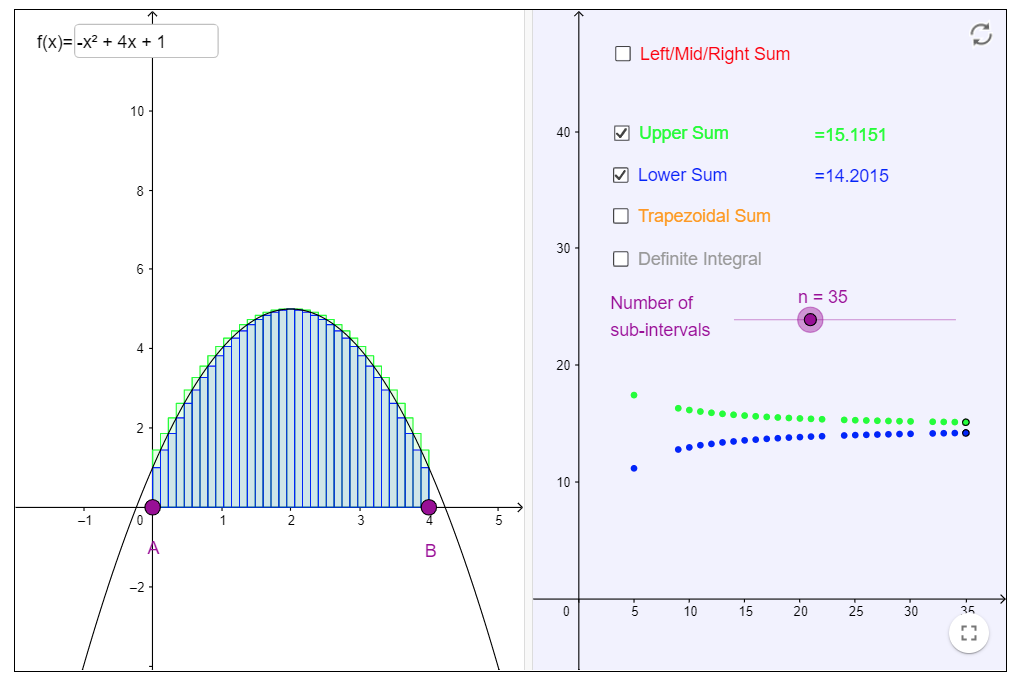
\includegraphics[width=0.9\textwidth]{img/image-20200422234550315.png}

\textbf{Fact:} For an integrable function \(f\), the area under the
curve \(f\) over \([a, b]\) is the limit of any Riemann sum. The
midpoint is also frequently used to calculate the Riemann sum.

\begin{example}

Find the lower sum and the upper sum for \(f(x)=1 - x^2\) on \([1,2]\)
using a regular partition of \(n=4\) subintervals.

\end{example}
\vspace*{6\baselineskip}

% \hypertarget{definite-integral}{%
% \subsection{Definite Integral}\label{definite-integral}}

% Let \(f(x)\) be an integrable function, particularly, a continuous
% function, defined over an interval \([a,b]\). The \textbf{definite
% integral} of \(f\) from \(a\) to \(b\) is defined as
% \[\int^b_af(x)\mathrm{d}x=\lim\limits_{n\to\infty}\sum\limits_{i=1}^nf(x^*_i)\Delta x.\]
% The numbers \(a\) and \(b\) are called the upper and lower limits of
% integration. The function \(f(x)\) is called the integrand. The
% differential \(\mathrm{d} x\) is called the variable of integration.

% Like the index in a sigma notation, the variable of integration is a
% dummy variable, which mean you may use any other letter instead of \(x\)
% to write the integral.

% \textbf{Fact:} The definite integral \(\int_a^bf(x)\mathrm{d}x\) is the
% signed area under the curve \(f\) over the interval \([a, b]\).

% \begin{example}

% Find the definite integral \(\int_0^2x\mathrm{d}x\) using a Riemann sum
% and a graph.

% \end{example}
% \vspace*{6\baselineskip}

% \begin{example}

% Find the definite integral \(\int_0^1\sqrt{1-x^2}\mathrm{d}x\) using a
% graph.

% \end{example}
% \vspace*{6\baselineskip}

\subsection{Practice}

\begin{exercise}

Find the sum of the values of \(3n+2\) for \(n=1,2, \dots ,100\).

\end{exercise}
\vspace*{6\baselineskip}

\begin{exercise}

Find the lower sum and the upper sum for \(f(x)=x^2-2x\) on \([0,2]\)
using a regular partition of \(n=5\) subintervals.

\end{exercise}
\vspace*{6\baselineskip}

% \begin{exercise}

% Find the definite integral \(\int_0^2(2x+1)\mathrm{d}x\) using a Riemann
% sum and a graph.

% \end{exercise}
% \vspace*{6\baselineskip}

% \begin{exercise}

% Find the definite integral \(\int_{-2}^0\sqrt{4-x^2}\mathrm{d}x\) using
% a graph.

% \end{exercise}



\newlecture
% !TeX root = main.tex

\hypertarget{definite-integrals}{%
\section{Definite Integrals}\label{definite-integrals}}

\hypertarget{definite-integrals-1}{%
\subsection{Definite Integrals}\label{definite-integrals-1}}

\begin{definition}

Let \(f(x)\) be an integrable function, particularly, a continuous
function, defined over an interval \([a,b]\). The \textbf{definite
integral} of \(f\) from \(a\) to \(b\) is defined as
\[\int^b_af(x)\mathrm{d}x=\lim\limits_{n\to\infty}\sum\limits_{i=1}^nf(x^*_i)\Delta x.\]
The symbol \(\int\) is called an integral sign. The numbers \(a\) and
\(b\) are called the \textbf{upper and lower limits of integration}. The
function \(f(x)\) is called the \textbf{integrand}. The
\textbf{differential} \(\mathrm{d} x\) is called the \textbf{variable of
integration}.

\end{definition}

Like the index in a sigma notation, the variable of integration is a
dummy variable, which mean you may use any other letter instead of \(x\)
to write the integral.

\textbf{Fact:} The definite integral \(\int_a^bf(x)\mathrm{d}x\) is the
signed area under the curve \(f\) over the interval \([a, b]\).

\begin{example}

Find the definite integral \(\int_a^bc\mathrm{d}x\) using a Riemann sum
and a graph.

\end{example}
\vspace*{6\baselineskip}

\begin{example}

Find the definite integral \(\int_a^bx\mathrm{d}x\) using a Riemann sum
and a graph.

\end{example}
\vspace*{6\baselineskip}

\begin{example}

Find the definite integral \(\int_{a}^bx^2\mathrm{d}x\) using a Riemann
sum.

\end{example}
\vspace*{6\baselineskip}

\begin{example}

Find the definite integral \(\int_0^1\sqrt{1-x^2}\mathrm{d}x\) using a
graph.

\end{example}
\vspace*{6\baselineskip}

\begin{example}

Express the limit as an integral and evaluate
\[\lim\limits_{x\to \infty}\frac{1}{n}\sum_{i=1}^n\frac{i^2}{n^2}\]

\end{example}
\vspace*{6\baselineskip}

\hypertarget{signed-area}{%
\subsection{Signed Area}\label{signed-area}}

\begin{definition}

\textbf{(Signed Area)} Let \(f(x)\) be an integrable function defined on
an interval \([a,b]\). Let \(A_1\) represent the area between \(f(x)\)
and the \(x\)-axis that lies above the axis and let \(A_2\) represent
the area between \(f(x)\) and the \(x\)-axis that lies below the axis.
Then, the~(net) signed area~between \(f(x)\) and the \(x\)-axis is given
by \[\int^b_af(x)\,dx=A_1 - A_2.\] The total area between \(f(x)\) and the
\(x\)-axis is given by \[\int^b_a|f(x)|\,dx=A_1+A_2.\]

\end{definition}

\begin{example}

Find the total area between the function \(f(x)=x-2\) and the \(x\)-axis
over the interval \([0,3]\).

\end{example}
\vspace*{6\baselineskip}

\hypertarget{rules-of-definite-integrals}{%
\subsection{Rules of Definite
Integrals}\label{rules-of-definite-integrals}}

\begin{enumerate}[sepno]
\item
  \[\int^a_af(x)\,\mathrm{d}x=0\] If the limits of integration are the
  same, the integral is just a line and contains no area.
\item
  \[\int^a_bf(x)\,\mathrm{d}x= - \int^b_af(x)\,\mathrm{d}x\] If the limits
  are reversed, then place a negative sign in front of the integral.
\item
  \[\int^b_a[f(x)+g(x)]\,\mathrm{d}x=\int^b_af(x)\,\mathrm{d}x+\int^b_ag(x)\,\mathrm{d}x\]
  The integral of a sum is the sum of the integrals.
\item
  \[\int^b_a[f(x) - g(x)]\,\mathrm{d}x=\int^b_af(x)\,\mathrm{d}x - \int^b_ag(x)\,\mathrm{d}x\]
  The integral of a difference is the difference of the integrals
\item
  \[\int^b_acf(x)\,\mathrm{d}x=c\int^b_af(x)\,\mathrm{d}x\] for constant
  \(c\). The integral of the product of a constant and a function is
  equal to the constant multiplied by the integral of the function.
\item
  \[\int^b_af(x)\,\mathrm{d}x=\int^c_af(x)\,\mathrm{d}x+\int^b_cf(x)\,\mathrm{d}x\]
  Although this formula normally applies when \(c\) is between \(a\) and
  \(b\), the formula holds for all values of \(a\), \(b\), and \(c\),
  provided \(f(x)\) is integrable on the largest interval.
\end{enumerate}

\begin{example}

If it is known that \(\displaystyle \int^5_1f(x)\,\mathrm{d}x= - 3\) and
\(\displaystyle \int^5_2f(x)\,\mathrm{d}x=4\), find the value of
\(\displaystyle \int^2_1f(x)\,\mathrm{d}x.\)

\end{example}
\vspace*{6\baselineskip}

\begin{theorem}

\textbf{Comparison Theorem:}

\begin{enumerate}[sepno]
\item
  If \(f(x) \ge 0\) for \(a \le x \le b\), then \[\int^b_af(x)\,\mathrm{d}x \ge 0.\]
\item
  If \(f(x) \ge g(x)\) for \(a \le x \le b\), then
  \[\int^b_af(x)\,\mathrm{d}x \ge \int^b_ag(x)\,\mathrm{d}x.\]
\item
  If \(m\) and \(M\) are constants such that \(m \le f(x) \le M\) for \(a \le x \le b\),
  then \[m(b - a) \le \int^b_af(x)\,\mathrm{d}x \le M(b - a).\]
\end{enumerate}

\end{theorem}

\begin{example}

Determine the sign of
\(\int_0^1(\sqrt{1+x^2}-\sqrt{1+x^4})\mathrm{d} x\)

\end{example}
\vspace*{6\baselineskip}

\subsection{Practice}

\begin{exercise}

Using geometry to evaluate the integral
\[\displaystyle \int^3_{ - 3}(3 - |x|)\,dx.\]

\end{exercise}
\vspace*{6\baselineskip}

\begin{exercise}

Express the limit as integrals
\[\displaystyle \lim_{n\to\infty}\sum_{i=1}^n\sin^2(2\pi x^*_i)\Delta x\quad \text{over}\quad [0,1].\]

\end{exercise}
\vspace*{6\baselineskip}

\begin{exercise}

Using integral to evaluate the limit
\[\displaystyle \lim\limits_{n\to \infty}\frac{1}{n}\sum_{i=1}^n\frac{i - 1}{n}\]

\end{exercise}
\vspace*{6\baselineskip}

\begin{exercise}

Suppose that \(\displaystyle \int^4_0f(x)\,dx=5\) and
\(\displaystyle \int^2_0f(x)\,dx= - 3\), and
\(\displaystyle \int^4_0g(x)\,dx= - 1\) and
\(\displaystyle \int^2_0g(x)\,dx=2\) Compute the following integrals.

\begin{enumerate}
\item
  \(\displaystyle \int^4_0(3f(x) - 4g(x))\,dx\)
\item
  \(\displaystyle \int^4_2(2f(x)+3g(x))\,dx\)
\end{enumerate}

\end{exercise}

\begin{exercise}

Show that
\(\displaystyle \int^{\pi/4}_{ - \pi/4}\cos t\,dt \ge \pi\sqrt{2}/4\).

\end{exercise}



\newlecture
% !TeX root = main.tex

\hypertarget{fundamental-theorem-of-calculus}{%
\section{Fundamental Theorem of
Calculus}\label{fundamental-theorem-of-calculus}}

\begin{theorem}

\textbf{(Fundamental Theorem of Calculus I)} Suppose that \(f(x)\) is
continuous on the interval \([a,b]\). If \(F(x)\) is any antiderivative
of \(f(x)\), then \[\int_a^b f(x)\,\mathrm{d}x = F(b)-F(a).\]

\end{theorem}

\begin{theorem}

\textbf{(Fundamental Theorem of Calculus II)} Suppose that \(f(x)\) is
continuous on the interval \([a,b]\) and let \[F(x)=\int_a^x f(t)\,dt.\]
Then \(F'(x)=f(x)\).

\end{theorem}

\begin{proof}[Idea of Proof] FTC I follows from FTC II by taking \(x=b\). FTC
II is following the continuity, the comparison theorem and the squeeze
theorem.
\end{proof}

\href{https://www.geogebra.org/m/wdUED3wy}{Fundamental theorem of calculus by GeoGebra Forum}

% \begin{fullwidth}
%   \centering
%   \href{https://www.geogebra.org/m/wdUED3wy}{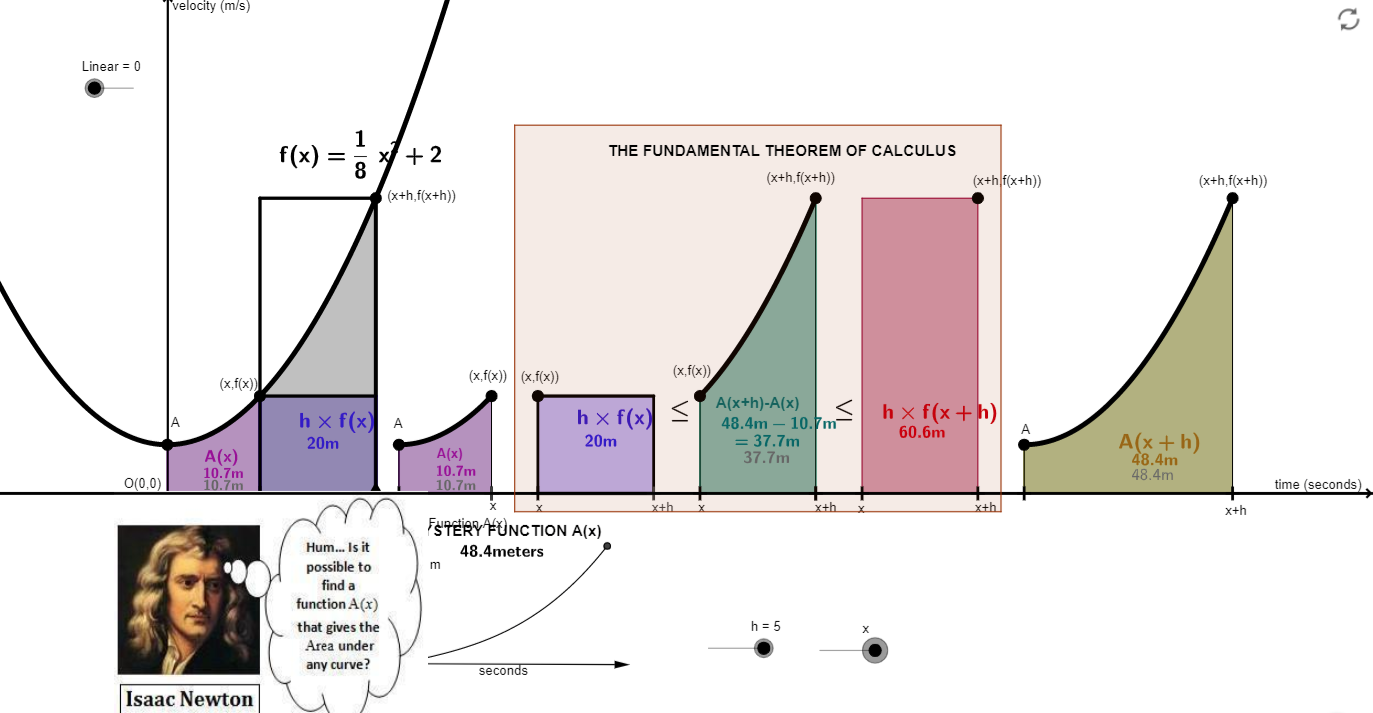
\includegraphics[width=0.8\linewidth]{img/image-20200427155419418.png}}
% \end{fullwidth}


\begin{example}

Evaluate the integral \[ \int_1^3 (x^2+3x)\,\mathrm{d}x\]

\end{example}
\vspace*{6\baselineskip}

\begin{example}

Evaluate the integral \[ \int_0^\pi \sin x \,\mathrm{d}x\]

\end{example}
\vspace*{6\baselineskip}

\begin{example}

Find the derivative of \[G(x)=\int_1^x (t^2-3t)\,dt\]

\end{example}
\vspace*{6\baselineskip}

\begin{example}

Find the derivative of \[G(x)=\int_1^{x^2} \cos(3t)\,dt\]

\end{example}
\vspace*{6\baselineskip}

\begin{example}

Find the derivative of \[G(x)=\int_x^1 \tan(t^2)\,dt\]

\end{example}
\vspace*{6\baselineskip}

\subsection{Practice}

\begin{exercise}

Evaluate the definite integral.

\begin{enumerate}
\item
  \(\displaystyle \int^2_{-1}(x^2-3x)\,dx\)
\item
  \(\displaystyle \int^3_{-2}(t+2)(t-3)dt\)
\end{enumerate}

\end{exercise}

\begin{exercise}

Find the derivative of the function.

\begin{enumerate}
\item
  \(\displaystyle f(x)=\frac{d}{dx}\int^x_3\sqrt{9-y^2}\,dy\)
\item
  \(\displaystyle f(x)=\frac{d}{dx}\int^{x^2}_0\sqrt{1-t^2}\,dt\)
\item
  \(\displaystyle f(x)=\frac{d}{dx}\int^1_{\cos x}\sqrt{1-t^2}\,dt\)
\end{enumerate}

\end{exercise}



\newlecture
% !TeX root = main.tex

\hypertarget{indefinite-integrals-and-net-changes}{%
\section{Indefinite Integrals and Net
Changes}\label{indefinite-integrals-and-net-changes}}

\begin{definition}

Let \(F\) be an antiderivative of the function \(f\), that is
\(F'(x)=f(x)\). We call the most general anti-derivative of \(f\) is the
indefinite integral and denoted as \[\int{{f(x)\,dx}} = F(x) + c,\]
where \(c\) is any constant.

\end{definition}

\textbf{Formulas of Indefinite Integrals:}

\begin{itemize}
\item
  \(\displaystyle \int\left(af( x )+bg(x)\right)\,dx = a\int f( x )\,dx + b\int g( x )\,dx\)
\item
  \(\displaystyle \int x^n \,dx = \dfrac{x^{n+1}}{n+1} + C\), as long as
  \(n \ne -1\)
\item
  \(\displaystyle \int \cos(x) \, dx = \sin(x) + C\)
\item
  \(\displaystyle \int \sin(x) \, dx = - \cos(x) + C\)
\item
  \(\displaystyle \int \sec^2(x) \, dx = \tan(x) + C\)
\item
  \(\displaystyle \int \sec(x) \tan(x) \, dx = \sec(x) + C\)
\item
  \(\displaystyle \int \csc^2(x) \, dx = - \cot(x) + C\)
\item
  \(\displaystyle \int \csc(x)\cot(x) \, dx = -\csc(x) + C\)
\end{itemize}

\begin{example}

Evaluate the following indefinite integral.

\begin{enumerate}
\item
  \(\displaystyle\int (x^4 + 3x - 2)\,dx\)
\item
  \(\displaystyle\int\sqrt{x}(x^2 - 1)\,dx\)
\item
  \(\displaystyle\int (\sin x-\sec^2 x)\,dx\)
\end{enumerate}

\end{example}

\begin{definition}

The \textbf{net change} of a quantity is the integral of the rate of
change of that quantity. \[\text{Net change}=\int_a^b r(t)\,dt\] where
\(r(t)\) is the rate of change function.

Note the \textbf{total change} is
\[\text{Total change}=\int_a^b |r(t)|\,dt\] where \(r(t)\) is the rate of
change function.

\end{definition}

\begin{example}

Water is flowing into a tank at a rate of \(r(t)=3t^2-2t\) ft\(^3\)/min.
How much water flows into the tank over the time interval 2 min. to 4
min.?

In Physics, the net and total changes are known as the displacement and
distance. The distinction is between velocity and speed.

Displacement = Net change in position = integral of velocity.

Distance traveled Total = change in position = integral of speed.

\end{example}
\vspace*{6\baselineskip}

\begin{example}

A particle moves along a straight line. The velocity is observed as a
linear function \(v(t)=2t-6\) m/s from time \(t=0\) to time \(t=3\).

\begin{enumerate}
\item
  Find the net displacement of the particle.
\item
  Find the distance the particle traveled.
\end{enumerate}

\end{example}

\begin{definition}

Suppose that \(f\) is continuous over \([a,b]\). The \textbf{average
value of the function} of \(f\) over \([a, b]\) is defined as
\[f_{ave}=\dfrac{1}{b-a}\int_a^bf(x)dx.\]

\end{definition}

\begin{example}

Let \(f\) be a continuous function over \([a, b]\). Show that there is
number \(c\) in \([a,b]\) such that
\[f(c)=\dfrac{1}{b-a}\int_a^bf(x)dx.\]

\end{example}
\vspace*{6\baselineskip}

\begin{example}

Find the average of the function \(f(x)=x^2\) over \([-2, 2]\).

\end{example}
\vspace*{6\baselineskip}

\hypertarget{integration-of-even-and-odd-functions}{%
\subsection{Integration of Even and Odd
Functions}\label{integration-of-even-and-odd-functions}}

For continuous even functions \(f\), that is \(f(-x)=f(x)\),

\[\displaystyle \int^a_{-a}f(x)\,dx=2\int^a_0f(x)\,dx.\]

For continuous odd functions \(f\), that is \(f(-x)=-f(x),\)

\[\displaystyle \int^a_{-a}f(x)\,dx=0.\]

\begin{example}

Evaluate the following integrals.

\begin{enumerate}
\item
  \(\displaystyle \int^2_{-2}(3x^4+1)\,dx\)
\item
  \(\displaystyle \int_\pi^{-\pi} 6\sin x\, dx\)
\end{enumerate}

\end{example}

\subsection{Practice}

\begin{exercise}

Evaluate the indefinite integral

\begin{enumerate}
\item
  \(\displaystyle \int (\sqrt{x}-\frac{1}{\sqrt{x}})\,dx.\)
\item
  \(\displaystyle \int(\sin x-\cos x)\,dx\)
\end{enumerate}

\end{exercise}

\begin{exercise}

Suppose that a particle moves along a straight line with velocity
\(v(t)=4-2t,\) where \(0\leq t\leq 2\) (in meters per second).

Find the displacement at time t and the total distance traveled up to
\(t=2\).

\end{exercise}
\vspace*{6\baselineskip}


\begin{exercise}

Find the average of the function
\[f(x)=\sqrt{x}\qquad\text{over}\qquad [0,4].\]

\end{exercise}
\vspace*{6\baselineskip}


\begin{exercise}

Evaluate the integral \[\int_{-2}^2 x\sqrt{x^4+1}\,dx.\]

\end{exercise}



\newlecture
% !TeX root = main.tex

\hypertarget{substitution-method}{%
\section{Substitution Method}\label{substitution-method}}

Recall rules of derivatives.

\begin{enumerate}[sepno]
\item
  Chain rule: \((f(g(x)))'=f'(g(x))g'(x)\).
\item
  Product Rule: \((f(x)g(x))'=f'(x)g(x)+f(x)g'(x)\).
\end{enumerate}

Reverse those rules, we will get techniques of integration.

\begin{theorem}

\textbf{(Substitution Method for Indefinite Integrals)} Let \(u=g(x)\),
where \(g'(x)\) is continuous over an interval, let \(f(x)\) be
continuous over the corresponding range of g, and let \(F(x)\) be an
antiderivative of \(f(x).\) Then,
\[\int f(g(x))g'(x)\mathrm{d} x =\int f(u)\,)u=F(u)+C= F(g(x))+C.\]

\end{theorem}

\begin{example}

Find the indefinite integral \[\int 2x(x^2+5)^7\mathrm{d} x.\]

\end{example}
\vspace*{6\baselineskip}

\begin{example}

Find the indefinite integral \[\int \sqrt{2x+1}\mathrm{d} x.\]

\end{example}
\vspace*{6\baselineskip}

\begin{example}

Find the indefinite integral
\[\int 8(x+1)\sqrt[3]{x^2+2x}\mathrm{d} x.\]

\end{example}
\vspace*{6\baselineskip}

\begin{example}

Find the indefinite integral
\[\int \dfrac{1}{\sqrt{x}(\sqrt{x}+1)}\mathrm{d} x.\]

\end{example}
\vspace*{6\baselineskip}

\begin{example}

Find the indefinite integral
\[\int \dfrac{\sin x}{\cos^5x}\mathrm{d} x.\]

\end{example}
\vspace*{6\baselineskip}

\begin{example}

Find the indefinite integral \[\int \cos x(2\sin x+3)^3\mathrm{d} x.\]

\end{example}
\vspace*{6\baselineskip}

\begin{example}

Find the indefinite integral
\[\int \frac{x+1}{\sqrt{x-1}}\mathrm{d} x.\]

\end{example}
\vspace*{6\baselineskip}

\begin{theorem}

\textbf{Substitution for Definite Integral}

Let \(u=g(x)\) and let \(g'\) be continuous over an interval \([a,b]\),
and let \(f\) be continuous over the range of \(u=g(x).\) Then,
\[\int^b_af(g(x))g'(x)\mathrm{d} x=\int^{g(b)}_{g(a)}f(u)\mathrm{d} u.\]

\end{theorem}

\begin{example}

Evaluate the definite integral
\[\int^1_0 x\sin\left(\dfrac{\pi x^2}{2}\right)\mathrm{d} x.\]

\end{example}
\vspace*{6\baselineskip}

\begin{example}

Evaluate the definite integral \[\int^2_1 \cos(3x-2)\mathrm{d} x.\]

\end{example}
\vspace*{6\baselineskip}

\begin{example}

Evaluate the definite integral
\[\int^1_{-2} \dfrac{x}{\sqrt{x^2+1}}\mathrm{d} x.\]

\end{example}
\vspace*{6\baselineskip}

\begin{example}

Evaluate the definite integral
\[\displaystyle \int^{3\pi/4}_{\pi/4}\sin^2 t\cos t\mathrm{d} t.\]

\end{example}
\vspace*{6\baselineskip}

\subsection{Practice}

\begin{exercise}

Evaluate the following integrals.

\begin{enumerate}
\item
  \(\displaystyle \int x\sqrt{x+1}\mathrm{d} x\)
\item
  \(\displaystyle \int\frac{x}{(4x^2+9)^2}\mathrm{d} x\)
\item
  \(\displaystyle \int(x - 2)^7\mathrm{d} x\)
\item
  \(\displaystyle \int\cos^3 \theta\sin \theta\mathrm{d} \theta\)
\end{enumerate}

\end{exercise}

\begin{exercise}

\begin{enumerate}
\item
  \(\displaystyle \int^1_0x\sqrt{1 - x^2}\mathrm{d} x\)
\item
  \(\displaystyle \int^{\pi/4}_0\sec^2 \theta \tan \theta \mathrm{d} \theta \)
\item
  \(\displaystyle \int^{\pi/4}_0\frac{\sin \theta }{\cos^4 \theta }\mathrm{d} \theta \)
\end{enumerate}

\end{exercise}



\newlecture
% !TeX root = main.tex

\hypertarget{area-between-curves}{%
\section{Area Between Curves}\label{area-between-curves}}

The idea of finding area under an curve can be generalized to finding
areas between curves. That is to slice the region enclosed by the
curves, represent the area of a slice using the functions and a
differential, and then take the sum which can be expressed as an
integral.

\begin{fullwidth}
  \centering
  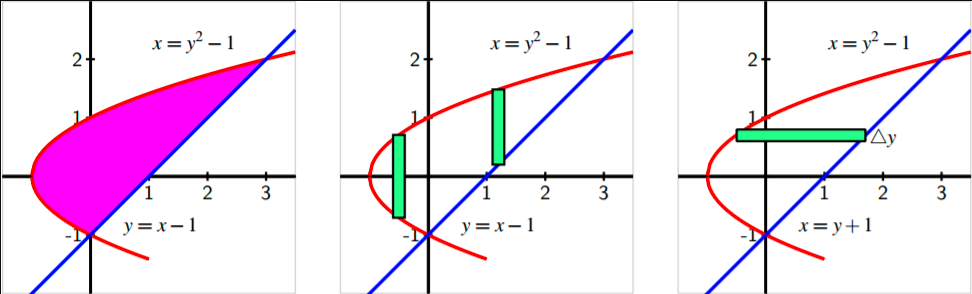
\includegraphics[width=0.8\linewidth]{img/image-20200506101055076.png}
\end{fullwidth}

\hypertarget{summarize-the-idea-we-get-the-following-strategy}{%
\subsection{Summarize the idea, we get the following
strategy}\label{summarize-the-idea-we-get-the-following-strategy}}

\begin{enumerate}[sepno]
\item
  Sketch the curves and the enclosed region.
\item
  Determine the boundaries of the region: find intersection points if
  they are on the boundary.
\item
  Draw and label the dimension of a representative slice.
\item
  State the area of the representative slice:

  \begin{itemize}
  \item
    if vertical slices are used, the area of a slice can be represented
    by \(\lvert U(x)-L(x)\rvert\, dx\), where \(U(x)\) and \(L(x)\) are
    the upper and lower curves respectively;
  \item
    if horizontal slices are used, the area of a slice can be
    represented by \(\lvert R(y)-L(y)\rvert\, dy\), where \(R(y)\) and
    \(L(y)\) are the right and left curves respectively;
  \end{itemize}
\item
  Write a definite integral to represent area:

  \begin{itemize}
  \item
    if vertical slides:
    \(\displaystyle\int^{x_R}_{x_L}\lvert U(x)-L(x)\rvert\, dx\), where
    \(x_L\) and \(x_R\) are the left and right boundaries of the region.
  \item
    if horizontal slides:
    \(\displaystyle\int^{y_U}_{y_L}\lvert R(y)-L(y)\rvert\, dy\)
  \end{itemize}
\end{enumerate}

\begin{example}

Find the area between \(f(x)= -x^2+4x\) and \(g(x)=x^2-6x+5\) over the
interval \(0\le x\le 1\).

\end{example}
\vspace*{6\baselineskip}

\begin{example}

Find the area enclosed by \(y=x-4\), \(y=-x^2 - 3x - 1\), and \(x= - 1\) .

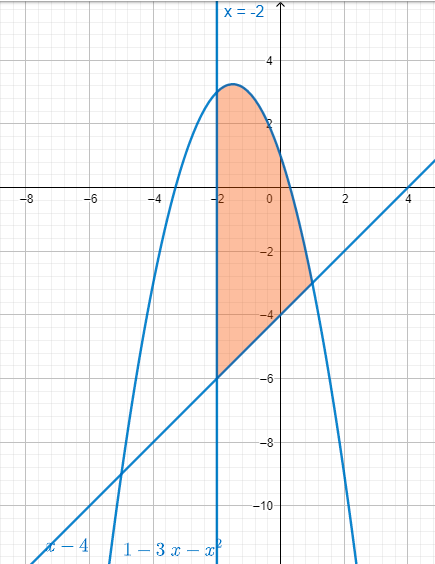
\includegraphics[scale=0.4]{img/image-20200506104639920.png}

\end{example}
\vspace*{6\baselineskip}


\begin{example}

Find the area between \(y=\sin x\cos x\) and \(y=\sin x\),
\(-\pi/2\le x\le \pi\).

\end{example}
\vspace*{6\baselineskip}

\begin{example}

Find the area between \(x=y^2-y-5\) and \(x=y+3\).

\end{example}
\vspace*{6\baselineskip}


\begin{example}

Evaluate the integral by interpreting it as the area between two curves
\[\int_0^3|\sqrt{x+5}-x|\, dx\]

\end{example}
\vspace*{6\baselineskip}


\subsection{Practice}

\begin{exercise}

Find the area between \(y=x^2+2\) and \(y=2x+5\).

\end{exercise}
\vspace*{6\baselineskip}


\begin{exercise}

Find the area enclosed by \(y=\cos\theta\), \(y=0.5\), \(x=0\), and
\(x=\pi\).

\end{exercise}
\vspace*{6\baselineskip}


\begin{exercise}

Find the area between \(y=|x|\) and \(y=x^2\).

\end{exercise}
\vspace*{6\baselineskip}

\begin{exercise}

Find the area between \(y=x\) and \(x=y^2\).

\end{exercise}
\vspace*{6\baselineskip}

\begin{exercise}

Find the area between \(x= - 3+y^2\) and \(x=y - y^2\).

\end{exercise}
\vspace*{6\baselineskip}

\begin{exercise}

Find the area between \(y=\sin x\) and \(y=\cos x\) over \([ - \pi,\pi]\).

\end{exercise}



\end{document}
